\documentclass[11pt,a4paper,twoside,openright,english,italian]{book}

\usepackage{uniudtesi}
\graphicspath{{./img/}}
\usepackage{commands}

\includeonly{./tex/glossario,./tex/titolo,./tex/abstract,./tex/intro,./tex/bitcoin,./tex/sicurezza,./tex/privacy,./tex/appendice,./tex/correlati,./tex/mining,./tex/scripting}

\newglossaryentry{blocco}{
	name=blocco,
	description={}
}

\newglossaryentry{btc}{
	name=BTC,
	description={Bitcoin intesa come unità di misura della moneta elettronica}
}

\newglossaryentry{satoshi}{
	name=satoshi,
	description={Unità di misura del valore di una transazione utilizzata all'interno della struttura dati. 1 BTC = 100000000 satoshi}
}

\makeglossaries
\makeindex

\begin{document}

\hypersetup{
  % pdfpagelayout=SinglePage, % default
  % pdfpagemode=UseOutlines, % default
  bookmarksopen, % default
  bookmarksopenlevel=2, % default;
  pdftitle={BitCoin},
  pdfauthor={Matteo Paoluzzi},
  pdfsubject={Moneta Elettronica Peer-to-Peer},
  pdfkeywords={p2p bitcoin}}

\titolo{BitCoin\\Moneta Elettronica\\Peer-to-Peer}
%\laureanda{Giovanna Tesista}
\laureando{Matteo Paoluzzi}
\annoaccademico{2012-2013}
\facolta{Scienze Matematiche, Fisiche e Naturali} % (default)
%\corsodilaurea{Informatica} % per la laurea vecchio ordinamento
\corsodilaureatriennalein{Informatica}
%\corsodilaureaspecialisticain{Informatica}
%\corsodilaureamagistralein{Matematica}
\relatore[Prof.]{Ivan Scagnetto}
%\correlatore{Talaltro dei Tali}
%\correlatoreDue{Secondo Correlatore}
\dedica{Ai miei genitori\\ per non avermi tagliato i viveri, \\ \\ a Serena\\ per il continuo e incessante supporto} % (facoltativo)


\frontmatter
\maketitle

\begin{abstract}
Verrà descritta la struttura e il funzionamento della rete Bitcoin, un sistema monetario decentralizzato virtuale.
Per prima cosa si procederà ad un raffronto tra le altre tipologie di reti P2P e la rete Bitcoin, evidenziandone le differenze e il perché tale rete sfugga ai normali criteri di catalogazione, pur rientrandone sotto alcuni punti di vista ben specifici.
Verrà poi analizzata la rete nello specifico, illustrandone scopi, funzionamento, utilizzi e criticità, queste ultime soprattutto a confronto con le altre tipologie di rete nei casi attinenti.
Infine verranno trattati in modo informale alcuni temi di carattere socio-economico collegati all'utilizzo di Bitcoin, analizzando brevemente alcune vicende di cronaca che negli ultimi anni hanno avuto tra i protagonisti tale rete.
\end{abstract}

\%\selectlanguage{english} \%\textbackslash{}begin\{abstract\}
\%Sommario della tesi in inglese \%\textbackslash{}end\{abstract\}
\%\selectlanguage{italian}

\tableofcontents
%\listoffigures
%\listoftables

\mainmatter
\chapter{Panoramica generale sulle reti P2P}\label{panoramica-generale-sulle-reti-p2p}

Negli ultimi anni si è assistito ad una progressiva alterazione delle "leggi" che regolano il mondo dell'hardware informatico in campo consumer: l'aumento della potenza di calcolo del singolo elaboratore non è più economicamente conveniente\footnote{Come anche previsto da Moore: \url{https://it.wikipedia.org/wiki/Legge_di_Moore\#Seconda_legge_di_Moore}}.

Per fortuna la soluzione è stata immediata e consiste nello sfruttamento di più elaboratori collegati in rete che condividono (genericamente parlando) risorse. Sebbene per compiti specifici risulti spesso conveniente creare una rete ad-hoc, per l'utilizzo di tutti i giorni da parte dell'utente comune, la rete per eccellenza risulta essere senza ombra di dubbio la rete Internet. A causa di questa sua centralità, è stata scelta come base per lo sviluppo di applicazioni dedicate alla condivisione di risorse di vario tipo da parte di utenti con interessi in comune, creando di fatto una sottorete virtuale fondata sulla rete Internet.
%TODO sistemare sta frase scritta da cani

Questa convidisione di risorse da parte di utenti per un interesse comune definisce il nucleo di quelle che vengono chiamate \textbf{reti Peer-to-Peer}, da qui in avanti abbreviate come \emph{reti P2P}. Data la grande diffusione di queste reti e i loro svariati obiettivi, è comprensibile che ci siano molti disaccordi sulla definizione esatta di \emph{rete P2P}.

Una classificazione molto adatta agli scopi di questo documento è quella presente in \cite{core-concepts-p2p} che distingue tre diversi livelli di rete:

\begin{enumerate}
\def\labelenumi{\arabic{enumi}.}
\item
  \textbf{Infrastrutture P2P}, il cui scopo è porre le basi per i   livelli successivi fornendo funzioni di comunicazione, integrazione e   ``traduzione'' tra le varie componenti della rete. In particolare   forniscono servizi che permettono la localizzazione e la comunicazione   tra gli utenti (da ora in avanti \textbf{peer}) e l'identificazione,   l'utilizzo e lo scambio delle risorse, oltre che l'implementazione   delle politiche di sicurezza quali autenticazione e autorizzazione.
\item
  \textbf{Applicazioni P2P}, che utilizzano i servizi offerti dal   livello di infrastruttura per offrire all'utente (qui inteso come   essere umano interagente con la macchina, la quale è il peer vero e   proprio) le funzionalità della rete. Sono in pratica le interfacce tra   l'infrastruttura e la persona.
\item
  \textbf{Fenomeni sociali} derivanti dall'utilizzo delle applicazioni   P2P. Spesso infatti la forte coesione di intenti tra gli utenti di una   rete P2P porta alla nascita di comunità virtuali, centri di   aggregazione e correnti di pensiero che esulano dalla sfera   prettamente informatica.
\end{enumerate}

Come si vedrà più avanti nel corso della trattazione, la rete Bitcoin è caratterizzata da tutti e tre i livelli in modo molto più peculiare di altre reti P2P maggiormente diffuse e famose.

\section{Distribuzione dei file in una rete P2P}\label{distribuzione-dei-file-in-una-rete-p2p}

La risorsa indubbiamente più abbondante e facilmente condivisibile è lo spazio di archiviazione, per questo le reti P2P in cui vengono condivisi file sono tra le più diffuse e variegate. La loro diffusione è talmente ampia che spesso l'intero concetto di rete P2P viene ridotto a quello di rete P2P per file-sharing, motivo per cui la classificazione delle reti P2P intese in senso generico spesso si fonda sul metodo di condivisione dei file, anche quando questo non è lo scopo della rete.

Indugiando in questa generalizzazione, studieremo un caso tipico: lo scaricamento di un file attraverso il modello classico client-server e alcune reti P2P ad ampia diffusione.

Prima di cominciare è necessario chiarire un concetto che spesso è causa di confusione: il modello P2P non è una alternativa al modello client-server, bensì una sua reimplementazione meno gravosa per il server.

Infatti, se nel modello client-server ``puro'' i ruoli sono definiti ed immutabili dall'inizio della comunicazione fino al suo completamento, quando si comunica in P2P i ruoli sono relativi al collegamento esistente tra i peer.

Prendiamo il caso in cui il peer \textbf{A} voglia ottenere dal peer \textbf{B} il file \emph{file.txt}. All'inizio della comunicazione il peer \textbf{A} sarà il client e il peer \textbf{B} sarà invece il server. Immaginiamo che, mentre questo transferimento è in atto, un terzo peer \textbf{C} voglia avere il file \emph{file.txt}.

Se ci troviamo al di fuori di una rete P2P (ad esempio nel normale download di un file da internet tramite browser), i ruoli di \textbf{A} e \textbf{B} non subiscono variazioni e il peer \textbf{C} assume il ruolo di client del server \textbf{B}, il quale dovrà ottimizzare le sue risorse di banda e cpu per servire sia \textbf{A} che \textbf{C} contemporaneamente\footnote{Da questo discorso esulano tematiche quali il multitasking della cpu: il punto di vista è quello di un ipotetico utente che osserva la macchina in tempo reale}.

All'interno di una rete P2P invece, nel momento in cui comincia a scaricare \emph{file.txt}, \textbf{C} è consapevole che \textbf{B} ne possiede una copia completa e \textbf{A} una parziale e, contemporaneamente, \textbf{A} verrà informato che \textbf{C} sta scaricando lo stesso file. Quello che succede è che \textbf{B} farà da server per \textbf{A} e \textbf{C} (i quali saranno i suoi client), mentre \textbf{A} e \textbf{C} si scambieranno le parti di \emph{file.txt} che mancano l'uno all'altro (ovvero saranno sia client che server contemporaneamente). Il risultato è una sostanziale ottimizzazione delle risorse a disposizione nella rete e una maggiore velocità di ``diffusione'' del file.

Il linguaggio sopra adottato è forzatamente generico: ciò deriva dall'ampio numero di reti P2P per il filesharing esistenti, ognuna delle quali implementa a modo suo le casistiche di aggiunta/rimozione (\emph{churn}) di un peer (chiamato solitamente \textbf{nodo} nell'ambito del file sharing) dalla rete, la ricerca dei file e il trasferimento dei contenuti, tutti comunque rispettando il procedimento generico sopra descritto.

\subsection{Scalabilità}\label{scalabilituxe0}

Analizziamo la questione da un punto di vista più formale. Avremo bisogno dei seguenti dati.

\begin{description}
\item[$u_s$]
frequenza di upload verso il server
\item[$u_i$]
frequenza di upload dell'$i-$esimo peer
\item[$d_i$]
frequenza di download dell'$i-$esimo peer
\item[$F$]
dimensione in bit del file da distribuire
\item[$N$]
numero di peer che vuole una copia del file
\item[$D_{cs}$]
tempo di distribuzione del file per l'architettura client-server
\end{description}

Per semplificare i conti senza invalidarne l'efficacia, assumiamo che la rete in esame sia priva di ``disturbi'' e sia dedicata esclusivamente allo scambio di file in esame senza altre comunicazioni passanti su di essa.

\subsubsection{Caso Client-Server}\label{caso-client-server}

Osservazioni:

\begin{itemize}
\item
  Il server deve trasmettere il file a $N$ peer, quindi $NF$ bit. Data   la frequenza di upload $u_s$, il tempo per distribuire il file deve   essere almeno $NF/u_s$.
\item
  sia $d_{min} = \min\{d_1,d_p,\cdots,d_N \}$ la frequenza di download   del peer con il valore più basso. Tale peer riceverà il file in almeno   $F/d_{min}$ secondi, che è quindi il tempo minimo di distribuzione.
\end{itemize}

Da cui

\[D_{cs} \geq \max \left\lbrace \frac{NF}{u_s}, \frac{F}{d_{min}} \right\rbrace\]

Questo è il limite inferiore al tempo di distribuzione minimo per l'architettura client-server. Trattiamo il caso ottimo e consideriamolo come il tempo di distribuzione effettivo, ovvero:

\[D_{cs} = \max \left\lbrace \frac{NF}{u_s}, \frac{F}{d_{min}} \right\rbrace\]
 Da questa ultima espressione si vede come per $N$ sufficientemente grande, il tempo di distribuzione è dato da $NF/u_s$, stabilendo quindi che esso aumenta linearmente all'aumentare del numero $N$ dei peer.

\subsubsection{Caso P2P}\label{caso-p2p}

La situazione cambia nel caso di architetture P2P, in cui ciascun peer assiste il server nella distribuzione del file. Dato che bisogna tenere conto di come ogni singolo peer distribuisce le sue porzioni di file, il calcolo risulta molto complesso. Possiamo però ottenere una semplice espressione del tempo minimo di distribuzione. A tale scopo bisogna fare alcune osservazioni:

\begin{itemize}
\item
  All'inizio dell'analisi solo il server possiede il file completo. È   quindi necessario inviare ogni singolo bit del file all'interno della   rete almeno una volta perché sia trasmesso alla comunità, quindi il   minimo tempo di distribuzione è almeno $F/u_s$. La prima differenza è   già visibile: dato che i peer ridistribuiscono i file, non è   necessario che il server invii due volte lo stesso bit.
\item
  Vediamo anche che il peer con la frequenza di download più bassa non   può ottenere il file in meno di $F/d_min$ secondi.
\item
  Infine osserviamo come la capacità di upload della rete è quella del   server più quella di ciascun peer. Denotando questo valore con   $u_{tot}$ e sapendo che il numero totale di bit da trasferire è $FN$,   possiamo stabilire che il tempo di distribuzione minimo è almeno   $FN/u_{tot}$.
\end{itemize}

Unendo le affermazioni precedenti in una unica formulazione otteniamo il tempo minimo di distribuzione per una rete P2P:

\[ D_{P2P} \geq \max \left\lbrace \frac{F}{u_s}, \frac{F}{d_{min}}, \frac{NF}{u_s + \sum_{i = 1}^N u_i} \right\rbrace \]

\subsubsection{Confronto}\label{confronto}

Per un confronto diretto tra le due architetture, poniamo $F/u = 1 \text{ora}$, $u_s = 10u$ e $d_{min} \geq u_s$, ovvero abbiamo posto che un peer può trasmettere l'intero file in un'ora, la frequenza di trasmissione del server è 10 volte quella del peer e (per semplificare) le frequenze di trasmissione dei peer sono grandi abbastanza da essere irrilevanti. Otteniamo la figura \ref{img_kurose}.

\begin{figure}[htbp]
\centering
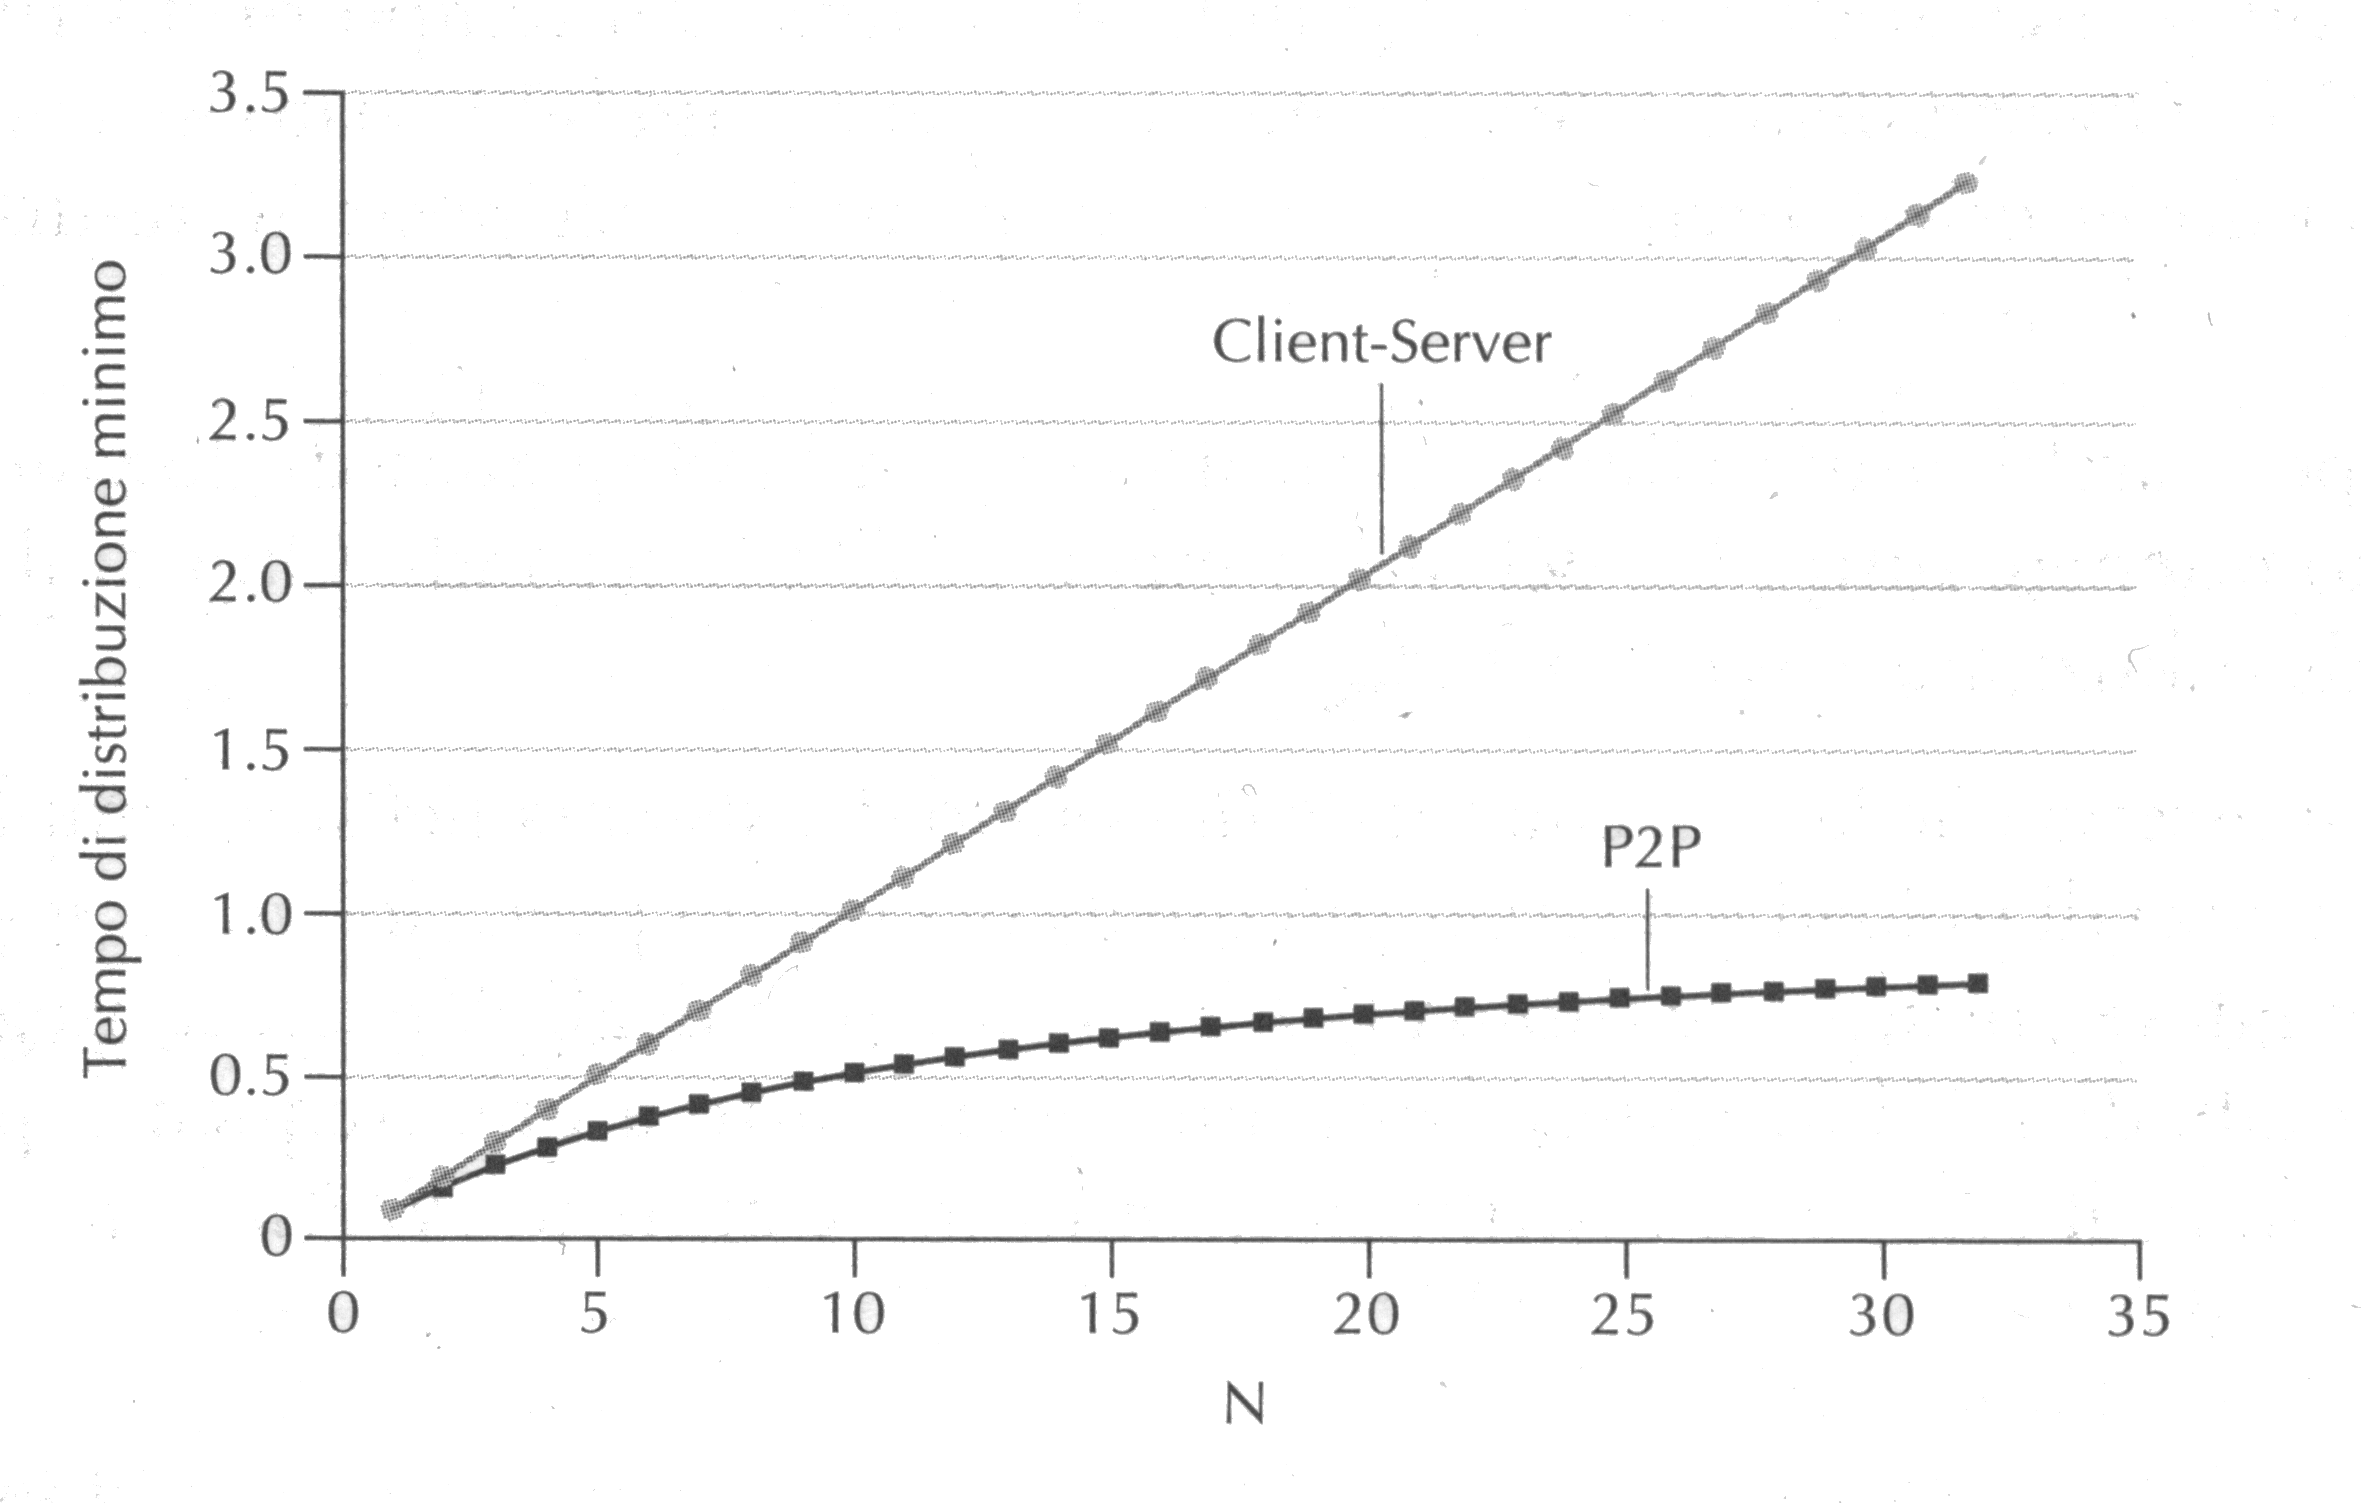
\includegraphics[scale=1]{kurose.png}
\caption[Tempi di distribuzione]{Tempi di distribuzione a confronto per le architetture P2P e client-server.\label{img_kurose}}
\end{figure}

Si nota subito che per l'architettura client-server il tempo di distribuzione risulta essere lineare come calcolato, ma ancora più notevole è il tempo di distribuzione per l'architettura P2P che non solo è sempre minore della controparte client-server, ma addirittura risulta quasi costante all'aumentare del numero dei peer. Questo dimostra come le reti P2P siano estremamente scalabili, e non c'è da stupirsi come il successo di una particolare rete dipenda essenzialmente dal numero di peer presenti. %FIXME: questa è detta molto male.

\subsection{Ricerca di informazioni}\label{ricerca-di-informazioni}

Si è parlato all'inizio della sezione di come i peer siano consapevoli di cosa altri peer stanno scaricando. Questo sottointende che esiste un sistema all'interno della rete per stabilire quanti peer sono connessi e cosa stanno condividendo e/o scaricando. Ciò significa che tale meccanismo si deve attivare ogniqualvolta un peer si (dis)connette (d)alla rete e un file viene rimosso/aggiunto. L'operazione di aggiunta/rimozione dinamica di un peer/file prende il nome di \textbf{churn}. Vediamo quindi come è possibile ricercare informazioni all'interno di una rete P2P quindi, nello specifico del file-sharing, e come sia possibile per un peer sapere quali file sono a disposizione presso quali altri peer.

\subsubsection{Directory centralizzata}\label{directory-centralizzata}

La prima, grande applicazione P2P commercializzata (\emph{Napster}) faceva uso di un indice centralizzato localizzato su un potente sever centrale. Quando un utente si collegava alla rete, l'applicazione Napster informava tale server dell'indirizzo IP della macchina e del nome dei file che l'utente aveva scelto di condividere con la rete. Il server raccoglieva quindi queste informazioni da tutti i peer collegati e aggiornava il proprio indice collegando ciascun nome di file agli indirizzi IP dei peer che in quel momento lo stavano condividendo. Ovviamente alla disconnessione di un peer l'indice veniva aggiornato di conseguenza.

Si noti come questa fosse di fatto un'architettura ibrida: client-server nella ricerca dei contenuti, P2P nel trasferimento degli stessi.

La semplicità di questo metodo nasconde però alcuni gravi difetti. Il server dell'indice si trova infatti ad essere l'anello debole della rete: un suo guasto ha come conseguenza il crollo dell'intera rete, impedendo di fatto le ricerche. Inoltre tale server deve potenzialmente gestire milioni di utenti contemporaneamete (in quanto si è visto che la potenza delle reti P2P sta nel numero di peer) e quindi risulta essere estremamente costoso da installare e mantenere, oltre a rappresentare un potenziale collo di bottiglia per l'intera rete (Napster era infatti nota per i gravi problemi di traffico da cui era afflitta).

Esiste inoltre un terzo problema non strettamente tecnico ma fondamentale per l'argomento di questo documento: \textbf{la privacy dell'utente}. Con un indice centrale che associa un file ad una serie di IP, è facile per chiunque vedere chi possiede cosa, soprattuto nel caso in cui i file condivisi rappresentino una violazione del diritto d'autore. Pur essendo il caricamento dei file una responsabilità dei singoli utenti e non di chi fornisce il servizio, molte legislazioni internazionali prevedono leggi per la tutela del copyright che possono costringere il proprietario del server ad interrompere il servizio, bloccando così l'intera rete, anche quei peer che condividevano materiale lecito. Questo controllo a volte molto invasivo (se non dannoso) da parte di terze parti non coinvolte nella rete è uno dei motivi che ha portato alla nascita di reti sempre più decentralizzate, come appunto la rete Bitcoin.

\subsubsection{Query flooding}\label{query-flooding}
 Rimanendo nell'ambito della ricerca di informazioni per file-sharing, la soluzione diametralmente opposta alla precedente risiede nell'approccio completamente distribuito del query flooding, implementato originariamente dal protocollo \textbf{Gnutella}. Questo approccio prevede che l'indice sia distribuito all'interno della comunità, in particolare ogni peer indicizza solamente quello che intende condividere con gli altri peer.

Il protocollo Gnutella prevede che ogni peer sia collegato al massimo a dieci altri nodi dell'overlay network, nodi che vengono denominati \emph{vicinato}. Se un peer vuole cercare un file, invia messaggi di ricerca ai suoi vicini, i quali instradano tali messaggi ai loro vicini che ripetono l'operazione e così via. Questo è il processo del \emph{query flooding} in cui la rete viene ``sommersa'' (\emph{flood}) di richieste (\emph{query}). Quando un peer riceve una query, controlla se nel suo indice è presente una qualche corrispondenza e, in caso affermativo, invia al peer che ha effettuato la richiesta un messaggio di successo (\emph{query-hit}) contenente il nome del file e la dimensione. La query-hit viene inviata al nodo che ha effettuato la ricerca seguendo lo stesso percorso seguito dal pacchetto query. Dopo qualche tempo il peer di origine avrà un elenco di peer che condividono file corrispondenti alla sua richiesta.

Ma anche in questo approccio, la semplicità nasconde alcune problematiche. La più grave riguarda le ricerche, che vengono propagate all'intera rete di copertura generando una enorme quantità di traffico nella rete sottostante (nel caso di Gnutella, Internet) che connette i peer. Come soluzione a tale problema si è inserito nei messaggi di ricerca di Gnutella un campo \emph{time-to-live}, il quale viene decrementato da ogni peer prima di reinoltrare la richiesta: quando il campo arriva a 0 la richiesta non viene più inoltrata, limitando quindi il raggio di azione della query. Tuttavia in questo modo si riduce anche il numero di peer contattati e la probabilità di ricevere una query-hit.

Esiste inoltre una difficoltà intrinseca alle reti P2P che Napster aveva evitato: il churn. Il protocollo Gnutella tenta di risolvere il problema in questo modo:

\begin{enumerate}
\def\labelenumi{\arabic{enumi}.}
\item
  Per prima cosa, un peer, chiamiamolo X, che vuole connettersi alla   rete deve conoscere almeno un altro peer che è già connesso alla rete   (\textbf{problema del bootstrap}). I due approcci più comuni   consistono nel mantenere in ogni peer una lista di client noti a cui   tentare di connettersi e/o, in mancanza di connessione a tali nodi,   nello scaricare una lista di nodi attualmente online da un sito
  \emph{tracker}.
\item
  Dopo aver ottenuto i nodi di bootstrap, X deve tentare di connettersi   ad ognuno di questi nodi, fino a riuscirci con uno che chiameremo Y.
\item
  Dopo la connessione, X invia ad Y un messaggio di \emph{ping}   contenente un campo contatore di peer. Y inoltra tale messaggio a   tutte i nodi nella sua rete di copertura, i quali continuano l'inoltro   fino a quando il contatore non si azzera.
\item
  Ogni volta che un peer Z riceve il \emph{ping}, risponde inviando un   messaggio \emph{pong} contenente il proprio IP attraverso la rete di   copertura fino ad X.
\item
  Grazie ai messaggi \emph{pong}, X viene a conoscenza di moltri altri   peer online (quanti dipende dal contatore impostato nel messaggio   \emph{ping}) e può tentare di connettersi ad essi per ampliare il suo   vicinato.
\end{enumerate}

\subsubsection{Copertura gerarchica}\label{copertura-gerarchica}

Avendo descritto gli approcci diametralmente opposti, vediamo ora la proverbiale via di mezzo, il modello di copertura gerarchica. L'obiettivo è ottenere il meglio dalle due implementazioni sopra descritte, e fu per la prima volta realizzato da FastTrack, un protocollo implementato in Kazaa e Morpheus. Una variante di questo modello è tutt'oggi utilizzata dall'evoluzione di Gnutella, Gnutella2. Come per il query flooding, anche questo è un modello decentralizzato, ma a differenza di esso (e a discapito del principio Peer-to-Peer) non tutti i peer sono uguali: come il nome fa suggerire, esiste una gerarchia di peer che assegna a quelli più potenti (leggasi, quelli con più banda) alcune responsabilità in più designandoli come leader per altri peer. Ogni nuovo peer deve stabilire una connessione con un leader a cui notifica tutti i file che intende condividere, creando quindi una sorta di mini indice centralizzato rispettavamente ai peer connessi a quel leader (solitamente nell'ordine del centinaio). A differenza del modello centralizzato però, i leader non sono server dedicati, bensì peer veri e propri in collegamento tra di loro. Il risultato è che i leader sono collegati ad una rete di copertura del tutto simile a quella del modello query flooding, modello utilizzato infatti per l'inoltro delle ricerche. La ricerca di un file da parte di un peer segue quindi due fasi: una richiesta al proprio leader che provvede a consultare il suo indice e una eventuale propagazione della richiesta tramite query flooding da parte del leader agli altri leader. Questa struttura ``a strati'' permette quindi la connessione di molti peer senza generare una quantità eccessiva di traffico nella rete ``ospite''.

\subsubsection{DHT (Distributed Hash Table)}\label{dht-distributed-hash-table}

Crea un indice completamente distribuito che fa corrispondere gli identificatori dei file alla loro posizione. Consente agli utenti di determinare tutte le posizioni di un file senza generare un'eccessiva quantità di traffico di ricerca. Overnet (Kademlia) sfrutta DHT come anche BitTorrent.\\
Esistono numerose implementazione di DHT, ma esulando tutte dall'ambito di questa trattazione si invita per approfondimento a consultare \cite{distributed-computing}.

%\chapter{Un'analisi più approfondita delle reti
P2P}\label{unanalisi-piuxf9-approfondita-delle-reti-p2p}

NOTA BENE: TUTTA STA ROBA NON SERVE PER BITCOIN. SI TRATTA DI UN
APPROFONDIMENTO GENERICO PER RETI DI FILE SHARING IN CUI RISULTA
FONDAMENTALE INDIVIDUARE CON PRECISIONE UN SINGOLO NODO O UN SINGOLO
FILE. TUTTO QUESTO IN BITCOIN NON ESISTE.

////

Riprendiamo ora in modo più rigoroso i concetti generali espressi in
precedenza. Chiamiamo il tipo di rete in analisi \emph{P2P overlay} e la
definiamo come un grafo virtuale che connette i peer e che viene
utilizzato per la ricerca di risorse, lo storage di file e gli algoritmi
di gestione. È bene notare che la P2P overlay si trova a livello di
applicazione, mentre le comunicazioni tra i peer sono punto-a-punto una
volta che la connessione è stata stabilita.

Una P2P overlay può essere \emph{strutturata} o \emph{destrutturata}, a
seconda della tipologia di connessione del grafo che la rappresenta. Nel
caso strutturato è facile definire algoritmi precisi per la gestione
delle risorse condivisi, mentre in grafi destrutturati l'approccio è più
``alla buona'' e richiede spesso l'utilizzo di tecniche di flooding o di
\emph{random walk} come nel casodi Gnutella.

\section{Indicizzazione dei dati e
overlays}\label{indicizzazione-dei-dati-e-overlays}

Qualsiasi sia la sua struttura, ammesso che ne abbia una, una rete P2P
sfrutta una qualche forma di indice per localizzare i dati al suo
interno. Possiamo distinguere tre metodologie diverse di indicizzazione:

Indice centralizzato: Vengono utilizzati alcuni server centrali che
mantengono la posizione dei vari dati sui vari nodi. Questo è il metodo
utilizzato nelle ricerche DNS e nelle prime reti P2P come Naptser.

Indice distribuito: L'indice generale è distribuito tra tutti i peer.
Per accedere agli indici nella overlay viene utilizzata una struttura.
Creare un indice distribuito efficente è una sfida molto complessa, e
tra tutte le soluzioni proposte negli anni quella \emph{tabella hash
distribuita} (\emph{DHT}) è tra le più efficaci. Esistono infatti molte
varianti diverse dello schema DHT, ognuna con i propri algoritmi,
vantaggi e debolezze, ma lo schema tipico prevede l'utilizzo di uno
spazio delle chiavi piatto che mappa i nodi della rete con i dati in
essi contenuti /// TODO: immagine della mappa in prof 680. Nello
specifico, l'indirizzo di un nodo viene mappato ad un identificatore
nello spazio delle chiavi tramite una apposita funzione di hash. Allo
stesso modo, ogni dato del nodo viene mappato nello stesso spazio delle
chiavi tramite hash.

Indice locale: Ogni peer mantiene un indice dei propri dati locali e di
quei dati remoti per cui deve effettuare una ricerca. È una forma di
indicizzazione spesso utilizzata in reti non strutturate in cui è
necessaria una query flood, come ad esempio Gnutella.

Esiste un altro criterio per classificare un meccanismo di
indicizzazione, basato sulla semantica. Un \emph{indice semantico} è
utilizzabile anche da un essere umano e può essere il nome di un file,
una parola-chiave, una chiave in un database. Si parla di \emph{indice
libero da semantica} quando non è leggibile da un essere umano, e spesso
corrisponde ad un indice basato su funzioni matematiche come quella di
hash, ad esempio lo schema DHT sopra descritto. Il vantaggio del primo
rispetto al secondo sta nella possibilità di effettuare ricerche tramite
parole chiavi, ricerche per range e anche ricerche basate su risultati
approssimativi \footnote{ad esempio ricercare tutte le stringhe che
  iniziano, finiscono o contengono una sottostringa o una espressione
  regolare.}, tutte cose non supportate in un indice senza semantica.

\subsection{Indici distribuiti (///TODO: probabilmente posso
eliminare)}\label{indici-distribuiti-todo-probabilmente-posso-eliminare}

In una overlay strutturata, la rete P2P ha una topologia ben definita e
i dati sono localizzati secondo un criterio deterministico dipendente da
algoritmi precisi. L'obiettivo di questa precisa struttura è fornire una
ricerca molto rapida e deterministica per le query, pertanto tali
sistemi vengono definiti \emph{sistemi di lookup} e tipicamente
sfruttano tabelle di hash per localizzare i dati. Oltre allo svantaggio
sopra indicato dell'impossibilità di effetture query approssimative, il
calcolo dell'hash per ogni risorsa condivisa dai peer genera un certo
overhead che potrebbe essere particolarmente gravoso in fase di churm.

D'altro canto, in una overlay non strutturata, dato che non esiste un
metodo per stabilire la posizione di un file o di un nodo all'interno
della rete, viene usato un \emph{indice locale} per ogni peer. Pur
facilitando il churm, una query eseguita in questa rete può generare un
grande numero di messaggi e un grande ritardo per la risposta. Tale
svantaggio viene però bilanciato dalla possibilità di effettuare query
approssimative. Nonostante l'assenza di un struttra definita, emergono
alcune topologie, a seconda della funzione statistica che lega i nodi:

\textbf{Power law random graph} (PLRG): Questa topologia viene
rappresentata da un grafo casuale in cui ogni nodo ha un certo numero di
vicini (\emph{grado}) e si relaziona con gli altri nodi in base alla
\emph{Legge della Potenza} \footnote{Si tratta di una relazione
  funzionale tra due quantità in cui una quantità varia in base ad una
  potenza dell'altra.}. Se ordiniamo i nodi in base al grado, allora
l'$i$-esimo nodo avrà $c/i^\alpha$ vicini con $c$ costante.

\textbf{Normal random graph}: In questo nodo la distribuzione dei nodi
risponde alla distribuzione normale, per cui il grado di ogni peer
risulta essere tipicamente uniforme.

\section{Overlay non strutturati}\label{overlay-non-strutturati}

Essendo privi di algoritmi per il posizionamento di dati e nodi, una
ricerca eseguita in queste reti presenta alcune sfide che vale la pena
trattare.

\subsection{Proprietà}\label{proprietuxe0}

Come accennato, lo svantaggio principale nelle overlay non strutturate
sta nella ricerca: essa può richiedere lungo tempo e può risultare
infruttuosa anche nel caso in cui la risorsa cercata esista e sia
disponibile. Esistono però alcuni vantaggi:

\begin{itemize}
\itemsep1pt\parskip0pt\parsep0pt
\item
  Supporto le query complesse basate su range, attributi e valori
  approssimati.
\item
  Un churm elevato non rappresenta un problema, la connessione e la
  disconnessione di molti nodi risulta sempre rapida e non influisce
  sulle performance.
\end{itemize}

Tali vantaggi sono validi nella maggior parte delle implementazioni di
una overlay non strutturata, come ad esempio in Gnutella, ma se vengono
soddisfatte alcune condizioni sono valide anche le seguenti proprietà:

\begin{itemize}
\itemsep1pt\parskip0pt\parsep0pt
\item
  Se esiste un certo grado di replicazione dei dati, le ricerche
  risultano efficienti
\item
  L'utenza tipa è soddisfatta con ricerche di tipo best-effort.
\item
  Se la rete non è troppo vasta, non ci sono problemi di scalabilità
  durante la ricerca.
\end{itemize}

\subsection{Ricercare in reti non
strtturate}\label{ricercare-in-reti-non-strtturate}

Prendiamo il caso della rete Gnutella come esempio generico e
analizziamo nel dettaglio le metodologie di ricerca.

Consideriamo un sistema con $n$ nodi e $m$ oggetti. Definiamo $q_i$ come
la popolarità dell'oggetto $i$, ovvero la frazione di query rispetto al
totale che richiedono l'oggetto $i$. La popolarità può essere
equivalente per tutti gli oggetti oppure seguire la topologia PLRG
precedentemente nominata. In quest'ultimo caso nell'analisi utilizzeremo
la variante della distribuzione enunciata da Zipf (///TODO: fonte per
Zipf), particolarmente indicata per descrivere la frequenza di
un'occorrenza in un insieme di occorrenze. Con queste considerazioni
abbiamo:

\[ \sum^m_{i=1} q_i = 1 \]

dove

\[ \begin{array}{ll} 
    q_i = \frac{1}{m} & \textrm{con distribuzione uniforme} \\
    q_i \propto i^{-\alpha} & \textrm{con distribuzione di Zipf}
    \end{array}
\]

Stabiliamo poi che $r_i$ sia il numero delle copie esistenti
dell'oggetto $i$, e $p_i$ sia la frazione di tutti gli oggetti che sono
una copia di $i$. Esistono tre tipologie di distribuzione che possono
descrivere la replicazione: uniforme, proporzionale e quadratica. Per
cui:

\[ \sum^m_{i=1} r_i = R \] \[ p_i = \frac{r_i}{R} \]

con

\[ \begin{array}{ll} 
    r_i = \frac{R}{m} & \textrm{con distribuzione uniforme} \\
    r_i \propto q & \textrm{con distribuzione proporzionale} \\
    r_i \propto \sqrt{q_i} & \textrm{con distribuzione quadratica}
    \end{array}
\]

Con una replicazione uniforme, tutti gli oggetti hanno lo stesso numero
di copie e dunque le performance per tutte le ricerche sono identiche.
Con una popolarità uniforme, gli schemi di replicazione proporzionale e
quadratica si riducono allo schema di replicazione uniforme.

Per misurare le perfomance vengono impiegate varie metriche, tra le più
popolari ci sono:

\begin{itemize}
\itemsep1pt\parskip0pt\parsep0pt
\item
  La probabilità di query-hit.
\item
  Ritardo o numero di inoltri di query necessari per il query-hit.
\item
  Numero di messaggi processati da ogni nodo coinvolto nella ricerca.
\item
  Copertura dei nodi, ovvero il numero di nodi distinti visitati.
\item
  \emph{duplicazione dei messaggi}, calcolabile come
  $\frac{(\textrm{#messaggi} - \textr{#nodi_visitati})}{\textrm{#messaggi}}$.
\item
  massimo numero di messaggi in un nodo.
\item
  \emph{recall}, definitio come il numero di oggetti trovati che
  soddisfano i criteri ricercati (questa metrica è rese possibile dalle
  query complesse permesse in una overlay non strutturata).
\item
  \emph{efficienza dei messaggi}, ovvero i recall ottenuti per ogni
  messaggio.
\end{itemize}

Queste metriche potrebbero essere influenzate nel caso in cui le
ricerche non siano indipendenti l'una dall'altra. Nelle ricerche
definite \emph{guidate} infatti, un nodo mantiene alcune informazioni
ottenute dalle ricerche precedenti, in modo da ottimizzare i risultati
delle ricerche successive. Dato che esistono numerosi metodi per
raccogliere e utilizzare i dati di una ricerca, in questa trattazione si
discuteranno solo ricerche non guidate. \textbackslash{}\textbackslash{}
Abbiamo visto nel capitolo precedente il metodo di ricerca detto
\emph{flooding}, ne abbiamo visto le problematiche e analizzato la
soluzione del Time-To-Live dei pacchetti di ricerca con i suoi vantaggi
e le sue criticità. Il TTL rappresenta una sorta di miglioramento
rispetto alla prima soluzione proposta per il flooding, il
\emph{checking}. In questo metodo ogni nodo contatta il nodo di origine
della query per vedere se inoltrare o meno la query. La soluzione viene
considerata non pratica a causa dell'elevatissimo numero di messaggi
scambiati e il carico eccessivo imposto sul nodo che effettua la query,
che deve infatti gestire i messaggi di moltissimi nodi. Invece un
raffinamento ulteriore del TTL consiste nell'implementazione di un
\emph{anello di espansione}. Seconda questa strategia il nodo effettua
un primo flooding con un piccolo TTL. In caso di insuccesso, la ricerca
viene rifatta con un TTL maggiore e ripetuto all'occorrenza. Il successo
di questa strategia è tanto maggiore quanto maggiore è il numero di
repliche. In linea di massima, l'anello di espansione ha molto più
successo rispetto al TTL qualsiasi strategia di replicazione si utilizzi
e per qualsiasi tipo di popolarità, il tutto al prezzo di un leggero
aumento del ritardo. Ciononostante, tutte queste strategia sono basate
sul flooding e generano quindi messaggi duplicati.
\textbackslash{}\textbackslash{} Un'alternativa al flooding utilizzabili
in reti destrutturate è il \emph{random walk}. Come dice il nome, una
query viene inoltrata in modo casuale ad un altro nodo quando viene
ricevuta. Il random walk risolve il problema dei messaggi duplicati a
scapito di un aumento della latenza di ricerca. Per risolvere anche
questo problema si può aumentare il numero di nodi casuali a cui la
query viene inoltrata ad un valore $k$, implementando il \emph{k random
walk}. Per terminare la ricerca, la strategia più efficace consiste
nell'unire il checking con il TTL: ogni \emph{walker}, alla scadenza del
TTL, controlla con il nodo di origine della query se terminare la
ricerca o meno. Il TTL viene utilizzato per evitare la creazione di
cicli, e solitamente viene impostato ad un valore molto elevato.

Il random walk risulta più performante rispetto al flooding e offre
anche molta più scalabilità.

//// TODO: strategie di replicazione??

\section{Chord Distributed Hash
Table}\label{chord-distributed-hash-table}

Questo algoritmo per le DHT utilizza uno spazio delle chiavi piatto per
associare le mappe tra i nodi e i dati condivisi. Sia l'indirizzo del
nodo che i dati sono mappati ad un identificatore nello spazio delle
chiavi tramite una funzione di hash. Sia il mapping delle chiavi che il
mapping dei nodi dovrebbero assicurarsi che le chiavi siano
uniformemente distribuiti tra tutti i nodi. Questo inoltre riduce la
possibilità che i calcoli da effettuare durante il churm generino troppo
overhead. Nello specifico, quando un nodo lascia o si unisce ad una rete
con $n$ nodi, solamente $O(1/n)$ chiavi devono essere spostate in altri
nodi. L'algoritmo Chord supporta una sola operazione, \emph{lookup(x)},
che mappa una data chiave $x$ ad un nodo della rete. Chord salva un dato
nel nodo mappato dalla chiave di tale dato, il richiede due step:

\begin{enumerate}
\def\labelenumi{\arabic{enumi}.}
\itemsep1pt\parskip0pt\parsep0pt
\item
  Mappare il dato alla sua chiave nello spazio degli indirizzi comune.
\item
  Mappare la chiave al nodo utilizzando \emph{lookup}. La progettazione
  di \emph{lookup} è la sfida di questo algoritmo.
\end{enumerate}

In questo algoritmo, l'indirizzo IP viene passato ad una funzione di
hash che genera un identificatore di $m$ bit che identifica il nodo
nello spazio comune delle chiavi. Anche i dati vengono passati ad una
funzione di hash che genera sempre una chiave da $m$-bit. Il valore $m$
viene deciso a priori per evitare di generare collisioni con in fase di
hashing. Chord utilizza un anello logico di dimensione $2^m$, per cui lo
spazio delle chiavi è ordinato su tale anello logico con modulo $2^m$
\footnote{Nei successivi conti il modulo $2^m$ verrà sottinteso.}.

Una chiave $k$ viene assegnata al primo nodo tale che l'identificatore
di tale nodo equivale o è successivo all'identificatore della chiave $k$
nello spazio degli identificatori, e tale nodo viene chiamato
\emph{successore di k} e denotato come \emph{succ(k)}. Ad esempio, in un
anello con $m=7$ abbiamo i nodi N5, N18, N23, N28, N63, N73, N99, N104,
N115 e N119. Sei chiavi K8, K15, K28, K53, K87 e K121 vengono
distribuite tra questi nodi come segue: \emph{succ}(8)=18,
\emph{succ}(15)=18, \emph{succ}(28)=28, \emph{succ}(53)=63,
\emph{succ}(87)=99, \emph{succ}(121)=5.

\subsection{Esempi di ricerca mediante
chiavi}\label{esempi-di-ricerca-mediante-chiavi}

In un primo, semplice, algoritmo per il lookup, ogni nodo contiene solo
un valore nella sua tabella di routing e memorizza unicamente il suo
successore nell'anello dei nodi. Ogni query per la chiave $x$ viene
inoltrata tra i nodi fin quando raggiunge un nodo il cui identificatore
$y$ è maggiore della chiave $x$ modulo $2^m$. Il risultato torna al nodo
di partenza seguendo il percorso inverso. Questo semplice algoritmo
richiede $O(1)$ di spazio locale ma $O(n)$ salti tra gli $n$ nodi.

/// TODO: algoritmo 18.1 pag 690 (specificare notazione descritta in
fondo a pag 689) /// TODO: grafico di ricerca 18.2 pag 689

Una versione più raffinata del precedente algoritmo richiede l'aumento
dello spazio locale di archiviazione per le tabelle di routing a $O(n)$
ma permette di ridurre il numero dei salti tra i nodi a $O(\log n)$.
Ogni nodo $i$ mantiene una tabella di rounting chiamata di indice
(\emph{finger table}), con al massimo $O(\log n)$ valori distinti,
costruita in modo tale che l'$x$-esimo valore (con $1 \leq x \leq m$)
sia l'identificatore per il nodo \emph{succ}$(i + 2^{x-1})$ (più
formalmente \emph{i.finger{[}$x${]} = succ}$(i + 2^{x-1})$). Tale nodo
risulta essere il primo nodo la cui chiave è maggiore della chiave del
nodo $i$ per un valore pari ad almeno $2^{x-1}\text{*mod*}2^m$.

A causa della sua struttura logaritmica, la finger table contiene più
informazioni sui nodi successivi vicini rispetto ai nodi successivi
lontani \footnote{qui ``successivi'', ``vicini'' e ``lontani'' fanno
  riferimento all'anello che si viene a creare nella Chord overlay.}.
Immaginiamo infatti di cercare la chiave $k$ partendo dal nodo $i$. Se
$k$ si trova tra $i$ e il suo successore, allora vuol dire che $k$ si
trova effettivamente nel successore. Altrimenti $k$ si trova oltre il
successore, per cui $i$ deve scandire la sua finger table per
identificare il nodo $j$ che precede immediatamente $k$. Dato che $j$ si
trova più vicino a $k$ di $i$, esso conterrà molte più informazioni
utili alla localizzazione di $k$.

///TODO: gestione del churm in una Chord (pagg 691-695)

\chapter{Bitcoin: moneta elettronica decentralizzata}\label{bitcoin-moneta-elettronica-decentralizzata}

Tutte le reti P2P finora descritte sono in circolazione da molti anni, hanno una base di utenti che conta milioni di peer divisi tra utenti reali e server automatizzati, contano migliaia di forum di supporto e scambiano quotidianamente una immensa fetta del traffico totale della rete Internet (tanto che molti provider tendono a limitarne quanto più possibile l'utilizzo, soprattutto nelle fasce orarie di maggior traffico). Sono però tutte reti dedicate al file-sharing. Bitcoin no. O almeno, non proprio, come vedremo.

Bitcoin è una rete P2P (intesa per tutti e tre i livelli descritti in precedenza) che mira a creare un sistema di valuta digitale privo di controllo centrale, con pagamenti effettuati direttamente tra gli utenti senza l'intervento di terzi. È stata ideata e realizzata in origine da un anonimo noto con il nome di \textbf{Satoshi Nakamoto} \cite{bitcoin}, formalizzata con un whitepaper nel 2008 ed entrata in vigore il 3 Gennaio 2009 e si è in poco tempo evoluta in modo esponenziale fino a catturare di recente l'attenzione dei media internazionali, delle banche mondiali e, per alcuni suoi utilizzi illeciti, da FBI ed NSA. Ma vediamo di cosa si tratta.

\section{Moneta Elettronica}\label{moneta-elettronica}

\textbf{Bitcoin} è il nome dato alla rete, al client originale, al protocollo di comunicazione e alla moneta utilizzata per le transazioni all'interno della rete.

Le monete (d'ora in avanti \textbf{btc}) posso essere ottenute ``gratuitamente'' dopo aver impegnato la propria CPU o GPU in alcuni calcoli di crittografia (operazione chiamata \textbf{mining} e discussa più avanti), oppure acquistate da altri utenti della rete tramite una valuta reale \footnote{Ad esempio tramite il sito Internet Mt. Gox   \cite{mtgox}.}.

Entrambi questi metodi sono fondamentali nell'ecosistema Bitcoin:

\begin{itemize}
\item
  Il mining è una diretta conseguenza della partecipazione di un nodo   alla rete (vedi più avanti NETWORK) ed è l'unico metodo con cui   vengono create e messe in circolazioni nuove \textbf{btc}. Per ogni   operazione di mining avvenuta con successo si riceve una quantità   fissa di btc che viene dimezzata nel tempo, limitando il numero   massimo di bitcoin in circolazione a circa 21 milioni. A Gennaio 2013   è stata generata circa la metà delle monete totali e si stima di   arrivare a 3/4 nel 2017. La quota massima di moneta circolante e   l'assenza di istituti centrali in grado di creare nuove monete rendono   l'economia bitcoin invulnerabile all'inflazione che colpisce le   economie reali. Il sistema è ispirato a quella che era l'economia del   Dollaro prima della istituzionalizzazione della Federal Reserve come   banca federale: il valore del Dollaro era legato al valore corrente   dell'oro, il quale esiste in quantità limitata ed è ottenibile solo   attraverso il lavoro dei minatori.
\item
  La compravendita di bitcoin è invece simile alle compravendite di   azioni effettuate nelle borse di tutte il mondo. Esistono infatti   alcuni luoghi dedicati (ad esempio il sito internet \emph{Mt. GOX})   che fungono da stock exchange offrendo agli utenti la possibilità di   mettere in vendita o di acquistare bitcoin al prezzo che preferiscono.   Sono delle vere e proprie borse che trattano unicamente bitcoin invece   che molti titoli di aziende diverse, calcolano un valore di scambio   medio basato sulle ultime transazioni portate a termine ma lasciano   libero l'utente di scegliere a quanto vendere o comprare bitcoin, con   prezzo medio che si adegua di conseguenza. 
%FIXME sistemare sta roba   
%TODO verificare se rapporto bitcoin/euro e bitcoin/dollaro sono   legati alle transazioni in quella valuta (come credo che sia)
\end{itemize}

Come per le monete in valuta reale e le azioni borsistiche, anche le bitcoin vengono ``tenute'' in portafogli. Come vedremo, il termine \emph{tenute} è usato impropriamente, ma questa è l'apparenza dal punto di vista dell'utente, per cui a tale apparenza al momento ci atterremo.

\section{Portafogli e indirizzi}\label{portafogli-e-indirizzi}

La prima volta che un nuovo utente avvia il suo client Bitcoin fresco di installazione, si vede assegnato un portafoglio contenente un indirizzo e una copia di chiavi di cifratura simmetrica. L'indirizzo è semplicemente una stringa di 27-34 caratteri alfanumerici che inizia con un 1 o con un 3, generata in modo casuale dalle chiavi create per l'utente. Gli indirizzi rappresentano il punto di uscita e/o il punto di ingresso per tutti i movimenti che coinvolgono bitcoin. Questo significa che nelle transazioni bitcoin compariranno unicamente questi indirizzi, rendendo di fatto \textbf{anonimi} tutti i movimenti di bitcoin (meno quelli che riguardano l'acquisto di bitcoin tramite moneta reale), in un modo del tutto equivalente a quello dei conti in Svizzera. Non esiste quindi nessuna correlazione diretta e ovvia tra un utente e il suo indirizzo. Un portafogli può contenere più indirizzi: basta infatti generare una nuova coppia di chiavi e verrà generato anche un nuovo indirizzo. Il numero di indirizzi esistenti è virtualmente infinito.

I portafogli sono solitamente legati al software che li crea, basta quindi cambiare software per poter creare un nuovo portafogli e una nuova coppia di chiavi (oppure installare un software in grado di gestire più portafogli). In alternativa è possibile ``aprire un conto'' presso numeri siti che offrono questa funzionalità, quale ad esempio blockchain.info. In questo caso però bisogna fare i conti con la sicurezza del sito in questione 
%TODO link alla sezione sicurezza

\section{Transazioni}\label{transazioni}

Le transazioni rappresentano il nucleo fondamentale di bitcoin. Esse sono il metodo con cui, a livello astratto, le bitcoin vengono trasferite da un account all'altro e tramite la loro analisi ci si assicura che un indirizzo contenga esattamente quel numero di bitcoin, che una bitcoin non venga spesa più volte e che quella bitcoin appartiene a quello specifico indirizzo. Le transazioni si basano su meccanismi di crittografia a chiave pubblica, rendendo quindi obsoleto il coinvolgimento di terze parti nella transazione. Se infatti nelle normali compravendite online, volenti o nolenti si è costretti a fidarsi di terze parti che garantiscono per il buon esito dell'operazione (istituti di credito, compagnie di carte di credito, siti come Paypal, ecc), qui gli utenti hanno direttamente la prova crittografica senza aver quindi necessita di fidarsi di qualcuno.

Satoshi Nakamoto descrive la sua moneta elettronica come una serie di firme digitali. Il trasferimento di moneta da un utente all'altro avviene infatti applicando la firma digitale dell'acquirente ad un hash di una precedente transazione e della chiave pubblica del venditore, e aggiungendo ciò alla fine della moneta.

Riassumendo schematicamente:

\begin{verbatim}
hash = hash(previous_transaction, vendor_public_key)
transaction = sign(hash, private_key)
\end{verbatim}

La moneta diventa quindi non una unità atomica, ma il risultato di una serie di transazioni che coinvolgono firme digitali e verifiche che deve essere calcolato dinamicamente. La serie di tutte le transazioni mai effettuate viene raccolta in una sequenza denominata \textbf{blockchain}.

\begin{figure}[htbp]
\centering
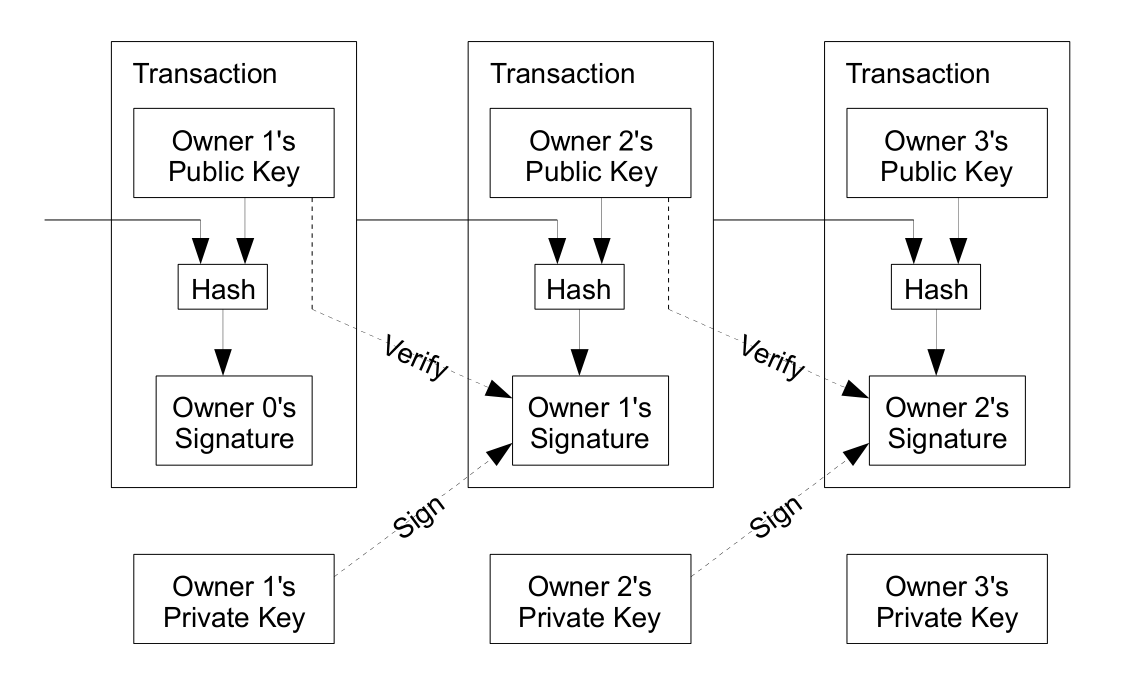
\includegraphics{bitcoin_p2_1.PNG}
\caption{Utilizzo delle chiavi e degli hash in una sequenza di transazioni.\label{bitcoin_p2_1}}
\end{figure}

Questa implementazione però non garantisce che l'acquirente non abbia già effettuato una transazione con questa moneta, ovvero che stia spendendo una moneta già spesa in precedenza.

L'unico modo per garantire ciò senza utilizzare una terza parte di cui fidarsi, è tenere conto di \textbf{tutte} le transazioni. Questo vuol dire che tutte le transazioni devono essere annunciate ad un pubblico in grado di mettersi d'accordo sull'effettivo ordine temporale in cui sono state effettuate. Il venditore deve avere quindi la prova che, nel momento in cui riceve la transazione, la maggioranza dei nodi è d'accordo che quella è la prima transazione ricevuta.i

\section{Timestamp e Proof-of-Work}\label{timestamp-e-proof-of-work}

La soluzione consiste nell'utilizzo di un \textbf{timestamp server}. Un timestamp server funziona calcolando l'hash di un blocco di oggetti di cui si vuole realizzare il timestamp e rendendo tale hash pubblico. Il timestamp dimostra inequivocabilmente che gli oggetti esistevano al momento dell'hashing. Ogni timestamp include anche il precedente timestamp nell'hash, formando quindi una catena in cui ogni timestamp rinforza \footnote{leggasi: rende più difficili da modificare.} quelli precedenti.

Ora il problema consiste nell'implementare questo server di timestamp in modo distribuito, come è appunto la rete Bitcoin. Per prima cosa bisogna trovare un sistema per cui effettuare il timestamp è un'operazione difficoltosa (computazionalmente parlando), ma verificare che il timestamp sia corretto deve essere immediato. Basandosi sul lavoro di Adam Back (\cite{hashcash}), Nakamoto ha deciso che la difficoltà dell'operazione deve essere trovare un valore che, una volta sottoposto ad hashing (ad esempio con SHA-256), il risultato sia un hash che comincia con uno specifico numero di bit pari a zero: la difficoltà del lavoro è esponenziale al numero di bit zero richiesti, ma è facilmente verificabile con un singolo hash. L'implementazione per bitcoin consiste quindi nella creazione di un blocco di dati di cui calcolare l'hash che contiene le transazioni interessate, l'hash precedente e un valore chiamato \textbf{nonce} da incrementare fino a quando l'hash non avrà le caratteristiche richieste. Modificare una transazione comporta modificare un blocco, e quindi ripetere tutto il lavoro di calcolo della nonce. Inoltre, se a questo blocco è già stato incatenato uno più blocchi successivi, anche tali blocchi andranno ricalcolati in sequenza, rendendo il lavoro estremamente gravoso.

\begin{figure}[htbp]
\centering
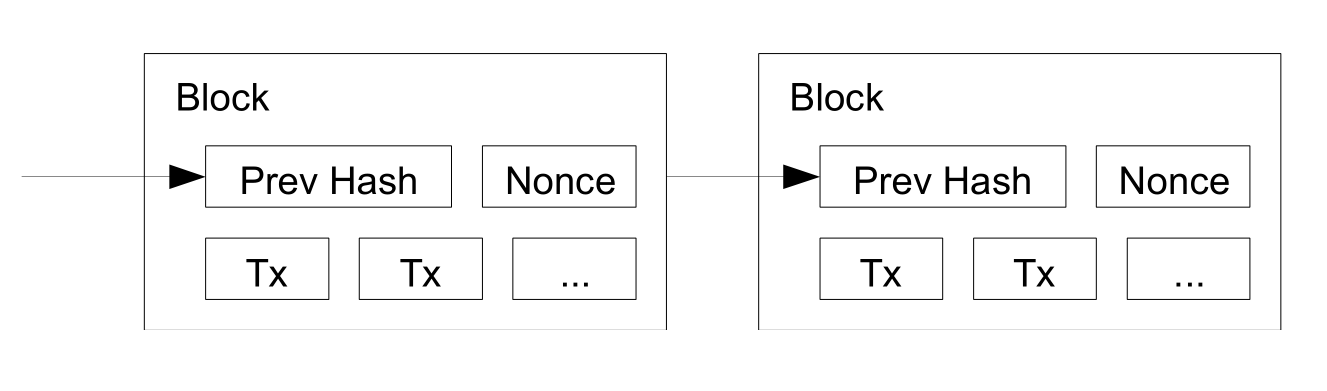
\includegraphics{bitcoin_p3_1.PNG}
\caption{Struttura minimale di una sequenza di blocchi.\label{bitcoin_p3_1}}
\end{figure}

Con la prova di lavoro si risolve anche il problema di cosa significa che la maggioranza deve accettare un timestamp. Con l'hash infatti si realizza una sorta di sistema one-CPU-one-vote, e la ``decisione della maggioranza'' è rappresentata dalla più lunga sequenza di timestamp, che è la sequenza per la quale è stata impiegata la maggior parte di lavoro computazionale. Ciò significa che se la maggior parte della forza-CPU è controllata da peer onesti (cioè che non hanno nessuna intenzione di modificare una transazione effettuata), un nodo disonesto che volesse modificare una transazione non solo dovrebbe rifare tutti i calcoli per il blocco della transazione e per tutti i blocchi successivi, ma avendo minor potenza di CPU a disposizione rispetto ai nodi onesti, verrebbe rapidamente soverchiato dal numero di calcoli da fare, in quando il numero di blocchi da ricalcolare sarebbe sempre superiori a quelli da lui già ricalcolati.

Si capisce subito che è nella rete bitcoin (e nelle reti P2P in generale) è importante che le risorse (potenza di calcolo in questo caso) siano equamente distribuite tra i peer, in modo da evitare che un solo nodo o un solo gruppo di nodi controlli l'intera rete.

Per far fronte alle differenti configurazioni hardware degli utenti, alla sempre crescente capacità di calcolo di CPU e GPU e anche ai potenzialmente mutevoli interessi dei nodi, la difficoltà della prova di lavoro (ovvero il numero di bit zero) è determinata da una media calcolata sul numero medio di blocchi generati ogni ora. Se vengono generati troppi blocchi, vuol dire che la difficoltà è troppo bassa e viene subito aumentata.

\section{Network}\label{network}

A questo punto abbiamo una prima approssimazione di come funziona la rete bitcoin:

\begin{enumerate}
\def\labelenumi{\arabic{enumi}.}
\itemsep1pt\parskip0pt\parsep0pt
\item
  Le nuove transazioni sono inviate a tutti i nodi.
\item
  Ogni nodo raccoglie le transazioni che riceve in un blocco.
\item
  Per ogni blocco, ogni nodo cerca di calcolare una proof-of-work.
\item
  Una volta trovata la prova, invia il blocco a tutti i nodi.
\item
  I nodi accettano il nuovo blocco se e solo se tutte le transazioni in   esso sono valide (si verifica calcolando l'hash delle transazioni e   confrontandole con l'ultimo blocco accettato) e non già spese in   precedenza.
\item
  Il nodo esprime la sua accettazione del blocco appena arrivato   mettendosi al lavoro per crearne uno nuovo, usando l'hash del nodo   accettato.
\end{enumerate}

I nodi considerano la catena più lunga quella corretta (e viene definita \emph{blockchain}) e lavoreranno sempre in modo da prolungarla. Esiste la possibilità che uno stesso nodo riceva due versioni diverse dello stesso blocco in contemporanea. In questo caso, lavoreranno sul prima blocco ricevuto, ma manterrano una copia anche dell'altro nel caso in cui si rivelasse appartenente alla catena più lunga. La verifica viene fatta non appena viene trovata la nuova proof-of-work e una delle due catene si allunga: a questo punto si individua il blocco da mantenere in base all'hash contenuto nel blocco appena arrivato, gli altri blocchi vengono scartati e si continua il procedimento. Inserendo un po' di terminologia, chiamiamo il primo blocco mai realizzato (che è codificato all'interno di ogni client Bitcoin) \emph{blocco genesi}, l'ultimo blocco della catena \emph{blocco di testa}, la distanza tra un blocco \emph{b} e il blocco genesi viene definita \emph{altezza}.

Quando si inviano in broadcast le nuove transazioni, non è necessario che esse raggiungano tutti i nodi: fintanto che raggiungono quanti più nodi possibile, verranno velocemente inglobate in un blocco. I blocchi invece devono essere ricevuti da tutti i nodi, per questo se un nodo riceve un blocco e si accorge (tramite hash) che il blocco precedente gli manca, ne richiederà immediatamente una copia ad un altro nodo, e ripeterà la verifica fino ad ottenere la catena integrale.

Per convenzione, la prima transazione di un blocco è una transazione speciale che crea una nuova moneta e la assegna al creatore del blocco. In pratica il primo nodo che riesce a trovare la proof-work di un nuovo blocco riceve un premio in bitcoin. Tale premio serve ad incentivare i nodi a mantenere attiva la rete ed inoltre permette la messa in circolazione di nuove monete, senza che sia necessaria una zecca centrale. Questo profitto derivante dal calcolo della proof-of-work viene denominato \textbf{mining} e ha spinto molti utenti ad acquistare hardware dedicato sempre più performante in modo da creare per primi il nuovo blocco e ottenere il relativo premio, inizialmente ammontante a 50btc ma ora dimezzato a 25btc). 
%TODO collegamento al mining

Visto che il numero massimo di btc è stato determinato a priori ed è invariabile, per incentivare i nodi anche quando il mining risulterà inutile, sono state introdotte delle vere e proprie tasse di transazione, le \textbf{transaction fees}. Una transaction fee non ha un valore fisso, ma viene decisa da chi effettua la transazione e può anche essere nulla: viene registrata come una differenza tra il valore di input e il valore di output della transazione, con quest'ultimo valore inferiore del primo (come in una tassa, l'acquirente spende più dell'importo effettivo). Tale differenza verrà trasferita nella transazione dedicata all'incentivo al momento della creazione del nuovo blocco, sempre ammesso che l'utente che ha creato il blocco voglia riceve queste btc.

Oltre ad invogliare un nodo a rimanere attivo, gli incentivi incoraggiano i nodi a rimanere onesti: infatti se un attaccante avido riuscisse ad accumulare abbastanza potenza di calcolo da surclassare quella di tutti gli altri nodi, potrebbe scegliere se truffare gli altri nodi ritirando i suoi pagamenti precedenti oppure usarla per accumulare nuove monete con gli incentivi. Un attaccante si vede quindi incoraggiato a mettere la sua potenza di calcolo a favore del sistema facendogli guadagnare più btc di tutti gli altri nodi messi insieme, invece di usare la stessa potenza per minare le basi dello stesso sistema in cui egli stessi investe i propri soldi.

\section{Risorse necessarie}\label{risorse-necessarie}

Il sito Blockchain.info \cite{blockchain-info} offre vari servizi agli utenti bitcoin, tra i quali spiccano un portafogli online, un sistema di navigazione dell'intera catena dei blocchi e dettagliate statistiche sull'intera rete. Da tale sito si vede come in media, in 24 ore vengono effettuate 56700 transazioni archiviate in 220 blocchi, il che vuol dire un blocco ogni 6.55 minuti. Se ogni nodo dovesse mantenere ogni singola transazione, lo spazio di memoria occupato renderebbe la rete bitcoin non così appetibile per l'utente medio. Risulta necessario minimizzare la quantità di memoria necessaria a mantenere la blockchain senza compromettere la sicurezza.

Si è detto infatti che l'hash di un blocco viene calcolato a partire dall'hash del blocco precedente, da una nonce e dalle transazioni contenute nel blocco. Ma invece che memorizzare le intere transazioni, esse vengono inserite come foglie di un albero di Merkle \cite{merkle}, una struttura dati in cui ogni nodo non foglia è l'hash di tutti i suoi figli, in modo che nella radice di tale albero ci sia un solo hash che riassume in se tutte le transazioni. È pertanto possibile calcolare l'hash di un blocco basandosi unicamente sull'hash del blocco precedente, sulla nonce e sulla radice dell'albero di Merkle, ovvero sull'hash riassuntivo delle transazioni, rendendo quindi possibile eliminare alcune transazioni dalla blockchain per risparmiare un poco di spazio.

\begin{figure}[htbp]
\centering
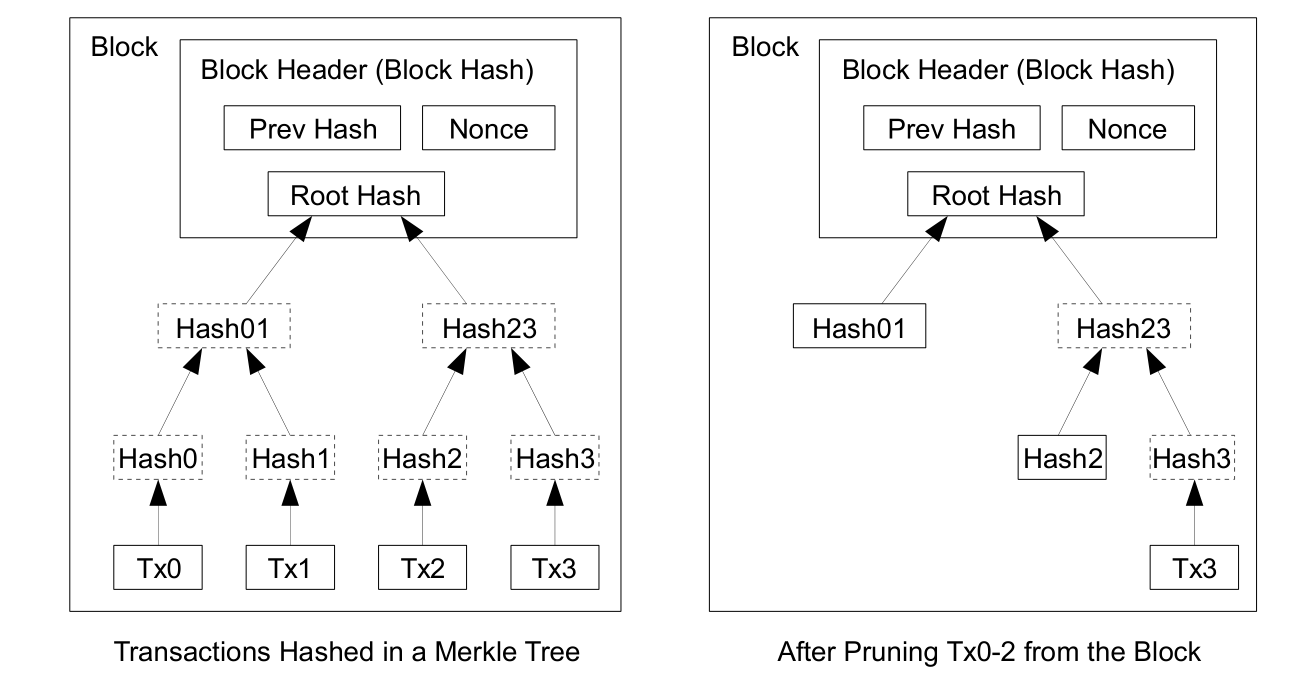
\includegraphics{bitcoin_p4_1.PNG}
\caption{Struttura di un blocco prima e dopo la compressione dell'albero delle transazioni.\label{bitcoin_p4_1}}
\end{figure}

%TODO sezione tecnica
Con questa struttura, il \textbf{block header} viene ad occupare esattamente 80 Bytes (vedi sezione tecnica per i dettagli), il che significa circa 6.2 MB all'anno (Satoshi Nakamoto con una stima di un blocco ogni 10 minuti aveva previsto 4.2 MB annui). Una quantità decisamente ridotta che rende la blockchain tollerabile su ogni computer degli ultimi 7 anni.

È possibile quindi verificare i pagamenti senza disporre di un nodo personale. L'utente deve possedere una copia degli header della catena più lunga (che può ottenere dai nodi della rete) e ottenere il ramo di Merkle che collega la transazione al blocco in cui è stata inserita. Non può verificare la transazione da solo calcolando gli hash (non ha le altre foglie dell'albero di Merkle), ma collegandola ad un punto specifico della catena può vedere che un nodo l'ha accettata, ed eventuali blocchi successivi confermano che anche l'intera rete l'ha accettata.

\begin{figure}[htbp]
\centering
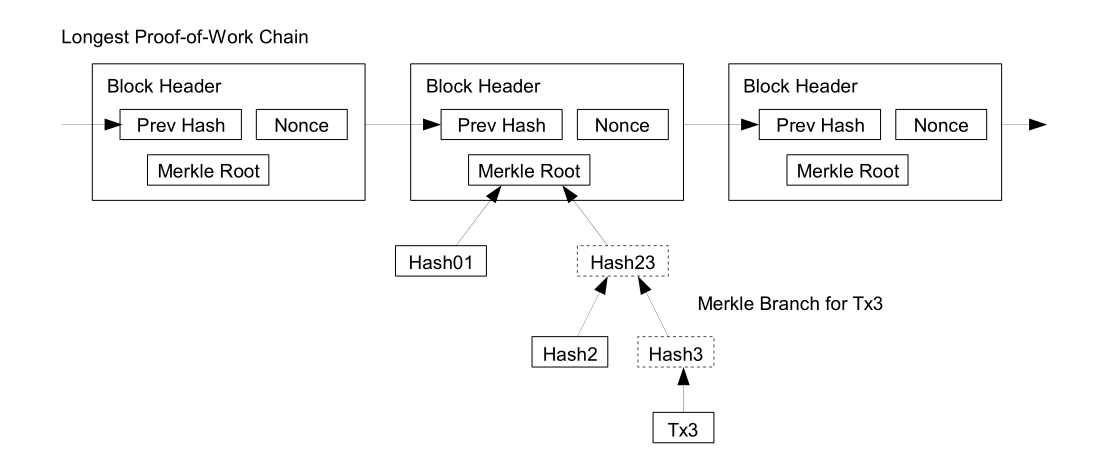
\includegraphics{bitcoin_p5_1.PNG}
\caption{Struttura di un blocco prima e dopo la compressione dell'albero delle transazioni.\label{bitcoin_p5_1}}
\end{figure}

Così come è descritta, la verifica è affidabile fin tanto che la rete è controllata da nodi onesti, ma è vulnerabile se la rete è soverchiata da un attaccante. Mentre un nodo può effettuare le verifiche da se, il metodo semplificato è vulnerabile alle transazioni ad-hoc create da un attaccante che controlla la rete. Una strategia di difesa consiste nell'accettare avvisi dai nodi della rete quando questi rilevano blocchi non validi, richiedendo all'utente di scaricare l'intero blocco. Per questo motivo chi utilizza bitcoin per business ritiene preferibile avere un nodo personale con intera blockchain, in modo da poter effettuare verifiche autonomamente e velocemente. 
%FIXME questo paragrafo è scritto male

Da questo si può dedurre un fatto importante che distingue la rete bitcoin dalle altre reti P2P: si può partecipare alla rete anche senza il relativo software (in questo senso, si partecipa al livello comunitario della rete): non serve essere un nodo, basta essere un utente.

\section{Gestione dei valori}\label{gestione-dei-valori}

Anche se è possibile trattare le monete una ad una, è improponibile fare una transazione per ogni singolo centesimo. Per la divisione degli importi, le transazioni contengono molteplici input e output. In una transazione normale si avranno o un singolo input proveniente da una grande transazione precedente oppure più input provenienti da più transazioni piccole precedenti, e al massimo due output: uno per il pagamento vero e proprio e uno per restituire il resto, se presente, al mittente.

Chiarimo meglio il concetto:

\begin{itemize}
\itemsep1pt\parskip0pt\parsep0pt
\item
  Un input è un riferimento ad un output di una precedente transazione   che contiene l'indirizzo di chi sta effettuando la transazione. Se ci   sono più input, l'importo degli output da loro referenziati viene   sommato ed il totale è il massimo valore utilizzabile dall'output.
\item
  Un output contiene l'indirizzo del destinatario e il valore da   spedire. Dato che, in una futura transazione, un output può essere   referenziato da un solo input, potrebbe verificarsi il caso in cui   l'input sia maggiore dell'output e della transaction fee desiderata.   In questo caso è necessario creare due output, uno con il valore da   spedire e l'indirizzo del destinatario, l'altro con la differenza da   restituire al mittente, il \textbf{resto}. La differenza tra il totale   degli input e il totale degli output è la transaction fee.
\end{itemize}

La situazione è visibile in \ref{bitcoinpropagation_1}.

\begin{figure}[htbp]
\centering
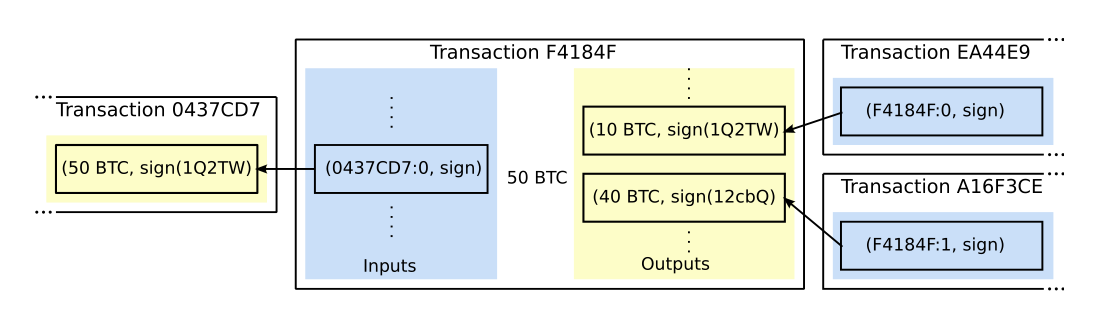
\includegraphics{bitcoinpropagation_1.PNG}
\caption{Schema di una transazione in cui vengono evidenziati input e output.\label{bitcoinpropagation_1}}
\end{figure}

Nonostante la stretta dipendenza tra le varie transazioni, non è necessario estrarre l'intero background di ogni input, in quanto la transazione verrà accettata solo se il blocco che contiene le transazioni con gli output referenziati dagli input è stato accettato dalla rete.

Dato il valore elevato di una singola btc (che può variare da poche decine a migliaia di dollari) e le difficoltà inerenti nel trattare numeri in virgola mobile su un computer, l'unità di misura base della transazione non è il btc ma il Satoshi \footnote{dal ``nome''   dell'inventore di Bitcoin}, e 1 BTC = 100000000 Satoshi.

Questo sistema del calcolo del valore di una transazione è lo stesso utilizzato dal software che gestisce il portafoglio per calcolare il proprio valore: per ogni indirizzo all'interno del portafogli, il software scansiona le transazioni presenti nella blockchain che contengono l'indirizzo in esame, somma i valori entranti nell'indirizzo, sottrae quelli uscenti e ricava il valore ``contenuto'' nell'indirizzo. Usando questo sistema, i possedimenti di un utente sono temporalmente limitati all'ultimo blocco accettato nella catena, e non è quindi possibile spendere moneta ricevuta da una transazione non ancora approvata \footnote{tecnicamente, nessuna moneta è ricevuta fin tanto   che la transazione non è approvata. L'utente non è nemmeno consapevole   della transazione a lui destinata fino ad avvenuta approvazione.}.

\%\%\%\%\%\%\%\%\% \% La documentazione di Satoshi prevede anche privacy e calcoli statistici sugli attacchi. \% Visto che prevedo una sezione apposta per anonimato e sicurezza, ne parlo la e non qua. \% Attenzione che la parte di topologia successiva nomina alcuni risultati statistici di questa parte\ldots{} una volta scritta saranno da fare i collegamenti

\section{Analisi della rete}\label{analisi-della-rete}

Sappiamo che i nodi della rete Bitcoin sono tutti omogenei e nessuno di essi ha un ruolo di coordinatore o comunque diverso da quello degli altri nodi, e ognuno di essi mantiene una copia di tutte le informazioni necessarie per far funzionare il sistema. Vediamo ora più formalmente come si struttura la rete Bitcoin e come le informazioni (ovvero, le transazioni e i blocchi) si propagano in essa.

\subsection{Topologia}\label{topologia}

Non essendoci coordinazione tra i nodi, il grafo rappresentante la rete ha una struttura casuale. Durante il \emph{churm} il nuovo nodo interroga alcuni server DNS gestiti da nodi volontari e si vede restituiti un insieme casuale di nodi con cui fare il bootstrap. Una volta connesso, impara dai suoi vicini gli indirizzi dei nodi raggiungibili e si mette in ascolto nel caso nuovi nodi vengano annunciati in broadcast. A differenza di una rete P2P ``tradizionale'', non esiste alcun modo per un nodo di lasciare la rete: gli indirizzi restano memorizzati per diverse ora prima che gli altri nodi li rimuovano dalla loro lista di indirizzi noti.

Ogni nodo tenta di mantenere un certo numero \emph{p} di connessioni con gli altri nodi, collegandosi ad un indirizzo scelto a caso tra quelli che conosce nel caso il numero di connessioni sia inferiore a \emph{p} ma senza bloccare connessioni in ingresso nel caso tale sumero sia superiore. Il valore \emph{p} rappresenta quindi un valore minimo di connessioni spesso e volentieri superato per nodi abilitati ad accettare connessioni in ingresso. Per il client \emph{bitcoind}, il primo implementato da Nakamoto e tutt'ora il più diffuso, il default è $p=8$, ma il numero medio di connessioni contemporanee è 32 nel caso in cui non ci siano firewall o NAT \footnote{Network Address Translator: maschera   gli indirizzi di una LAN come un unico indirizzo IP sulla rete   Internet, e spesso impedisce a host presenti in Internet di   connettersi ad host specifici in una LAN.} ad intercettare connessioni esterne.

%TODO sistemare paragrafo seguente 
Dato il tipo di connessione tra i nodi, le partizioni non sono individuabili nel momento in cui si creano e, nel caso in cui dovessero esistere, esse continuerebbero ad operare indipendentemente. Una tale situazione comporta nel tempo una divergenza tra le situazioni tracciate dalle due partizioni, situazioni potenzialmente incompatibili. Pertanto è fondamentale individuare le partizioni nel momento in cui si creano, e uno dei modi per farlo è tracciare il potere computazionale complessivamente presente nella rete: una rapida diminuzione della frequenza di creazione di blocchi può indicare la presenza di una partizione.

\subsection{Propagazione delle informazioni}\label{propagazione-delle-informazioni}

Per ciò che riguarda il mantenimento della blockchain, solamente i messaggi di transazione \emph{tx} e i blocchi sono rilevanti. Tali messaggi sono molto più comuni di tutti gli altri scambiati nella rete e potrebbero raggiungere dimensioni rilevanti. Per evitare di sprecare banda e ridurre l'overhead, è necessario fare in modo di inviare ognuno di questi messaggi una sola volta per ogni nodo, evitando quindi l'inoltro ai nodi che già hanno ricevuto quel messaggio.

L'implementazione utilizzata da Bitcoin sfrutta una tecnica passiva: invece che inoltrare tutti i messaggi, ogni nodo dopo aver verificato un messaggio o una transazione invia a suoi vicini un messaggio \emph{inv} per segnalare la disponibilità di nuovi tx o blocchi. Il messaggio \emph{inv} contiene gli hash dei blocchi e delle transazioni disponibili per l'invio, che ogni vicino può richiedere nel caso gli mancasse tramite un messaggio \emph{getdata}. I messaggi \emph{inv} e \emph{getdata} (61 B) sono ovviamente significativamente più piccoli dei messaggi \emph{tx} e \emph{block} (fino a 500 kB per i blocchi).

Ogni volta che si verifica lo scambio di \emph{inv} e \emph{getdata}, la velocità di propagazione del messaggio subisce un rallentamento, dovuta sia allo scambio di messaggi sia alla necessità di verificare la transazione/blocco con calcoli crittografici: bisogna verificare ogni nodo prima di notificarne la disponibilità, e tale verifica include la verifica di ogni transazione nel blocco, le quali a loro volta richiedono accesso random ai dati del disco rigido.

Vediamo di stimare formalmente come si propaga un dato nella rete.

Definiamo $t_{i,j}$ come il tempo trascorso tra il primo annuncio e il momento in cui il nodo $j$ riceve l'oggetto $i$. Il nodo $o$ sarà l'origine dell'oggetto $i$ (ovvero il nodo che ha trovato il blocco o il nodo che ha creato la transazione), quindi $t_{i,o}=0$.

%TODO tradurre ``double exponential''
Il tempo $t_{i,j}$ ha un comportamento \textbf{doppio esponenziale}. Il periodo di propagazione segue due fasi: una prima crescita esponenziale in cui la maggior parte dei nodi che ricevono un \emph{inv} richiederanno il relativo dato che non possiedono, e una seconda fase di compressione esponenziale in cui la maggior parte dei nodi che ricevono un \emph{inv} hanno già il dato.

Per effettuare le loro misurazioni, i ricercatori Christian Decker e Roger Wattenhofer dello Swiss Federal Institute of Technology di Zurigo hanno implementato il protocollo bitcoin su un nodo creato in modo tale da non inviare messaggi \emph{inv}, \emph{tx} o \emph{block} e collegato a direttamente a quanti più nodi tradizionali possibile. Tale implementazione ha il solo scopo di tracciare come i blocchi si propagano nella rete restando in ascolto dei messaggi \emph{inv} che ne annunciano la disponibilità \cite{bitcoinpropagation}. La ricezione di un \emph{inv} implica che il nodo che ha inviato il messaggio ha ricevuto e verificato un blocco.

La rilevazione è partita su nodi di altezza 180000 ed è durata per 10000 blocchi. Le informazioni rilevate includono l'hash del blocco, l'IP del noto annunciante e una timestamp della ricezione dell'\emph{inv}. La stima per $t_{i,j}$ è ottenuta sottraendo il timestamp del primo annuncio di un blocco da tutti gli annunci successivi per quel blocco. I risultati sono riassunti nel grafico \ref{bitcoinpropagation_3}.

\begin{figure}[htbp]
\centering
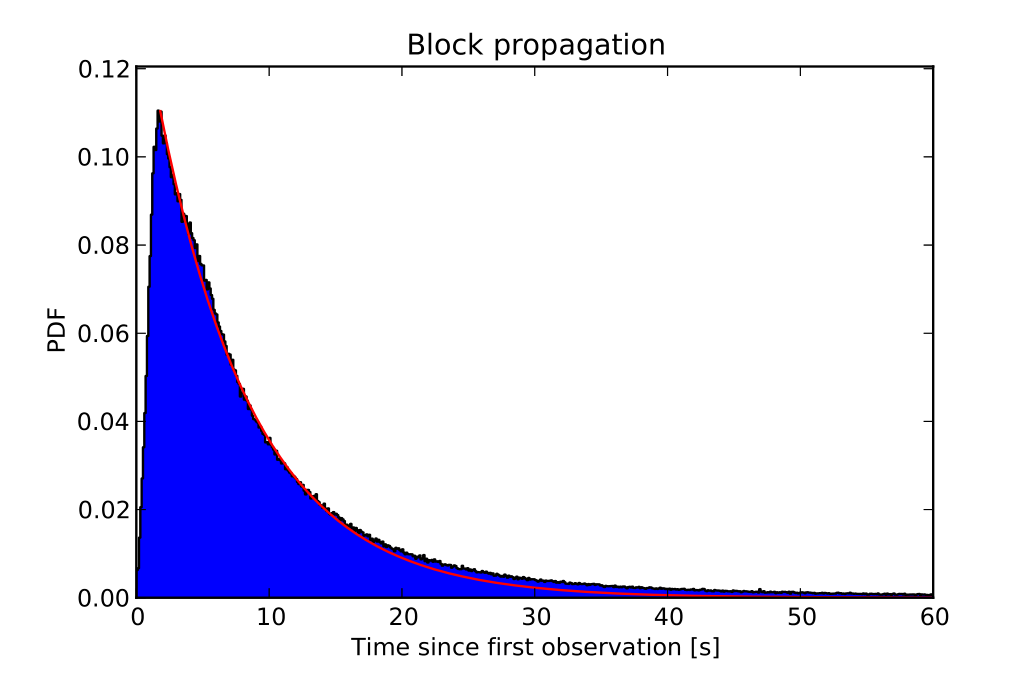
\includegraphics{bitcoinpropagation_3.PNG}
\caption{Istogramma normalizzato del tempo che intercorre dal primo annuncio del blocco con una curva di interpolazione esponenziale.\label{bitcoinpropagation_3}}
\end{figure}

Le misurazioni effettuate ci permettono di stabilire che il tempo mediano in cui un nodo riceve un blocco è di 6.5 secondi, mentre la media è di 12.6 secondi. La lunghezza della seconda fase, quella di contrazione esponenziale, evidenzia come dopo soli 40 secondi il 95\% dei nodi abbia ricevuto il blocco.

Abbiamo però detto come la dimensione di un blocco sia variabile, fino a 500kB. I dati precedenti sono aggregati per tutti i blocchi e non tengono conto delle differenti dimensioni degli stessi. Perciò definiamo ora il \emph{costo di ritardo} come il ritardo che ogni kB causa alla diffusione di una transazione o di un blocco. Tale costo risulta essere una combinazione sia del tempo di trasmissione che del tempo di verifica. I risultati sono contenuti nel grafico \ref{bitcoinpropagation_4}.

\begin{figure}[htbp]
\centering
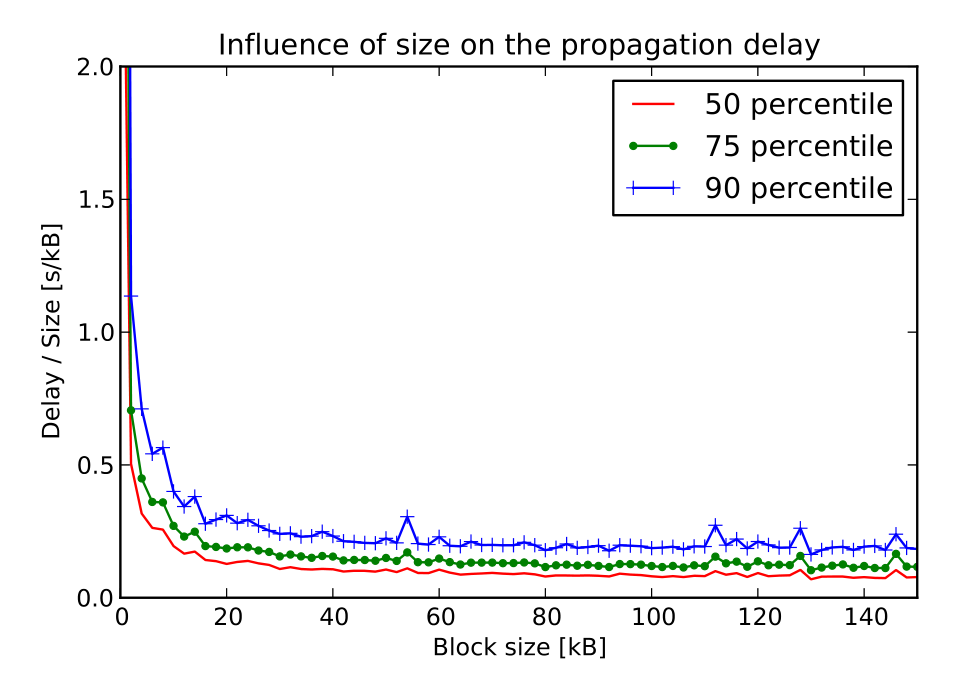
\includegraphics{bitcoinpropagation_4.PNG}
\caption{Costo del ritardo per il 50°, 75° e 90° percentile. Il grafico è focalizzato sui valori più bassi delle ascisse per poter mostrare il comportamento costante presente dopo i 20kB.\label{bitcoinpropagation_4}}
\end{figure}

%TODO tradurre roundtrip delay
Per pacchetti di dimensione superiore ai 20kB si vede come il costo sia pressoché costante, mentre per dimensioni minori si assiste a notevole ritardo. La causa di ciò sta nel \textbf{ritardo da un roundtrip}, ovvero il fatto che anche i piccoli messaggi vengono annunciati con \emph{inv} e richiesti con \emph{getdata}. Il roundtrip è dominante per le transazione in quanto il 96\% di tutte le transazioni sono inferiori ad 1kB. Per i blocchi, la cui dimensione è per la maggior parte superiore ai 20kB, ogni kB di dimensione costa circa 80ms di ritardo fino al momento in cui la maggioranza dei nodi non ha il blocco. %TODO verificare questa frase, sembra l'esatto opposto di quanto scritto nel grafico
Nel caso di piccoli blocchi sarebbe pertanto ottimale evitare l'annuncio e inoltrare direttamente il blocco ai nodi vicini.

\subsection{Informazioni scomparse}\label{informazioni-scomparse}

Trattiamo ora il caso in cui un blocco inoltrato in rete porti ad un fork della blockchain che viene rilevato solo da una piccola parte dei nodi.

Definiamo il grafo che descrive la rete come $G = (V,E)$, con $V$ i nodi (vertici) ed $E$ le connessioni tra i nodi (archi/edges). Definiamo inoltre la partizione $P_h \subset V$ come l'insieme dei nodi il cui blocco di testa si trova ad altezza $h$. Trovare un nuovo nodo $b_{h+1}$ crea una nuova partizione $P_{h+1,b}$ contenente i nodi che considerano questo nuovo blocco come blocco di testa, in altre parole questo è il primo blocco di altezza $h+1$ che abbiano ricevuto. Se non vengono trovati altri blocchi, allora i nodi di $P_h$ adiacenti a $P_{h+1,b}$ si uniscono a $P_{h+1,b}$ lasciando (e quindi eliminando) la partizione $P_h$. Dal'altro canto, se viene trovato un blocco $b'_{h+1}$ da un nodo in $P_h$ viene creata una nuova partizione $P_{h+1,b'}$. Anche in questo caso i nodi di $P_h$ abbandoneranno la loro partizione per unirsi ad una delle due nuove di altezza superiore. Solamente i nodi di $P_h$ che sono a contatto sia con $P_{h+1,b}$ che con $P_{h+1,b'}$ saranno consapevoli dell'esistenza di entrambe le partizioni e quindi del fork della blockchain, e considereranno invalido il blocco di altezza $h+1$ proveniente dall'altra partizione e di conseguenza non lo annunceranno ai loro vicini fermando quindi l'espansione della partizione. Tale meccanismo si applica anche alle transazioni: se due tx tentano di spendere lo stesso output, solo la prima transazione ricevuta da un nodo verrà considerata valida, la seconda verrà considerata invalida e non annunciata ai vicini. Questo comportamento ha il vantaggio di impedire ad un nodo malevolo di inondare la rete con centinaia di transazioni contraddittorie senza costo addizionale, in termini di transaction fees, per il nodo malevolo. Il rovescio della medaglia è che questo sistema di nascondere le informazioni ritenute sbagliate da un nodo permettere l'implementazione di \textbf{attacchi double spend} che risultano invisibili ai commercianti. Nel caso delle transazioni, dato che esse non devono per forza propagarsi a tutti i nodi, il meccanismo descritto è ragionevole e protegge la rete da transazioni spam. Nel caso dei blocchi invece, fermarne la propagazione è controproducente: i fork della blockchain, che con tale sistema sono invisibili per la maggior parte dei nodi, sono una cartina tornasole che indica come nella rete ci siano alcune inconsistenze non risolte. Dato che i blocchi valido ma potenzialmente in conflitto non possono essere creati con un frequenza arbitraria come le transazioni, permettere il loro inoltro anche nel caso di conflitto non crea possibilità per un potenziale attacco.

\section{Fork della blockchain}\label{fork-della-blockchain}

Durante il normale utilizzo della rete potrebbe capitare di essere testimoni di un fork se si ricevono due blocchi conflittuali, ma osservare tutti fork che avvengono è molto difficile a causa della non propagazione dei blocchi in conflitto discussa in precedenza. Se a questo aggiungiamo il fatto che una partizione potrebbe avere dimensione unitaria (un nodo genera un nuovo blocco in conflitto con il blocco di testa di tutti i suoi vicini) è evidente come per poter rilevare tutti i fork bisognerebbe connettersi ad ogni nodo della rete. Ma abbiamo detto che alcuni nodi non sono raggiungibili dall'esterno, per cui possiamo solo stimare il numero di fork che avvengono.

Utilizzando la configurazione descritta nella sezione precedente, sono stati raccolti tutti i blocchi di altezza compresa tra 180000 e 190000. Essendo un grande campione che coinvolge tutti i nodi raggiungibili, è abbastanza probabile che tutti i blocchi generati siano stati propagati fino al nodo spia implementato permettendo di individuare la maggior parte dei fork avvenuti nell'intervallo di rilevazione. Nei 10000 blocchi osservati sono stati identificati 169 fork, il che si traduce in rateo di forking $r = 1.69\%$. L'istogramma \ref{bitcoinpropagation_5} mostra i risultati in modo più dettagliato.

\begin{figure}[htbp]
\centering
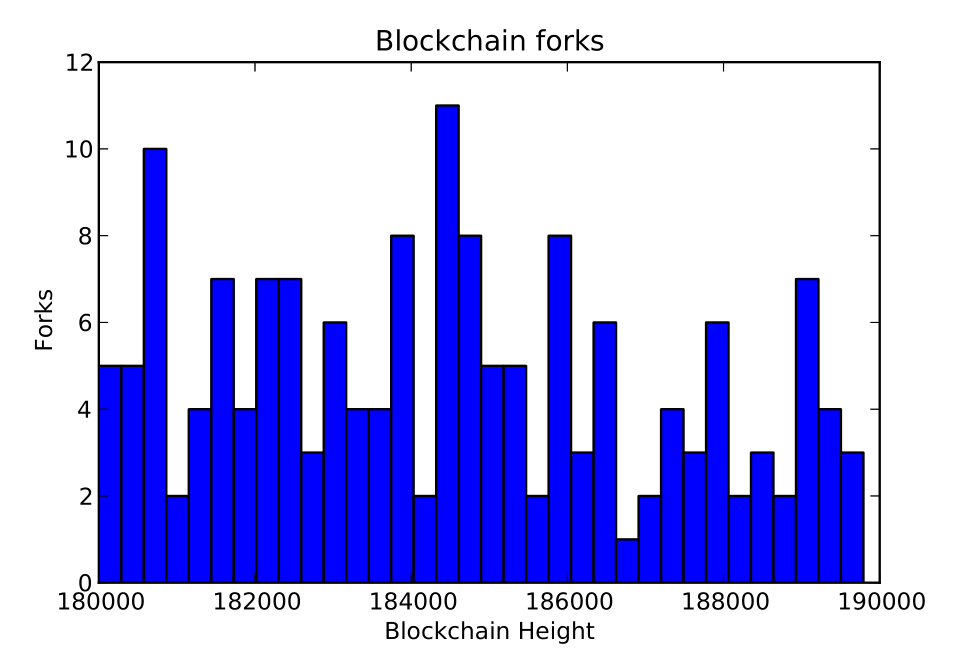
\includegraphics{bitcoinpropagation_5.PNG}
\caption{Fork osservati tra i blocchi 180000 e 190000 durante il collegamento alla rete.\label{bitcoinpropagation_5}}
\end{figure}

\subsection{Creazione del modello}\label{creazione-del-modello}

Il protocollo bitcoin adatta la difficoltà della proof-of-work ogni 10 minuti in modo da mantenerla sufficientemente elevata da essere significativa. Definendo $X_b$ come la variabile casuale che rappresenta i secondi trascorsi tra il ritrovamento di un nodo e il ritrovamento del nodo precedente, allora la \emph{probabilità che un blocco venga trovato} nella rete in un dato secondo è

\[ P_b = \Pr\left[ X_b < t + 1 | X_b \geq t\right] \approx 1/600 \]

Un fork avviene se, durante la propagazione del blocco $b$, viene trovato un blocco $b'$ in conflitto nella parte di rete non ancora a conoscenza di $b$. Definiamo $t_j$ come il tempo in secondi in cui $j$ apprende dell'esistenta di $b$ da quando esso è stato creato. La funzione $I_{j}(t)$ identifica se il nodo $j$ sa dell'esistenza di $b$ nell'istante $b$, e la funzione $I(t)$ conta il numero di nodi che hanno ricevuto e verificato $b$ all'istante $t$.

\[ I_{j}(t) = \begin{cases}
    0 &\textrm{se } t_j > t \\
    1 &\textrm{se } t_j \leq t
\end{cases}\]

\[ I(t) = \sum_{j \in V} I_{j}(t) \quad  \textrm{con }V\textrm{ insieme dei vettori} \]

Da cui ottengo il rateo di nodi informati:

\[ f(t) = \mathbb{E}[I(t)] \cdot n^{-1} \]

Notare come la $f(t)$ sia equivalente alla funzione di distribuzione cumulativa (\textbf{CDF}) della frequenza alla quale i peer vengono informati. Possiamo quindi utilizzare la funzione di densità di probabilità (\textbf{PDF}) della frequenza con cui i peer vengono informati rappresentata in \ref{bitcoinpropagation_3} come una approssimazione durante le rilevazioni. Solo i nodi non informati possono produrre blocchi in conflitto, per cui combinando la probabilità di trovare un blocco con il rateo di nodi non informati otteniamo la probabilità di un fork. Definiamo $F$ come la variabile casuale discreta che conta il numero di blocchi in conflitto trovati mentre un altro blocco viene propagato. Allora la propabilità di un fork risulta:

\[ \Pr\left[F \geq 1\right] = 1 - (1 - P_b)^{\int_{0}^{\infty} \! (1 - f(t)) \, \mathrm{d}t} \]

In questo ultimo passaggio si è assunta la semplificazione per la quale la probabilità di un nodo di trovare un blocco è distribuita uniformemente in modo casuale tra tutti i nodi.

Per cui, sapendo la probabilità dell'intera rete di trovare un blocco $P_b$ e la distribuzione di come i nodi apprendono dell'esistenza del blocco $I_j$, si può derivare la probabilità di un fork. Questi due valori dipendono dal potere computazionale della rete nonché dalla sua topologia e dimensione.

\subsection{Misurazioni}\label{misurazioni}

Per confermare il corretto funzionamento del modello proposto è necessario confrontare la probabilità ottenuta con i dati rilevati.

Bisogna innanzitutto notare come i nodi non sincronizzino i loro orologi interni, bensì si regolano sui loro vicini, esiste una differenza non trascurabile tra i timestamp. Ad esempio il blocco ad altezza 209873 ha un timestamp pari a 22:10:13 mentre il blocco ad altezza 209874 ha un timestamp di 22:08:44. Dato che il secondo include l'hash del primo, i blocchi sono stati trovati nell'ordine corretto. Da questo si deduce che il conflitto nei timestamp è derivato dalla mancata sincronizzazione degli orologi dei nodi.

%TODO il paragrafo seguente è scritto da cani.
%TODO scrivere che roba è un Processo di Poisson
In questa analisi si potrebbe tenere conto dell'orario in cui il nodo spia rileva l'annuncio del blocco e l'orario in cui il blocco è stato trovato. Anche se questo metodo non subisce la differenza di orario tra i nodi, potrebbe esistere un lieve ritardo tra il calcolo del blocco e la rilevazione del relativo annuncio, e per la misurazione abbiamo a disposizione solo il timestamp del blocco. Dato che il calcolo della proof-of-work è un processo di Poisson, la differenza temporale segue una distribuzione esponenziale. La combinazione della differenza temporale degli orologi e il tempo intercorso tra i ritrovamenti dei blocchi causa uno spostamento a destra del massimo. Possiamo correggere la situazione spostando a sinistra fin quando il massimo non risulta in $t=0$. L'orario di annuncio rilevato durante la misura non è influenzato dalla differenza temporale e produce l'istogramma corretto.

%TODO diagramma 6 pag 7 bitcoinpropagation

\[ g(t) = \lambda e^{-\lambda \cdot x}\]

Estraendo i timestamp dai blocchi tra altezza 180000 e 190000 si ottiene la distribuzione illustrata nel grafico \ref{bitcoinpropagation_6}. Interpolando la distribuzione ottenuta con la distribuzione esponenziale si ottiene $\lambda = 0.001578$ da cui risulta un tempo atteso tra due blocchi pari a $1 / \lambda = 633.68$ secondi. Interpolando la densità di probabilità del tempo tra i primi annunci e le misurazioni si ottiene $\lambda = 0.001576$ che si traduce in un tempo atteso tra due blocchi $1/ \lambda = 634.17$ secondi. Le due approssimazioni sono coerenti ma sono entrambe leggermente sopra il valore obiettivo di 600 secondi. La differenza è probabilmente dovuta ad un decremento del potere computazione della rete.

Per quando riguarda la propagazione dei nodi nella rete, a causa della normalizzazione il diagramma \ref{bitcoinpropagation_3} rappresenta anche la funzione di densità di probabilità (\textbf{PDF}) delle variabili casuali $t_{b,j}$ per tutti i blocchi $b$ dell'intervallo di misurazione. Per cui la frequenza dei nodi informati $f(t)$ è l'area che sottostà all'istogramma \ref{bitcoinpropagation_3} fino al tempo $t$.

\begin{figure}[htbp]
\centering
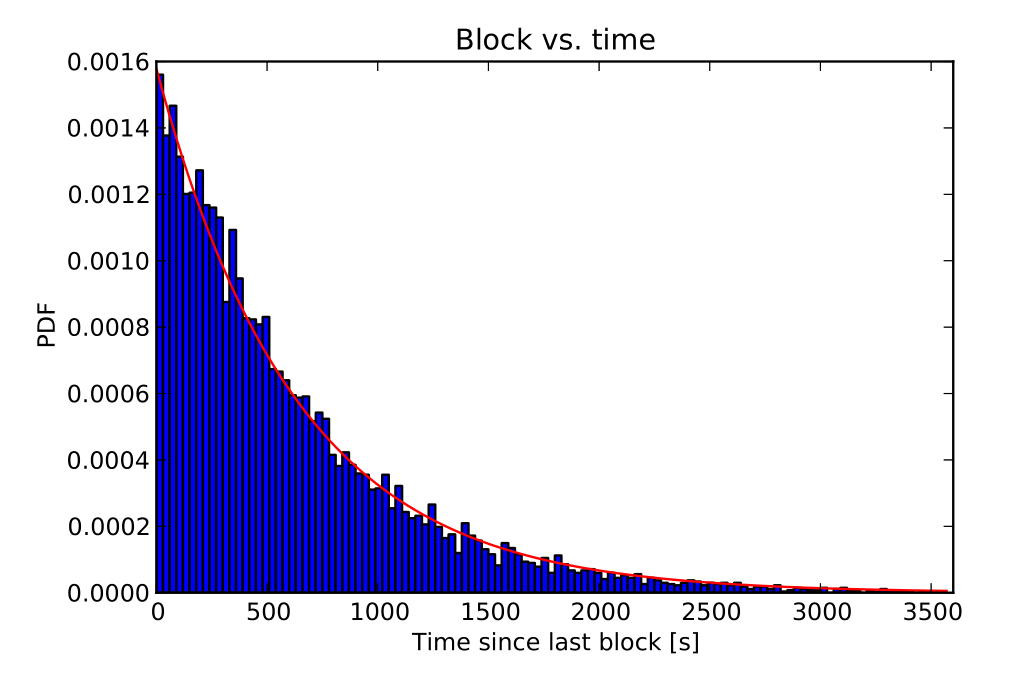
\includegraphics{bitcoinpropagation_6.PNG}
\caption{Tempo di distribuzione spostato a sinistra per i blocchi trovati tra le altezze 180000 e 190000.\label{bitcoinpropagation_6}}
\end{figure}

Combinando la probabilità di trovare un blocco e la funzione della frequenza dei nodi informati si ottiene la seguente probabilità per un fork:

\begin{equation}
\begin{aligned}
    \Pr [F \geq 1 ] &= 1 - (1 - P_b)^{\int_{0}^{\infty} \! (1 - f(t)) \, \mathrm{d}t} \\
    &= 1 - (1 - \frac{1}{633.68})^{11.37} \\
    &\approx 1.78%
\end{aligned}
\end{equation}

Comparando questo risultato con quello osservato di 1.69\% si nota di aver sovrastimato il valore osservato solo del 5\%. Il risultato leggermente superiore può essere spiegato dall'assunto fatto che la potenza di calcolo sia uniformemente distribuita tra tutti i nodi nella rete. Ciononostante, il buon risultato ottenuto dimostra come il modello sia una efficace rappresentazione della realtà.

Dato che il numero di transazioni e le dimensioni della rete molto probabilmente cresceranno mano a mano che aumenta l'adozione di Bitcoin, la frequenza dei fork è destinata a salire. Una rete più grande, con una topologia casuale e il numero di connessioni limitate per singolo nodo, aumenta il suo diametro e la distanza media tra i nodi e l'origine di un blocco. L'aumento del numero di transazioni provoca una crescita nella dimensione dei blocchi il che a sua volta aumenta il tempo necessario per la verifica e la trasmissione ad ogni passo della propagazione.

%TODO da qui in poi sono problematiche al metodo di propagazione. Sarebbe il caso di metterlo nel capitolo problemi e soluzioni

Una interpretazione alternativa del risultato proposto in %TODO link all'equazione precedente
è che ogni volta che un blocco viene trovato, l'equivalente di 11.37 secondi di potere computazionale dell'intera rete viene sprecato. Infatti il lavoro impiegato per trovare il primo blocco di una blockchain alternativa (che potrebbe essere scartata) non contribuisce alla sicurezza della rete e costituisce un eventuale punto a favore di un attaccante che cerca di implementare una sua blockchain alternativa. Come detto in precedenza da Nakamoto, un attaccante capace di controllare più del 50\% del potere computazione delle rete è in grado di trovare proof-of-work più velocemente di tutto il resto il della rete. L'attaccante sarebbe perciò in grado di rimpiazzare l'intera storia delle transazione a partire da un qualsiasi blocco. Pur sicuramente sufficiente, questa condizione non è minima. In realtà l'efficenza della rete come intero, incluso il ritardo di propagazione, non è ottimale. La potenza computazionale effettiva nella rete così come si presenta a Settembre 2013 è pari a $1 - 11.37 / 633.68 = 98.20\%$. Per cui ad un attaccante basta controllare il 49.1\% della forza di calcolo della rete per poter portare un attacco e cambiare la blockchain. Al momento questo è un risultato difficile da ottenere, ma la situazione potrebbe cambiare in peggio a causa dell'aumento costante del ritardo di propagazione.

\chapter{Privacy}\label{privacy}

Uno degli obiettivi del design di Bitcoin è l'anonimato dell'utente. Il paragone più appropriato è quello con i conti in banca della Svizzera. Ogni utente bitcoin può infatti possedere più di un portafogli (ovvero di una coppia di chiavi pubblica e privata) e per ogni portafogli più di un conto/indirizzo (che altro non è che una stringa unica generata grazia alla coppia di chiavi) e tutte le transazioni si basano unicamente sull'indirizzo. Non esiste quindi nessun modo per risalire al proprietario di un dato indirizzo bitcoin basandosi unicamente sulla struttura della rete.

Esistono ovviamente diverse tecniche sia per ridurre il livello di privacy, ad esempio tramite il furto delle chiavi o un'analisi statistica degli input e degli output delle transazioni, sia per aumentarlo, magari creando un diverso portafoglio per ogni conto che si desidera creare.

\section{Analisi quantitativa della privacy}\label{analisi-quantitativa-della-privacy}

Ma come si fa a misurare il livello di privacy offerto da Bitcoin? In questa sezione si discuteranno alcune metriche arbitrarie create appositamente che trattano i vari aspetti dell'anonimato nella rete Bitcoin.

Essendo una analisi quantitativa, è necessario fornire una definizione formale per i termini fin qui usati in modo più o meno descrittivo. Sotto tale ottica verrano quindi proposte alcune definizioni formali, la prima delle quali è il concetto portante della rete:

Transazione:
\[\tau(a_{\textrm{S}} \rightarrow a_{\textrm{R}}) = \{ \textrm{source}, B, a_{\textrm{R}}, \textrm{SIG}_{\textrm{sk}_{a_{\textrm{S}}}}(\textrm{source}, B, a_{\textrm{R}}) \} \]
definisce una transazione che intercorre tra i due indirizzi $a_{\textrm{S}}$ e $a_{\textrm{R}}$, in cui $\textrm{SIG}_{\textrm{sk}_{a_{\textrm{S}}}}$ è la firma digitale creata utilizzando la chiave privata $\textrm{sk}_{a_\textrm{S}}$ corrispondente alla chiave pubblica associata all'indirizzo $a_\textrm{S}$. $B$ è la quantità di BTC trasferite e $\textrm{source}$ è un riferimento alla più recente transazione da cui $a_\textrm{S}$ ha ottenuto le $B$ BTC.

Al fine dell'analisi, assumiamo la situazione tipica della rete Bitcoin, in cui ogni singolo utente dispone di diversi indirizzi a lui associati. Mentre questa può sembrare una forzatura, in realtà non lo è affatto. Come abbiamo detto in precedenza, ogni transazione contiene un indirizzo di ritorno per il resto. Tale indirizzo viene definito \emph{indirizzo ombra} ed è creato automaticamte senza l'intervento dell'utente. Per cui ogni utente possiede almeno due indirizzi: quello creato al momento della creazione del portafogli e l'indirizzo ombra.

\subsection{Il modello antagonistico}\label{il-modello-antagonistico}

Gli algoritmi proposti consistono nell'osservazione del log pubblico di Bitcoin (\emph{pubLog}) durante un periodo $\Delta t$. Durante questo periodo, $n_U $ utenti (dall'insieme $U = \{u_1, \ldots, u_{n_U}\}$) contribuiscono al \emph{pubLog} con l'insieme di indirizzi $A = \{a_1, \ldots, a_{n_A}\}$. Si ha poi l'insieme delle transazioni $T = \{ \tau_1 (S_1 \rightarrow R_1), \ldots , \tau_{n_T}(S_{n_T} \rightarrow R_{n_T}) \} $ in cui $\tau_i (S_i \rightarrow R_i)$ descrive una singola transazione con ID univoco pari a $i$, e con $S_i$ e $R_i$ l'insieme degli indirizzi di mittente e destinatario rispettivamente. Viene introdotto anche un avversario $\adversary$ interessato ad ottenere informazioni su tutte le transazioni e gli indirizzi appartenenti ad un insieme di utenti Bitcoin. Si assume quindi che $\adversary$ sia un nodo legittimo della rete, abbia accesso a \emph{pubLog}, ad alcuni indirizzi di commercianti resi pubblici e altre informazioni statistiche pubblicamente disponibili. Inoltre si assume anche che gli utenti siano incoraggiati a cambiare frequentemente i loro indirizzi, spostando le loro monete da un indirizzo all'altro. Questa è una delle abitudini consigliate da Nakamoto.

\subsection{Quantificazione della Privacy}\label{quantificazione-della-privacy}

Esistono (almeno) due nozioni distinte di privacy per la rete Bitcoin.

\emph{Activity unlinkability}: Un avversario $\adversary$ non dovrebbe essere in grado di associare due indirizzi distinti (\emph{address unlinkability}) o transazioni (\emph{transaction unlinkability}) ad un utente scelto dell'avversario stesso.

\emph{Profile indistinguishability}: L'avversario non deve essere in grado di ricostruire i profili (insieme di indirizzi e transazioni) di tutti gli utenti del \emph{pubLog}. Questa nozione di privacy è più forte della precedente, in quanto riguarda l'intera rete e non solo un utente. Inoltre i due profili (per transazioni e per indirizzi) non sono equivalenti quando si tratta di modellare il profilo di un utente, in quanto è possibile indovinare correttamente gli indirizzi di utenti coinvolti in poche transazioni ma sbagliare nel caso di pochi indirizzi coinvolti in molte transazioni.

Vengono definiti due algoritmi \emph{AddUnl} e \emph{ProfInd} che implementano una sorta di sfida in cui l'attaccante tenta di violare le due nozioni di privacy sopra descritte. Il risultato sarà una quantificazione delle nozioni di privacy nei termini del vantaggio che $\adversary$ possiede per vincere queste sfide nei confronti di un avversario $\adversaryrnd$ che tenta di vincere le stesse sfide rispondendo in modo casuale. Ipotizziamo che $\adversary$ abbia accesso completo a \emph{pubLog} e che sia $\adversary$ che $\adversaryrnd$ abbiano accesso ad una base di conoscenza comune $\knowa$ che contengono informazioni verificate su un sottoinsieme di indirizzi e i relativi proprietari.

\subsubsection{Address Unlinkability}\label{address-unlinkability}

Il seguente algoritmo descrive il meccanismo con cui avviene la sfida per la address unlinkability. In questo algoritmo si utilizza $\adversary$ come un generico avversario, in quanto per i calcoli di quantificazione l'algoritmo verrà eseguito sia da $\adversary$ che da $\adversaryrnd$. Si comincia con $\adversary$ che seleziona in modo causale un indirizzo presente in pubLog e lo invia ad uno sfidante $\challenger$ (che si assume sia a conoscenza delle corrette correlazioni utenti-indirizzi). Se l'indirizzo scelto da $\adversary$ è l'unico che appartiene all'utente, $\adversary$ vince la sfida. Altrimenti $\challenger$ scegli un bit casuale $\mathcol{b}$. Se $\mathcol{b} = 1$ allora $\challenger$ sceglie un nuovo indirizzo tra quelli disponibili in pubLog che appartenga allo stesso utente del primo indirizzo, altrimenti il nuovo indirizzo verrà scelto tra quelli in pubLog che non appartengono al proprietario del nuovo indirizzo. L'indirizzo scelto insieme al precedente indirizzo vengono inviati ad $\adversary$, il quale stima (con un algoritmo di sua scelta, ininfluente per la sfida) se i due indirizzi che ha ricevuto appartengono o meno allo stesso utente, e memorizza il suo risultato nel bit $\mathcol{b}'$. Se $\adversary$ ha indovinato, ovvero se $\mathcol{b} = \mathcol{b}'$, allora $\adversary$ vince la sfida. L'algoritmo è visibile in \ref{addunl_alg}.

\begin{algorithm}
	\caption{Address Unlinkability}
	\label{addunl_alg}
	\begin{algorithmic}
		AddUnl(A, \challenger, \knowa$, pubLog):
		\STATE $a_0 \leftarrow $A.randomAddr(pubLog)
		A.send($a_0, \challenger$)
		\IF{$\challenger$.isUniqueAddr($a_0$)
			A.win()
		\ELSE
			$\mathcol{b} \leftarrow \challenger$.randomBit()
			\IF{$\mathcol{b} = 1$}
				$a_1 \leftarrow \challenger$.sameUsrAddr($a_0$, pubLog)
			\ELSE
				$a_1 \leftarrow \challenger$.otherUsrAddr($a_0$, pubLog)
			\ENDIF
			$\challenger$.send($\langle a_0, a_1 \rangle$, A)
			$\mathcol{b}' \leftarrow $A.estimateSameUser($a_0, a_1$)
			\IF{$\mathcol{b} = \mathcol{b}'$} A.win() \ENDIF
		\ENDIF
	\end{algorithmic}
\end{algorithm}


Stabiliamo che Bitcoin soddisfa il principio di \emph{Address Unlinkability} se, per ogni avversario $\adversary$ (che ha un ben preciso algoritmo per rispondere alla domanda di $\challenger$) e per ogni coppia di indirizzi scelti dall'algoritmo, $\adversary$ ha solo un piccolo vantaggio rispetto ad un avversario come $\adversaryrnd$ che risponde a caso alla domanda posta da $\challenger$. Formalmente diciamo che Bitcoin soddisfa la Address Unlinkability se:

\[ Pr [ \mathcol{b}' \leftarrow \adversary (\text{pubLog}, \knowa ) : \mathcol{b} = \mathcol{b}' ] - \Pr [\mathcol{b}' \leftarrow \adversaryrn (\knowa) : \mathcol{b} = \mathcol{b}' ] \leq \varepsilon\]

con $\varepsilon$ trascurabile.

\paragraph{Quantificazione di Address Unlinkability}\label{quantificazione-di-address-unlinkability}

Sfruttando i risultati ottenuti dalla sfida, è possibile stimare il \emph{grado} con cui gli indirizzi Bitcoin possono essere collegati ad uno stesso utente. Verranno definite alcune strutture matematiche necessarie per i calcoli.

\[E_\text{link} [i, j] = \{p_{i,j}\}_{i,j \in [1, n_A ]}\]

Rappresenta una matrice $n_A \times n_A$ in cui ogni argomento esprime la probabilità $p_{i,j}$ stimata da $\adversary$ che l'indirizzo $a_i$ appartenga allo stesso utente dell'indirizzo $a_j$ (in simboli, $a_i \sameuser a_j$). Si definisce poi una matrice $n_A \times n_A$ che mantenga le informazioni sulle reali connessioni tra gli indirizzi:

\[\text{GT}_\text{link} [i,j] = \begin{cases} 1 &\text{se } a_i \sameuser a_j \\ 0 &\text{altrimenti} \end{cases}\]

Date queste due strutture, si definisce l'errore commesso da $\adversary$ nella sua stima come la \emph{distanza di Manhattan} che intercorre tra $E_\text{link} [i,*]$ e le vere associazioni di $a_i$ con tutti gli indirizzi in pubLog:

\[ \begin{align} \text{Er}_{\adversary} &= \| E_\text{link} [i, *] - \text{GT}_\text{link} [i,*]\|_1 \\ 
   &= \sum_x | E_\text{link} [i, x] - \text{GT}_\text{link} [i,x] | \quad \text{ con } x \in [1, n_A]
   \end{align}\]

Si può dunque determinare il successo di $\adversary$ per AddUnl come il massimo del suo errore:

\[ \begin{align} \text{Succ}_{\adversary} &= \max_{\forall a_i \not\in \knowa} (\| E_\text{link} [i, *] - \text{GT}_\text{link} [i,*]\|_1) \\
   &= \max_{\forall a_i \not\in \knowa}(\sum_x | E_\text{link} [i, x] - \text{GT}_\text{link} [i,x] |) \quad \text{ con } x \in [1, n_A]
   \end{align} \]

Stesse condizioni devono essere fatte per l'avversario con criterio di decisione casuale, $\adversaryrnd$. Mantenendo uguale $\text{GT}_\text{link} [i,j]$ è necessario definire la matrice $E^{\mathcol{R}}$\_come segue:

\[E^{\mathcol{R}}_\text{link} [i, j] = \begin{cases} \pi_{i,j} &\text{ se } \langle a_i, a_j \rangle \in \knowa \\ \rho + \rho(1-\rho)\tfrac{1}{2} &\text{ altrimenti} \end{cases}\]

Dove $\pi_{i,j}$ rappresenta la probabilità che gli indirizzi $a_i$ e $a_j$ appartengano allo stesso utente secondo $\knowa$, mentre $\rho$ è la frazione di indirizzi in $\{\text{pubLog} \smallsetminus \knowa\}$ che non può essere associata ad altri indirizzi (il che capita quando un utente ha solo un indirizzo)\footnote{l'esistenza degli indirizzi ombra   non ha al momento rilevanza, ma più avanti $\rho$ diventerà   trascurabile a causa della loro presenza.}. Per le coppie di indirizzi non incluse in $\knowa$ tale probabilità è $\rho + \rho(1-\rho)\tfrac{1}{2}$.

Le altre formule vengono mantenute uguali sostituendo $E^{\mathcol{R}}_\text{link} [i, j]$ a $E_\text{link} [i, j]$. Il grado di address unlinkability risulta quindi essere il grado di successo aggiuntivo che $\adversary$ può ottenere da pubLog in comparazione con $\adversaryrnd$, chiamato $Link^{\text{abs}}_{\adversary}$\footnote{(///FIXME:   non ho la minima idea di cosa sia la versione normalizzata)}.

\[ \begin{align} Link^{\text{abs}}_{\adversary} &= \text{Succ}_{\adversary} - \text{Succ}_{\adversaryrnd} \\
   &= \frac{\text{Succ}_{\adversary} - \text{Succ}_{\adversaryrnd}}{\text{Succ}_{\adversaryrnd}} \quad \text{ in versione normalizzata}
   \end{align}\]

\begin{itemize}
\itemsep1pt\parskip0pt\parsep0pt
\item
  an analisis of anonimity in bitcoin sistem
\end{itemize}

\chapter{Sicurezza}\label{sicurezza}

\section{Reti P2P in genere}\label{reti-p2p-in-genere}

Una rete di computer, di qualsiasi tipo essa sia, richiede    necessariamente un certo livello di sicurezza. Questo è ancora più vero per reti pubbliche in cui chiunque può inserirsi, come le reti P2P che
si appoggiano a Internet.
Tali reti sono un bersaglio particolarmente ghiotto per gli attaccanti proprio a causa della loro maggiore forza: il grande numero di utenti,
che equivale ad un grande numero di possibili bersagli. Ogni rete P2P deve quindi confrontarsi con la certezza che alcuni dei suoi nodi siano
malevoli.  Data la grande varietà di reti P2P, è necessario specificare cosa intendiamo per ``reti P2P in genere''. Il modello \cite{vulnerabilities} a cui si farà riferimento consiste nelle seguenti componenti di base:

\begin{itemize}
\itemsep1pt\parskip0pt\parsep0pt
\item
  Uno spazio degli ID composto da b bits.
\item
  Un sistema di mappatura degli ID.
\item
  Un sistema di routing, che utilizza una chiave per inoltrare un   messaggio alla sua destinazione. Questo include una serie di regole   per il churm.
\end{itemize}

%TODO vedere se usare la documentazione del prof per descrivere i modelli di rete P2P

Basandoci sul modello di rete OSI, classifichiamo gli attacchi come di basso, medio e alto livello, a seconda della vicinanza al livello di comunicazione fisico: più il livello dell'attacco è alto, più si basa sul software invece che sull'hardware.

Visto che le reti P2P sono costruite sulla base di altre reti, i livelli ISO/OSI a cui siamo interessati sono il livello applicativo (per il P2P vero e proprio) e il livello di comunicazione (per attacchi basati su TCP e IP).

\begin{figure}[htbp]
\centering
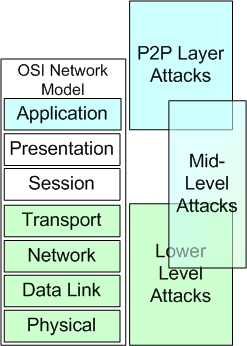
\includegraphics[width=\textwidth]{vulnerabilities_p2p-001.PNG}
\caption{Livelli di attacco in confronto con lo stack ISO/OSI.\label{vulnerabilities_p2p-001}}
\end{figure}

\subsection{Attacchi di Basso Livello}\label{attacchi-di-basso-livello}

\subsubsection{Denial of Service (DoS)}\label{denial-of-service-dos}

Uno degli attacchi più basilari che interessa praticamente ogni tipo di rete. Consiste nel bloccare i servizi offerti da uno specifico bersaglio. Si tratta di un attacco estremamente comune esistente in infinite varianti, ma nel caso di P2P la sua versione più semplice consiste nel flood. Consiste nell'estremizzare quanto descritto nel query flood\footnote{Confrontare sezione \ref{query-flooding}}: inondare la rete di pacchetti, legittimi o creati ad-hoc, in modo da ostacolare la normale comunicazione tra i nodi. Semplice, ma estremamente efficace.

Una variante ancora più efficace, e resa tale proprio dalla natura distribuita delle reti P2P, consiste nel \textbf{Distribute Denial of Service} (DDoS). Come dice il nome, la differenza sta nel fatto che l'attaccante non è un singolo nodo bensì un insieme di nodi. Il vantaggio in questa tecnica, oltre che nell'immenso numero di pacchetti che inondano la rete, sta nell'anonimato che circonda l'attaccante. Spesso infatti i nodi che a tutti gli effetti inviano i pacchetti sono inconsapevoli di essere parte dell'attacco e manipolati remotamente da un attaccante. Questo aggiunge un ulteriore strato tra l'attaccante e i nodi legittimi che tentano di impedire l'attacco.

Gli attacchi DoS e DDoS diventano tanto più probabili e quanto è vasta la rete, non solo per il maggior numero di nodi compromettibili per un DDoS, ma anche per le politiche aziendali attuate da molte società e provider. Infatti, più la rete è diffusa, più è probabile che firewall aziendali ne limitino l'accesso ai propri utenti e che ISP nazionali ne limitino l'utilizzo. Questo costringe gli utenti a piazzarsi al di fuori di tali reti protette per poter usufruire della rete P2P, e quindi ad esporsi maggiormente agli attacchi.

\paragraph{Contromisure al DDoS}\label{contromisure-al-ddos}

Il primo problema consiste nell'identificare i DDoS. I sintomi di un DDoS sono del tutto identici a quelli di un normale elevato traffico di rete, in particolare quando i pacchetti usati sono legittimi e non forgiati ad-hoc per l'attacco. Inoltre in un DDoS non tutti i nodi sono stati creati appositamente per attaccare, spesso sono nodi legittimi che vengono utilizzati dall'attaccante per far rimbalzare i suoi pacchetti di attacco. Questi due fattori combinati rendono di fatto \emph{impossibile} bloccare tutti gli attacchi DoS.

Esiste però una tecnica ampiamente diffusa per rendere poco pratico il DoS, o almeno per rallentarlo in maniera drastica. Si tratta del \textbf{pricing}, una tecnica che limita la velocità alla quale i nodi possono fare richieste alla rete. Se un nodo deve fare richieste ad un altro nodo (ad esempio, una query per un file), il nodo risponde con richieste di calcoli di hash, esattamente gli stessi calcoli necessari per creare un blocco in Bitcoin. Solo dopo aver risolto il calcolo ed inviata la risposta, la richiesta viene presa in considerazione, tutte le altre comunicazione inviate nel frattempo vengono scartate, scoraggiando quindi qualsiasi richiesta invadente.

\subsubsection{Attacco Man-in-the-Middle (MitM)}\label{attacco-man-in-the-middle-mitm}

Questo attacco consiste nell'inserimento dell'attaccante tra due nodi della rete, in modo che tutte le comunicazioni tra i due nodi passino attraverso l'attaccante. L'attacco è irrilevabile fin tanto che l'attaccante rimane passivo. Una volta ottenute tutte le informazioni che desidera, l'attacante può diventare attivo modificando i messaggi che vengono scambiati oppure forgiandone di propri spacciandosi per uno o entrambi dei nodi. Inoltre, dato che l'attacante può influenzare la visione che i due nodi hanno del resto della rete, può creare false identità per simulare messaggi legittimi.

Se questo attacco viene effettuato al livello di rete, l'attaccante è in grado di vedere tutto ciò che passa tra i due nodi e, essendo questo livello inferiore a quello P2P, l'attaccante non ha nessun problema nel creare qualsiasi tipo di pacchetto P2P egli desideri.

Come il DoS ma in misura estremamente maggiore, le reti P2P sono un bersaglio goloso per questo genere di attacchi. Questo perché è difficile inserirsi tra due nodi in una rete normale, ma in una rete P2P è estremamente banale: tali reti infatti non hanno nessun controllo su come sono localizzati i nodi e sono quindi \emph{estremamente} vulnerabili al MitM.
%TODO anche qui la stessa roba del tipo di reti del libro del prof
Dato che l'attaccante può piazzarsi dove vuole all'interno della rete, gli attacchi risultano essere molto specifici e deterministici, fino anche ad impedire ad un determinato nodo di accedere ad un altro nodo.

\subsubsection{Contrastare il Man-in-the-Middle}\label{contrastare-il-man-in-the-middle}

Il metodo principale per difendersi dal MitM è rendere tale attacco il più infruttuoso possibile. In una rete senza nodi privilegiati (ad esempio un server centrale, un supernodo o un'autorità centrale di autenticazione), il MitM si limita a compromettere la sicurezza tra due soli nodi nella rete, senza minacciare per nulla il resto dei nodi \footnote{almeno fino a quando la perdita di tre nodi (due vittime e un   attaccante) risulta tollerabile per la rete, il che è vero per tutte   quelle reti ampiamente diffuse.}.

Molte reti (non bitcoin) sfruttano nodi privilegiati per affrontare altre minacce o come parte integrante della loro struttura, e anche nelle reti maggiormente distribuite è possibile effettuare un attacco MitM su larga scala (vedi \ref{attacco-eclipse} più avanti).

Il metodo più diffuso per evitare la fuoriuscita di informazioni nella comunicazione tra due nodi è la cifratura a chiave pubblica. Con tale sistema si garantisce l'origine del messaggio, il fatto che non è stato alterato in alcun modo e, volendo, fornisce anche un metodo per evitare che una terza parte non autorizzata possa leggerne il contenuto. L'implementazione di questo semplice meccanismo rende praticamente inutile qualsiasi tentativo di MitM tra due nodi.

\subsection{Attacchi di Medio Livello}\label{attacchi-di-medio-livello}

\subsubsection{Worms}\label{worms}

Un worm è un programma auto-replicante simile a un virus che, a differenza di questo, è indipendente da altri programmi presenti sul sistema. La minaccia rappresentata da un worm è decisamente significativa per una rete P2P, in quanto si diffondono a tutti i nodi della rete tramite vulnerabilità presenti ad un livello più basso rispetto a quello della rete stessa. Pur non essendo legati direttamente al P2P, i worm vengono diffusi in modo capillare da esso principalmente a causa di come il P2P viene implementato. In molte architetture infatti i nodi per comunicare tra loro devono avere installato lo stesso software. Ciò significa che quando questo software ha una certa vulnerabilità (ad esempio, un buffer overflow), tutti i nodi della rete sono vulnerabili. Quindi mentre un worm ``normale'' deve effettuare una scansione dell'intera rete per trovare degli host vulnerabili, un worm P2P deve solo guardare le tabelle di routing e infettare tutti i nodi vicini, diffondendosi esponenzialmente: in confronto ai worm normali, i worm P2P infettano l'intera rete in modo praticamente istantaneo.

Oltre alla grande velocità di diffusione, il fatto che molte reti P2P siano concepite per il file-sharing e abbiano quindi una grande abbondanza di banda, consente al worm P2P di avere dimensioni maggiori e di essere quindi capace di azioni ed attacchi molto più complicati rispetto ad un worm normale, a volte grande solo come un pacchetto TCP/IP. Molti nodi sono inoltre spesso computer personali di utenti normali che utilizzano quotidianamente Internet. Worm sufficientemente complessi sono in grado di monitorare l'attività dell'utente anche al di fuori della rete P2P e di accedere a dati quali numero di carta di credito, password di account, ecc., rendendo le reti P2P un bersaglio di estremo valore.

Infine, i worm possono usare la rete come uno strumento. Si è parlato prima parlando del DDoS (nella sezione \ref{denial-of-service-dos}) di come un nodo qualsiasi possa diventare un ignaro vettore di attacco. I worm sono il modo in cui questo viene reso possibile: il worm contiene tutto il codice necessario ad effettuare l'attacco, oltre al codice per replicare se stesso negli altri nodi.

\paragraph{Contrastare i Worm}\label{contrastare-i-worm}

Il modo principale è mantenere le applicazioni sicure: senza una vulnerabilità comune un worm non può diffondersi in modo efficace. La sicurezza di un software dipende dal modo in cui esso è stato programmato, ad esempio per ridurre il rischio di buffer overflow è possibile usare linguaggi fortemente tipati.

Per ridurre invece l'efficacia di un worm si può decentralizzare il più possibile la rete evitando di implementare nodi privilegiati e/o utilizzare sistemi operativi \textbf{hardened}. OpenBSD dalla versione 3.8 per esempio utilizza indirizzi pseudocausali in fase di allocazione della memoria, rendendo quindi difficile sfruttare vulenrabilità presenti nei vari applicativi.

Ma il modo più pratico per difendersi dai worm è mantenere aperta la rete. Ciò significa basarsi su standard diffusi ed aperti per i propri applicativi. Rilasciare i protocolli al pubblico e distribuire il codice dei propri software incoraggia altri sviluppatori ad una analisi critica, il che porta alla più tempestiva scoperta di vulnerabilità ed alla rapida creazione di patch, bug-fix e fork più robusti del software in questione. Inoltre, con opportune licenze, ogni sviluppatore può creare il proprio client per interfacciarsi con la rete costringendo un attaccante a creare un worm specifico per ogni versione di ogni client, e a mantenere tale worm aggiornato mano a mano che nuove vulnerabilità vengono scoperte e risolte o nuovi client implementati. Con una grande varietà di client a disposizione, non tutti i nodi saranno vulnerabili allo stesso identico difetto presente in un altro client.

\subsection{Attacchi al livello P2P}\label{attacchi-al-livello-p2p}

\subsubsection{Comportamento scorretto}\label{comportamento-scorretto}
 Non si tratta di danneggiare una rete intera o un singolo nodo, bensì di trarre il massimo profitto offrendo minima collaborazione. Questo comportamento viene definito genericamente \textbf{attacco razionale}. La terminologia si basa sull'assunzione che dietro ogni nodo ci sia un utente razionale che per istinto tenta di trarre il massimo beneficio con il minimo sforzo. Ad esempio nell'ambito della rete BitTorrent un utente scarica un file eliminandolo dalla condivisione non appena completo, oppure riduce ai minimi termini la banda in upload massimizzando quella in download: tale comportamente viene definito significativamente \textbf{leeching}, letteralmente \emph{sanguisuga}.

Ci sono molte ragioni per cui un nodo debba comportarsi in questo modo:

\begin{itemize}
\itemsep1pt\parskip0pt\parsep0pt
\item
  Per preservare la banda in upload, spesso molto limitata dagli ISP.
\item
  Per motivi legali, in special modo dove la condivisione di contenuti   protetti dal copyright può risultare in un'azione legale nei confronti   del nodo che condivide. Data la natura aperta delle reti, spesso è   molto facile risalire all'origine di un contenuto.
\item
  Per istinto: molte persone, se viene lasciata loro possibilità di   scelta, tendono a non cooperare per il solo benificio di aiutare la   comunità a cui appartengono, non importa quanto minimo sia il costo   che comporta loro.
\end{itemize}

Come descritto, due sono i metodi in cui ci può implementare questo ``attacco'': riducendo le risorse a disposione della rete oppure riducendo il contenuto condiviso.

\paragraph{Contrastare i comportamenti scorretti}\label{contrastare-i-comportamenti-scorretti}

Ogni rete deve implementare il suo diverso meccanismo per favorire la collaborazione tra i peer: in Bitcoin ci sono le transaction fee, Napster utilizzava un meccanismo di reputazione che favoriva gli utenti che condividevano di più, Samsara (una rete di backup distribuito) consente ad un utente di utilizzare uno spazio su un altro nodo solo pari a quello che l'utente mette a disposizione per gli altri nodi.

Un esempio encomiabile è quello di BitTorrent: il protocollo è disinteressato al numero di file condivisi da un utente o dal contenuto di per se, ma si interessa solamente di quante risorse vengono condivise. Secondo il protocollo BitTorrent i file da condividere vengono suddivisi in parti (\textbf{chunks}) di lunghezza variabile che vengono barattati tra i nodi: più un nodo è disposto a dare, più si vedrà restituire. In pratica, più è alta la velocità di upload, più gli altri nodi assegneranno banda a quel nodo, aumentandone la velocità di download.

\subsubsection{Attacco Sibilla}\label{attacco-sibilla}

Si ha questo attacco quando una singola entità malevola rappresenta un grande numero (spesso estremamente elevato) di utenti in una rete P2P con l'obiettivo di assumere il controllo di un segmento della rete. L'attacco si implementa con l'attaccante che tenta di creare un grande numero dei nodi a lui vicini. L'attacco diventa più efficace se l'attaccante è in grado di decidere dove posizionarsi nella rete, in quanto potrebbe aver bisogno di meno nodi per poter causare gravi danni alla rete. Con molti nodi a propria disposizione è possibile controllare tutti i messaggi che passano per il segmente formato dai nodi in questione. Questo attacco è inoltre un \textbf{attacco gateway}, il che sta ad indicare una categoria di attacchi solitamente usati come passo preliminare per attacchi su vasta scala di altro tipo, come per esempio l'attacco Eclipse descritto nella sezione \ref{attacco-eclipse}.

\paragraph{Contromisure all'attacco Sibilla}\label{contromisure-allattacco-sibilla}

La natura aperta delle reti P2P gioca a favore di questo tipo di attacco: senza un'autorità centrale è impossibile fermare completamente un attacco Sibilla. Il meglio che si può fare è renderlo impraticabile.

Per rallentare un attacco si può usare lo stesso metodo usato con gli attacchi DoS: il pricing (confrontare la sezione \ref{denial-of-service-dos}).
Il grande numero di calcoli richiesti per unire molti nodi alla rete può richiedere all'attaccante più tempo di quanto sia disposto ad impiegarne. Se inoltre la rete implementa una sorta di tempo massimo durante il quale un nodo mantiene un certo identificativo, tutti gli attacchi hanno un tempo massimo entro il quale devono essere portati a termine, dopo di che i nodi creati dovranno ricollegarsi alla rete e quindi si dovranno ripetere tutte le pratiche del pricing.

\subsubsection{Attacco Eclipse}\label{attacco-eclipse}

L'obiettivo di questo attacco è di separare la rete in due o più partizioni. Quando l'attacco ha successo, tutte le comunicazioni tra le due partizioni devono passare attraverso un singolo nodo malevolo. In pratica questo risulta in un attacco Man-in-the-Middle su vasta scala eseguito a livello applicativo e non a livello di rete, con tutte le potenzialità del MitM normale. Per eseguire l'attacco bisogna piazzare i propri nodi in punti di routing strategici che esistono tra le due partizioni che si vogliono creare. Un attacco Eclipse di successo può distruggere qualsiasi rete P2P, soprattutto quelle che non si curano molto di mantenere tabelle di routing efficienti, perché i nodi finti possono essere posizionati in modo da riempire i vuoti nelle tabelle di routing di ogni altro nodo.

\paragraph{Contromisure ad Eclipse}\label{contromisure-ad-eclipse}

Data la similarità di Eclipse con il MitM, le contromisure sono anche similari: cifratura a chiave pubblica. Tuttavia, sebbene MitM non sia una minaccia per la rete, le dimensioni di Eclipse lo rendono estremamente pericoloso anche in caso di cifratura a chiave pubblica. Se i messaggi illeciti indirizzati ai nodi legittimi vengono bloccati, le due partizioni create da Eclipse rimangono di fatto isolate. Con abbastanza nodi piazzati in punti strategici della rete, è possibile creare quante divisioni si desidera, riducendo quindi le dimensioni della rete.

Come per l'attacco Sibilla, è importante impedire ad un attaccante di decidere dove piazzare i suoi nodi. Questo significa che sarà richiesto un elevato numero di nodi per avere una speranza di ottenere sufficiente controllo per poter creare una partizione. Per cui è importante notare che con un attacco Sibilla sufficiente grande è \emph{sempre} possibile eseguire un attacco Eclipse.

\subsection{Contromisure generali}\label{contromisure-generali}

Si è quindi visto come, oltre alle caratteristiche di tolleranza ai guasti e grande scalabilità che ne rappresentano la base del design, le reti P2P devono anche essere progettate per difendersi dagli attacchi. Solo in questo modo una rete potrà consentire ad ogni nodo di collegarsi e realizzare in pieno il concetto di collaborazione che sta alla base.

In particolare i progettisti di reti P2P dovrebbero implementare le seguenti caratteristiche:

\begin{itemize}
\itemsep1pt\parskip0pt\parsep0pt
\item
  L'impossibilità per un nodo di decidere in che punto della rete   piazzarsi.
\item
  Un limite per la velocità di churm per i nuovi nodi.
\item
  Limitare la velocità di scambio di messaggi tra i nodi, ad esemppio   con un princing.
\item
  Utilizzare la crittografia a chiave pubblica per garantire solo   messaggi legittimi tra i nodi.
\item
  Usare ed implementare solo standard aperti, per diversificare il   software a disposizione degli utenti ed irrobustire quelli esistenti.
\end{itemize}

Se queste caratteristiche vengono implementate, allora tutti gli attacchi fin qui descritti perdono gran parte della loro efficacia, ripagando con la sicurezza il costo che richiede la loro realizzazione.

\section{La rete Bitcoin; attacchi doppia-spesa}\label{la-rete-bitcoin}

\subsection{Attacchi basati sulla velocità}\label{double-spending}

Come descritto dallo stesso autore in \cite{bitcoin}, una transazione Bitcoin viene fissa nella blockchain e quindi resa (tecnicamente \ref{attacchi-hashrate}) immutabile solamente quando inclusa in un blocco. Dato che la rete si autoregola per trovare un blocco ogni 10 minuti circa, è evidente come questo sia il tempo minimo di attesa da lasciar trascorrere di avere la certezza che una transazione sia andata a buon fine. Questo meccanismo di verifica è eccellente per commerci in cui la consegna del servizio è dilazionata nel tempo rispetto al pagamento, come ad esempio il caso dell'acquisto online, ma risulta inefficace nel caso in cui la consegna del servizio richiesto sia rapida, nell'ordine dei 30 secondi: mentre l'attesa è un problema personale, la mancata conferma del buon esito della transazione espone il commerciante al rischio di non ricevere il pagamento subendo un attacco doppia-spesa. Con il termine \emph{doppia-spesa} ci si riferisce al caso in cui un utente $\mathcal{A}$ può reclamare la proprietà e spendere presso un diverso indirizzo le stesse BTC precedentemente inviate all'indirizzo di un venditore $\mathcal{V}$ in cambio di servizi che non vengono quindi retribuiti.\\
Karame, Androulaki e Capkun, nella loro ricerca \cite{doublespendig_fast} hanno analizzato il problema da un punto di vista formale evidenziandone le criticità e proponendone alcune soluzioni, in aggiunta ai consigli che gli stessi sviluppatori, ben consapevoli del problema, forniscono ai venditori che intendono usare Bitcoin per pagamenti rapidi.
La prima cosa che i ricercatori fanno notare è che sebbene i tempi di conferma delle transazioni in Bitcoin siano modellabili come una distribuzione geometrica traslata a sinistra(\ref{misurazioni}) in cui i tempi di conferma medi siano intorno ai 10 minuti, la deviazione standard raggiunge i 15 minuti: tali misurazioni sono basate sui primi 153260 blocchi (fino al 14 Novembre 2011) che mostrano inoltre come solo il 64\% di quei blocchi sia stato generato in meno di 10 minuti, mentre per il rimanente 36\% sono stati necessari tra i 10 e 40 minuti. Come si vede, il problema è rilevante per gli scambi commerciali che devono per forza di cose essere molto rapidi.

\subsubsection{Modello di attacco}

Come accennato, si considera il caso in cui un attaccante/acquirente $\mathcal{A}$ desideri ottenere un servizio rapido da un venditore $\mathcal{V}$ senza spendere le proprie BTC, ovvero facendo credere a $\mathcal{V}$ di essere stato pagato salvo poi deviare il pagamento verso un altro indirizzo impedendo a $\mathcal{V}$ di reclamare le BTC che gli spettano.\\
Si immagini quindi che $\mathcal{A}$ crei una transazione $\tau_\mathcal{V}$ diretta a $\mathcal{V}$ ed entro pochissimi secondi crei una seconda transazione $\tau_\mathcal{A}$ che sfrutti lo stesso identico input della precedente ma che come destinatario abbia un indirizzo sotto il controllo di $\mathcal{A}$. Quando $\mathcal{V}$ riceve la prima transazione, cosa che richiede mediamente 3 secondi, nel suo client può verificare come l'indirizzo del mittente e l'ammontare siano corretti e fornire quindi il servizio richiesto. Ma ad essere confermata tramite l'inclusione in un blocco sarà la seconda $\tau_\mathcal{A}$ che impedirà in modo irreversibile a $\mathcal{V}$ di ricevere il suo pagamento. Infatti se le due transazioni vengono inviate molto vicine nel tempo, solamente una di esse verrà inclusa in un blocco in quanto i nodi considerano invalide transazioni che hanno lo stesso input di transazioni precedentemente ricevute.\\
Impostando $\mathcal{X} \in \left[ \mathcal{A}, \mathcal{V} \right]$ e denotando con $t^\mathcal{X}_i$ l'istante in cui il nodo $i$ riceve $\tau_\mathcal{X}$ e con $t^\mathcal{X}_\mathcal{V}$ l'istante in cui $\mathcal{V}$ riceve $\tau_\mathcal{X}$ si hanno due condizioni necessarie da rispettare per un attacco doppia-spesa di successo. Ovviamente questi requisiti sono sufficienti solo nel caso in cui il commerciante verifichi solamente la ricezione della transazione sul proprio client e non sfrutti altre tecniche per verificare od eliminare gli attacchi doppia-spesa. Mentre queste assunzioni rispecchiano le attuali implementazioni dei client, non tengono conto dei consigli dati a coloro che intendono aprire un'attività commerciale Bitcoin basata sui pagamenti rapidi, che verranno descritti più avanti.

\paragraph{1: $t^\mathcal{V}_\mathcal{V} < t^\mathcal{A}_\mathcal{V}$}

Se tale requisito non viene rispettato allora $\mathcal{V}$ riceverebbe prima $\tau_\mathcal{A}$ rifiutando $\tau_\mathcal{V}$ e quindi richiedendo a $\mathcal{A}$ un nuovo pagamento o rifiutandosi di offrire il servizio.\\
$\mathcal{A}$ tenta quindi di connettersi direttamente ad uno dei nodi di $\mathcal{V}$\footnote{Gli indirizzi IP di un commerciante vengono infatti solitamente resi pubblici, in quanto sfruttabili per le transazioni al posto degli indirizzi Bitcoin.}: le specifiche del protocollo autorizzano sempre la connessione se non è stato raggiunto il numero massimo consentito (di default impostato a 125) di connessioni in ingresso. Si assuma inoltre che $\mathcal{A}$ abbia a disposizione uno o più nodi aiutanti denotati come $\mathcal{H}$\footnote{Possono essere processi sulla stessa macchina di $\mathcal{A}$, non è rilevante.} con i quali la comunicazione è dedicata e che non si connettono mai a $\mathcal{V}$. Con questo setup predisposto, $\mathcal{A}$ invia $\tau_\mathcal{V}$ a $\mathcal{V}$ nell'instante $t_\mathcal{V}$ e $\tau_\mathcal{A}$ ad $\mathcal{H}$ nell'instante $t_\mathcal{A} = t_\mathcal{V} + \Delta t$. Sia $\delta t^\mathcal{A}_\mathcal{HV}$ il tempo che impiega $\tau_\mathcal{A}$ a propagarsi da $\mathcal{H}$ a $\mathcal{V}$ e $\delta t^\mathcal{V}_\mathcal{AV}$ il tempo che impiega $\tau_\mathcal{V}$ a propagarsi da $\mathcal{A}$ a $\mathcal{V}$. In tal caso si ha la seguente stima:
\begin{align*}
t^\mathcal{A}_\mathcal{V} - t^\mathcal{V}_\mathcal{V} &\approx \tau_\mathcal{A} + \delta t^\mathcal{A}_\mathcal{HV} - \left( \tau_\mathcal{V} + \delta t^\mathcal{V}_\mathcal{AV} \right) \\
&\approx \Delta t + \delta t^\mathcal{A}_\mathcal{HV} - \delta t^\mathcal{V}_\mathcal{AV}
\end{align*}

Dato che, a differenza di $\mathcal{A}$ che lo è sempre, $\mathcal{H}$ non sarà mai vicino ad $\mathcal{V}$, si ha $\delta t^\mathcal{A}_\mathcal{HV} \geq \delta t^\mathcal{V}_\mathcal{AV}$ il che suggerisce $t^\mathcal{V}_\mathcal{V} < t^\mathcal{A}_\mathcal{V}$ per un qualche appropriato $\Delta t \geq 0$.

\paragraph{2: $\tau_\mathcal{A}$ confermata nella blockchain}

Nel caso in cui venga confermata $\tau_\mathcal{V}$, $\mathcal{A}$ non avrebbe più modo di riappropriarsi delle sue BTC.\\
È quindi necessario stimare le probabilità che ha $\tau_\mathcal{A}$ di essere inclusa in un blocco per prima partendo dall'istante $t_0$ in cui entrambe le transazioni coesistono nella rete ma non sono state incluse in un blocco.
Per far ciò si divida il tempo in eguali intervalli di ampiezza $\delta t$ tale che la probabilità di generare un blocco in ogni intervallo sia una sfida di Bernoulli con probabilità di successo $np$, dove $n$ è il numero di peer e $p$ è la probabilità di successo che ha un peer nel generare un blocco nell'intervallo $\delta t$. Sia $n^k_\mathcal{X}$ il numero di peer che hanno ricevuto $\tau_\mathcal{X}$ entro il tempo $t_k = k \delta t + t_0$, allora la probabilità che $\tau_\mathcal{X}$ sia inclusa in un blocco generato nell'intervallo $\left( t_k , t_{k+1} \right]$ è
\[P^k_\mathcal{X} = n^k_\mathcal{X} p \]
La probabilità che un blocco contenente $\tau_\mathcal{X}$ sia generato nello stesso intervallo è

\[ \textrm{p}_\mathcal{X}(k) = P^k_\mathcal{X} \prod^{k-1}_{i=0} \left(1 - P^i_\mathcal{X} \right) = n^k_\mathcal{X} p \prod^{k-1}_{i=0} \left(1 - n^i_\mathcal{X} p \right)  \]

Se all'istante $t_s = s \delta t + t_0$ ogni nodo della rete ha ricevuto almeno una delle transazioni $\tau_\mathcal{X}$, vale la seguente:

\[
\begin{cases}
  n^k_\mathcal{X} \leq n^{k+1}_\mathcal{X} &\textrm{ se } k < s \\
  n^k_\mathcal{X} = n^{k+1}_\mathcal{X} = n^s_\mathcal{X} &\textrm{ altrimenti}
\end{cases}
\]

Il che suggerisce $\forall i \geq s, n^i_\mathcal{V} + n^i_\mathcal{A} = n^{k+1}_\mathcal{V} = n^s_\mathcal{V}$.
Con l'assunto che $\forall k , n^k_\mathcal{X}$ non si scambiano i blocchi appena costruiti, i temp $t_{g_\mathcal{X}}$ necessari perché i nodi che lavorano in favore di $\tau_\mathcal{X}$ generino un blocco sono tra loro indipendenti, il che porta la probabilità che il requisito sia soddisfatto ad essere:

\[ P^{\left(2\right)}_S = \Pr \left( t_{g_\mathcal{A}} < t_{g_\mathcal{V}} \right) + \frac{1}{2}\Pr \left( t_{g_\mathcal{A}} = t_{g_\mathcal{V}} \right) \]

dove

\begin{align*}
\Pr \left( t_{g_\mathcal{A}} < t_{g_\mathcal{V}} \right) &= \sum^{\infty}_{g_\mathcal{A} = 0} \textrm{p}_\mathcal{A}\left(g_\mathcal{A}\right)\textrm{p}_\mathcal{V}\left(g_\mathcal{V} > g_\mathcal{A} \mid g_\mathcal{A} \right) \\
&= n^0_\mathcal{A}p\left(1 - n^0_\mathcal{V}p \right) + \sum^{\infty}_{g_\mathcal{A} = 0} \left( n^{g_\mathcal{A}}_\mathcal{A} p \left( 1 - n^{g_\mathcal{A}}_\mathcal{V} p \right) \prod^{g_\mathcal{A} -1}_{j=0} \left( 1 - n^j_\mathcal{V} p \right) \left(1 - n^j_\mathcal{A} p \right) \right)
\end{align*}

corrisponde all'evento in cui il blocco contenente $\tau_\mathcal{A}$ è il primo ad essere generato, e

\[ \Pr \left( t_{g_\mathcal{A}} = t_{g_\mathcal{V}} \right) = \sum^{\infty}_{g_\mathcal{A}=1} \left( p^2 n^{g_\mathcal{A}}_\mathcal{V} n^{g_\mathcal{A}}_\mathcal{A} \prod^{g_\mathcal{A} - 1}_{j=0} \left( 1 - n^j_\mathcal{V} p \right)\left( 1 - n^j_\mathcal{A} p \right) \right) \]

è l'evento in cui i due blocchi contenenti $\tau_\mathcal{A}$ e $\tau_\mathcal{V}$ sono generati nello stesso istante $t_{g_\mathcal{A}} = t_{g_\mathcal{V}}$. In quest'ultimo caso, la probabilità che il blocco contenente $\tau_\mathcal{A}$ venga adottato nella blockchain è $\frac{1}{2}$.

Androulaki, Karame e Capkun hanno testato $P^{\left(2\right)}_S$ per diversi valori di $n^k_\mathcal{X}$ e $p$ con $t_s = \delta t = 10$ secondi e 60000 nodi. Da tale analisi (visibile in forma completa nell'appendice B di \cite{doublespendig_fast}) risulta che $\mathcal{A}$ può massimizzare $P^{\left(2\right)}_S$ incrementando il numero di peer che riceveranno $\tau_\mathcal{A}, n^k_\mathcal{A} \forall t_k$. Ciò è fattibile inviando $\tau_\mathcal{A}$ prima di $\tau_\mathcal{V}$ e/o aumentare il numero di aiutanti. Nel caso decida di inviare la propria transazione fraudolenta prima di quella legittima, il ritardo con cui può trasmettere $\tau_\mathcal{V}$ rispetto ad $\tau_\mathcal{A}$ può essere al massimo $\Delta t = \delta t^\mathcal{A}_\mathcal{HV} - \delta t^\mathcal{V}_\mathcal{AV}$.

\subsubsection{Risultati sperimentali}

Denotando con $P^{\left(1\right)}_S$ la probabilità che il primo requisito sia soddisfatto, la probabilità totale di riuscita dell'attacco è $P_S = P^{\left(1\right)}_S P^{\left(2\right)}_S$.\\
I ricercatori hanno poi creato una rete Bitcoin ad-hoc distribuita in un'ampia area geografica per testare sperimentalmente i loro risultati con una configurazione ispirata a quanto riportato nella sezione precedente. I risultati visibili nel dettaglio in \cite{doublespendig_fast} mostra come la probabilità di successo di $\mathcal{A}$ non siano trascurabili. Anche se, in conformità con l'analisi, $\P_S$ è inversamente proporzionale a $\Delta t$ a causa dell'aumentato numero di peer che ricevono $\tau_\mathcal{V}$, per valori molto alti di $\Delta t$ (2 secondi) bastano 2 aiutanti per raggiungere percentuali di successo superiori al 90\% e, con lo stesso numero di aiutanti ma $\Delta t = 1$ secondi il successo dell'attacco è garantito.\\
Si è notato come il numero delle connessioni di $\mathcal{V}$ sia di importanza fondamentale per il risultato di $P_S$, soprattutto nel caso in cui $\mathcal{A}$ controlli un numero ristretto di aiutanti: nel caso in cui il numero di connessioni di $\mathcal{V}$ si avvicini al numero di $\mathcal{H}$ la probabilità di successo $P_S$ si avvicina a $\frac{1}{2}$, il che corrisponde al caso in cui $\tau_\mathcal{V}$ e $\tau_\mathcal{A}$ siano egualmente distribuite nella rete.

\subsubsection{Prevenire la doppia-spesa in velocità}\label{prevenzione-doppia-spesa}

\paragraph{Periodo di sorveglianza}

Dato che il demone Bitcoin genera un errore nel caso in cui riceva due diverse transazioni con lo stesso input\footnote{Anche se tale errore non viene normalmente mostrato all'utente}, un venditore accorto può subito individuare un tentativo di doppia spesa: aspettando pochi secondi prima di fornire i propri servizi ad $\mathcal{A}$, $\mathcal{V}$ può impiegare tale tempo monitorando tutte le transazioni che riceve il proprio client ed evitare quindi di incorrere in spiacevoli sorprese.\\
Purtroppo però questo regime di sorveglianza può risultare inefficace se $\mathcal{A}$ calcola meticolosamente i tempi di inoltro delle sue transazioni, ritardando l'invio di $\tau_\mathcal{A}$ di un tempo $t=\left(t^\mathcal{A}_\mathcal{V} - t^\mathcal{V}_\mathcal{V}\right)$ eccedente il periodo di monitoraggio mantenendo alte le probabilità di diffondere $\tau_\mathcal{A}$ nella rete. Ovviamente all'aumentare di $t$ aumenta anche la diffusione di $\tau_\mathcal{V}$, per cui $\mathcal{A}$ dovrebbe anche aumentare il numero $N_\mathcal{H}$ di $\mathcal{H}$ per mantenere soddisfacenti le proprietà probabilità di riuscita. Androulaki, Karame e Capkun hanno tentato di trovare la tripletta $\left( \Delta t, N_\mathcal{H}, C \right)$ (con $C$ il numero di connessioni di $\mathcal{V}$ ) tale che la probabilità $P_D$ che $\mathcal{V}$ riceva $\tau_\mathcal{A}$ dopo aver ricevuto $\tau_\mathcal{V}$ sia minimizzata. La loro analisi mostra come esista di fatto per $C < 80$ un periodo $\Delta t$ tale che $P_S \geq P_D$, il che significa che esiste effettivamente la possibilità per $\mathcal{A}$ di aggirare i controlli di $\mathcal{V}$ nel caso in cui questi utilizzi un periodo di monitoraggio e portare comunque a termine il suo attacco. È inoltre importante notare che anche quando la probabilità di successo risulta molto scarsa, se $P_D$ è anch'essa bassa $\mathcal{A}$ ha ottime ragioni per tentare lo stesso di portare il suo attacco, dato che sarà difficilmente individuato. I risultati mostrano inoltre l'esistenza di una $\left( \Delta t, N_\mathcal{H}, C\right)$ tale che $t = \infty$, ovvero il caso in cui tutti i vicini di $\mathcal{V}$ ricevono $\tau_\mathcal{V}$ come prima transazione non inoltrando $\tau_\mathcal{A}$ a $\mathcal{V}$ il quale non può quindi accorgersi del comportamento scorretto di $\mathcal{A}$ da cui consegue $P_D = 0$.\\\\
Risulta quindi fondamentale il numero di connessioni di $\mathcal{V}$: con pochi vicini aumentano le probabilità che tutti essi ricevano $\tau_\mathcal{V}$ prima di $\tau_\mathcal{A}$ considerando quindi invalida (giustamente) la transazione fraudolenta, non inviandola di conseguenza a $\mathcal{V}$ il quale non si accorge dell'attacco in corso che può benissimo andare a termine se $\tau_\mathcal{A}$ viene confermata nella blockchain. La tecnica di monitoraggio diventa tanto più efficace quanto maggiore è il numero di connessioni che $\mathcal{V}$ mantiene attive e tanto maggiore è la durata del periodo di monitoraggio (ovviamente nei limiti di quelle che sono considerate transazioni rapide, ad esempio 15 secondi).

\paragraph{Sorveglianti in rete}

Una soluzione similare alla metodologia d'attacco proposta vede $\mathcal{V}$ schierare in campo l'equivalente degli aiutanti $\mathcal{H}$ di $\mathcal{A}$, ovvero dei sorveglianti che inoltrino direttamente a $\mathcal{V}$ tutte le transazioni che ricevono: in tal modo egli sarà consapevole di eventuali transazioni $\tau_\mathcal{A}$ entro pochi secondi indipendentemente che tale transazione sia stata ricevuta da lui o da uno dei suoi sorveglianti. Risultati sperimentali mostrano come con soli 5 sorveglianti tutti i tentativi di doppia spesa siano stati individuati entro pochi secondi. È però da far presente come, dato il ritardo con cui $\mathcal{A}$ ha inviata $\tau_\mathcal{A}$, solo una piccola parte dei sorveglianti abbia ricevuto tale transazione prima di $\tau_\mathcal{V}$, permettendo quindi l'individuazione dell'attacco.\\
Come nel caso delle connessioni è evidente come il numero di sorveglianti faccia la differenza: utilizzare circa 3 sorveglianti ognuno dei quali con moltissime connessioni a nodi diversi da quelli degli altri sorveglianti possa intercettare efficacemente questo tipo di attacchi.

\paragraph{Collaborazioni tra i peer}

Un contromisura efficace che richiede però una leggere modifica del protocollo e dei client vede ogni nodo Bitcoin collaborare per fermare gli attacchi doppia spesa. Nel caso in cui un nodo riceva due transazioni valide (correttamente formate e con firme digitali valide) con lo stesso input ma diverso output, esso propagherà in rete un messaggio \verb|alert| che include le transazioni in conflitto e che a sua volta inoltrato da altri nodi (qualora ciò non fosse già stato fatto) per avvisare tempestivamente del pericolo i nodi interessati. Mentre tale sistema non può essere aggirato da $\mathcal{A}$ e non richiede a $\mathcal{V}$ di sobbarcarsi il costo dei sorveglianti, potrebbe generare un ritardo nella propagazione di altri messaggi nella rete facilitando altri tipi di attacchi e di problematiche (confrontare in tal senso \ref{propagazione-delle-informazioni}).

\paragraph{Prevenzione}

I ricercatori hanno però trascurato alcuni dettagli nella loro trattazione. Ben prima della loro ricerca infatti ai commercianti Bitcoin veniva consigliato di bloccare tutte le connessioni in ingresso ai propri nodi e di connettersi in uscita solo ad un numero ampio\footnote{Con un numero ristretto di vicini è più facile che il nodo del commerciante non venga informato di transazioni conflittuali in quanto non inoltrategli. Se proprio desidera mantenere un numero ridotto di vicini deve prendere l'accortezza di non inoltrare loro $\tau_\mathcal{V}$ in modo da non isolarsi nei confronti di $\tau_\mathcal{A}$  (\cite{bitcoinsnack}).} ma verificato di nodi ben noti, possibilmente minatori molto attivi. Il metodo descritto in \cite{doublespendig_fast} necessita di una connessione diretta da $\mathcal{A}$ a $\mathcal{V}$ senza la quale l'attacco perde significativamente di efficacia. Nascondendo il proprio IP e bloccando le connessioni, l'attacco risulta inefficace. \\ Quanto una implementazione corretta del nodo commerciante sia importante è stato dimostrato sperimentalmente in \cite{bitcoinsnack}, i cui risultati sono descritti nella sezione \ref{doublespending-prevention-snack}.\\\\
Esistono altre forme di attacchi basati sulla velocità, come l'attacco Finney\footnote{Un attaccante collabora con un miner per generare un blocco contenente una transazione fraudolenta che viene inviato nella rete subito dopo aver generato una transazione legittima verso un venditore che si intende frodare.} o l'attacco Vector76\footnote{Una combinazione dell'attacco descritto e dell'attacco Finney che permette di effettuare una doppia spesa anche quando la transazione fraudolenta è già stata inserita in un nodo molto recente.}, ma la loro attuazione risulta talmente complessa e costosa per l'attaccante che molto difficilmente rappresentano un pericolo per la stragrande maggioranza dell'utenza Bitcoin.

\section{Fork della blockchain arbitrario}\label{attacchi-hashrate}

Satoshi analizza questo scenario nel suo whitepaper \cite{bitcoin}, in cui immagina un attaccante in grado di generare una blockchain alternativa più velocemente di quanto la blockchain ufficiale si evolva.
Anche nel caso in cui tale evento si verifichi, la rete non diventa automaticamente vulnerabile ad arbitrarie modifiche da parte dell'attaccante, come creare valore dal nulla o acquisire moneta che non gli è mai appartenuta: queste sarebbero transazioni invalide in quanto in conflitto con la blockchain precedente su cui anche la blockchain alternativa si basa, e quindi tali transazioni verrebbero rifiutate da qualsiasi nodo. Un attaccante può solamente tentare di modificare una delle sue transazioni in modo da riappropriarsi dei soldi recentemente spesi (attacco doppia-spesa).
Questa gara che avviene tra la catena ufficiale e il suo fork può essere vista come una passeggiata aleatoria binomiale\footnote{Rappresenta formalmente l'idea di procedere in direzioni casuali. Formalmente, una variabile aleatoria discreta $X(N)$ fornisce , ad esempio, il numero di \emph{testa} usciti dopo $N$ lanci. Nel caso di 2 possibili scelte, come in questo caso, $X(N)$ ha una distribuzione binomiale, da cui il nome.}: l'evento ha successo quando la catena onesta viene estesa di un blocco, aumentando la distanza di +1, mentre il fallimento si ha quando viene creato un blocco per la catena alternativa, riducendo la distanza di -1.
La probabilità che un attaccante riduca a zero la distanza partendo da un punto dato della blockchain ufficiale è analoga a quella del problema della \emph{rovina del giocatore d'azzardo}: si immagini che un giocatore d'azzardo con credito illimitato cominci il suo gioco con un dato deficit e giochi un numero potenzialmente infinito di partite per tentare di azzerare il divario.
La probabilità che azzeri il divario è la stessa che ha l'attaccante di raggiungere la blockchain onesta, ovvero:

\[
q = \begin{cases}
1 & \text{ se } p \leq q \\
\left( \frac{q}{p} \right)^z & \text{ altrimenti}
\end{cases}
\]

con

\begin{description}
\item[$p = $] probabilità che un nodo onesto trovi il blocco successivo
\item[$q = $] probabilità che l'attaccante trovi il blocco successivo
\item[$z = $] numero di blocchi che separa la testa della blockchain dalla testa della catena dell'attaccante
\end{description}

L'assunzione più plausibile è che $p > q$, il che vuol dire che la probabilità diminuisce esponenzialmente tanto maggiore è la distanza da coprire, rendendo la situazione per l'attaccante estremamente precaria.

Il risultato apre però un'altra domanda, ovvero quanto tempo deve aspettare il destinatario di una transazione prima di essere sufficientemente sicuro che tale transazione non possa essere modificata dal mittente.
In questo caso, Nakamoto assume che l'attaccante sia appunto un mittente che vuole far credere per un certo tempo al destinatario di essere stato pagato, salvo poi modificare la transazione in modo da indirizzarla a se stesso. Se questo accade il destinatario se ne accorgerà, ma l'attaccante spera che a quel punto sarà troppo tardi.
Si assume inoltre che il destinatario della transazione sia un utente accorto, che genera un nuovo indirizzo appositamente per questa transazione. Questa piccola accortezza impedisce al futuro attaccante di precalcolare una fork a suo favore, e quindi di effettuare la transazione solo una volta raggiunto un divario ridotto con la blockchain ufficiale. Quindi l'attaccante deve cominciare i suoi calcoli appena completata la transazione, in parallelo e in segreto.
Il destinatario dal canto suo attende che la transazione venga inclusa in un blocco, e che $z$ blocchi siano stati aggiunti in seguito alla catena. Egli non sa quanto avanti è l'attaccante con i suoi calcoli, ma considerando che i nodi onesti trovino nuovi blocchi con la frequenza prevista\footnote{un blocco ogni 10 minuti secondo le stime iniziali di Nakamoto (\ref{risorse-necessarie}}, il progresso dell'attaccante risulta una distribuzione di Poisson\footnote{Detta anche \emph{legge degli eventi rari}, esprime il numero di eventi che si verificano consecutivamente ed indipendentemente in un arco di tempo sapendo quanti se ne verificano mediamente in quello stesso intervallo. La funzione di densità di probabilità è $P(n) = \dfrac{e^{-\lambda} \cdot \lambda^n}{n!} \forall n \in \mathbb{N}$} con valore atteso

\[
\lambda = z \frac{q}{p}
\]

Per ottenere la probabilità che ha ancora l'attaccante di riuscire a raggiungere la blockchain, si moltiplica la densità di Poisson calcolata per ogni possibile progresso compiuto con la probabilità che possa recuperare a partire da quel momento. Tale funzione, una volta modificata in modo da evitare una sommatoria infinita, risulta essere:

\[
P = 1 - \sum^z_{k=0} \frac{\lambda^k \cdot e^{-\lambda}}{k!} \left( 1 - \left( \frac{q}{p} \right)^{\left( z - k \right)} \right)
\]

Un sorgente in C scritto dallo stesso Nakamoto per effettuare questi calcoli è disponibile all'appendice \ref{src-prob-nakamoto}.
Se non bastasse la legge matematica, i risultati ottenuti con tale codice e riassunti dal grafico \ref{grafico-risultati-codice-nakamoto} dimostrano come le speranze per l'attaccante diminuiscono esponenzialmente con l'aumentare dei calcoli che deve fare.

\begin{figure}
  \caption{Probabilità di successo dell'attaccante nella creazione di un nuova blockchain.\label{grafico-risultati-codice-nakamoto}}
  \begin{tikzpicture}
    \begin{axis}[
        domain=0:50, samples=100,
        axis x line=bottom,
        axis y line=left,
        xlabel={z},
        ylabel={P},
        ymin=0, ymax=1,
        xmin=0, xmax=50,
    ]
        \addplot[color=blue, line width=0.5pt] file {src/risultati_nakamoto_1.dat};
        \addplot[color=red, line width=0.5pt] file {src/risultati_nakamoto_3.dat};
        \legend{$q=0.1$,$q=0.3$}
    \end{axis}
  \end{tikzpicture}
\end{figure}

\subsubsection{History-revision attack}\label{history-revision}

Nonostante i risultati sembrino incoraggianti, secondo quanto riportato in \cite{bitter-better} la minaccia risulta essere molto reale, soprattutto a causa della Legge di Moore\footnote{La potenza di calcolo per unità di costo raddoppia ogni anno.}.
Assumendo un numero costante di minatori, la difficoltà per generare un nuovo blocco (che viene dinamicamente calcolata ogni 2016 blocchi in modo da generare un blocco ogni circa 10 minuti) risulta essere una funzione esponenziale $f(t) = \alpha e^\frac{t}{\tau}$, da cui risulta che la difficoltà totale dell'intera blockchain in un qualsiasi intervallo di tempo risulta essere l'integrale $F(T) = \int^t_{t_0} f(t')\mathrm{d} t' \propto f(t)$.
Se si pensa ad un attaccante che voglia creare nell'istante $t_1$ una blockchain con radice nell'istante $t_0$ alternativa e di difficoltà superiore a quella esistente\footnote{La difficoltà di una blockchain è direttamente correlata con la sua lunghezza: maggiore è la lunghezza, più blocchi saranno stati generati e più è elevata la difficoltà.}, allora risulta che, se tale attaccante ha a sua disposizione un piccolo multiplo (ad esempio 2) della potenza di calcolo complessivamente a disposizione dei nodi legittimi, la nuova catena rimpiazzerà quella esistente nell'istante futuro $t=t_2$, dove $\delta t = t_2 - t_1$ è un valore costante che dipende dalla potenza di calcolo (per un multiplo pari a 2 è di 1 o 2 anni).
Se questi dati sembrano ancora relativamente sicuri, una piccola analisi della situazione moderna può far cambiare idea. Al giorno d'oggi infatti la maggior parte dei minatori unisce le proprie risorse in \emph{mining pools} (vedi sezione \ref{mining-pools}) in quanto più conveniente che non creare blocchi in solitario. Un esempio per tutti, la mining pool \verb|deepbit| nel 2012 raccoglieva sotto di se circa il 40\% della potenza di calcolo totale: se avesse raddoppiato la sua quota di mercato, ora come ora potrebbe aver modificato tutte le transazioni mai verificatesi in Bitcoin. Per fortuna gli utente più consapevoli di tale rischio hanno diffuso la voce, e ora non solo \verb|deepbit| rappresenta circa l'1\%, ma le due più grandi mining pools, \verb|BTC Guild| e \verb|GHash.IO|, rappresentano rispettivamente il 27\% e il 28\%, ben lontani dalla soglia di rischio.
Un ulteriore fattore di rischio sta nella deflazione insita nel sistema Bitcoin (vedi \ref{deflazione}), che renderà gli incentivi derivanti dal mining sempre più ridotti, diminuendo quindi il numero di minatori. Di conseguenza la difficoltà per la creazione di nuovi blocchi invece che aumentare comincerà a diminuire e con i nuovi PC che con tutta probabilità esisteranno al tempo, la completa riscrittura dell'intera storia delle transazioni potrebbe diventare un pericolo decisamente concreto.

\subsection{Ridurre il forking: comunicazione tra i nodi}

Sebbene le difficoltà che ha un attaccante di realizzare quanto sopra descritto siano minime, esse sono comunque presenti. Ma dato che non si può impedire a qualcuno di ottenere hardware con potenza di calcolo sufficientemente elevata, è necessario trovare altri sistemi per diminuire ulteriormente il rischio di creazione di nuove catene.
L'attacco appena descritto è infatti una versione volontaria e premeditata di un evento che si verifica con una probabilità del 1.78\% ad ogni blocco trovato, ovvero il forking della blockchain (confrontare la sezione \ref{misurazioni}). Chrstian Decker dell'Università di Zurigo e Roger Wattenhofer della Microsoft Research, durante la loro analisi del metodo di propagazione delle informazioni nella rete Bitcoin, dopo aver calcolato la probabilità di forking hanno anche suggerito alcune possibili soluzioni.
Secondo i due ricercatori, i forking non volontari si verificano a causa del modo in cui le informazioni si propagano nella rete, per cui le loro soluzioni si basano sul protocollo.

\subsubsection{Ridurre i tempi di verifica}

Come si è visto, un fattore importante nel ritardo della propagazione di nuovi blocchi è il tempo necessario per verificare la validità di tali blocchi: più un blocco è grande più tempo richiede la sua verifica\footnote{La dimensione massima del blocco, al momento della trattazione dei due ricercatori, era limitata a 500kB, ma attualmente è stata aumentata a 1MB.}.
Una prima illuminazione arriva dal fatto che la verifica potrebbe essere divisa in due fasi: un controllo della difficoltà iniziale seguita dalla validazione delle transazioni.
Il controllo della difficoltà consiste nel verificare la proof-of-work calcolando l'hash del blocco ricevuto e confrontandolo con l'attuale difficoltà della rete. Viene inoltre verificato che il blocco non sia un duplicato e che faccia riferimento alla testa della catena.
La parte difficoltosa sta però nella validazione delle transazioni, che vanno controllate una ad una.
La soluzione proposta consiste nell'inoltro del blocco al termine della prima fase, prima di verificare le transazioni, e può quindi essere implementata a livello di client. Ovviamente modificare il comportamento di solo alcuni nodi nella rete potrebbe essere pericoloso ed aiutare un potenziale attaccante. In particolare in questo caso si parla di inoltrare informazioni (blocchi) non completamente verificate, il che potrebbe consentire ad un nodo malevolo di inondare la rete con blocchi falsi e realizzare quindi un attacco DDoS sfruttando le capacità di inoltro di altri blocchi legittimi.
Ma, dato che trovare creare un blocco ad-hoc che possa essere inoltrato ha esattamente la stessa difficoltà che creare un blocco legittimo, la soluzione proposta non aumenta il rischio DDoS.
D'altro canto però se tale implementazione non è diffusa nella maggior parte dei client (e quindi dei nodi), il vantaggio nella sua adozione è assolutamente marginale.

\subsubsection{Propagare blocchi in pipeline}

Un'altra modifica potrebbe essere notificare la presenza di un nuovo blocco con il messaggio \emph{inv} non appena tale messaggio viene ricevuto. Con questo sistema i successivi messaggi \emph{getdata} che richiedono il blocco verrebbero mantenuti in una coda FIFO che verrà evasa a verifica effettuata.
Dato che dal solo hash di un blocco non è possibile effettuare alcuna verifica, un nodo malevolo potrebbe annunciare un grande numero di nodi non esistenti, e tali annunci spam verrebbero inoltrati dagli altri nodi nell'intera rete. Una soluzione alla soluzione consiste nel permettere ad un nodo di passare da questa modalità di inoltro-verifica alla modalità verifica-inoltro predefinita, in modo da ridurre la propagazione di messaggi non verificabili\footnote{Decker e Wattenhofer non specificano però i criteri secondo i quali un nodo dovrebbe cambiare modalità, ma si potrebbe pensare ad un criterio basato sulla frequenza di messaggi non verificabili ricevuti oppure implementare un criterio di coordinazione tra i nodi in modo che una certa percentuale operi sempre nella modalità verifica-inoltro.}.
Ma, anche se si lasciano le cose come descritte, l'invio di messaggi \emph{inv} fasulli non dovrebbe risultare troppo gravoso, dato che tali messaggi hanno una dimensione ridotta e costante di 61B.
Inoltre è da fare presente come un attacco simile sia già implementabile tramite la creazione di un numero arbitrario di transazioni e l'annuncio di esse nella rete: fintanto che il nodo attaccante può effettivamente fornire le transazioni su richiesta, non verrà riconosciuto come un attacco.
Anche questa modifica agisce a livello di singolo nodo ed è quindi improbabile che possa portare a grandi miglioramenti se applicata solo da un numero ristretto di nodi.

\subsubsection{Aumentare le connessioni}

Il problema però più influente è la distanza esistente tra la l'origine di una transazione e i nodi. L'unica soluzione per minimizzare tale distanza è aumentare la connettività dei singoli nodi, incrementando la velocità di propagazione di messaggi \emph{inv}, di blocchi e di transazioni. Ad esempio, portando il numero di connessioni a circa 4000, la distanza media tra due nodi qualsiasi risulta essere circa 2, un valore del tutto ragionevole.

\subsubsection{Test delle precedenti soluzioni}

Decker e Wattenhofer hanno implementato le soluzioni da loro teorizzare in un client e le hanno testate sulla blockchain ad altezza compresa tra 200000 e 210000. Durante il testo il client è stato connesso ad una media di 3048 nodi e ha caricato circa 20.5 milioni di messaggi \emph{block}. Per ogni blocco il nodo ha ricevuto una media di 2048 richieste.
In confronto ai dati rilevati in precedenza (confrontare la sezione \ref{misurazioni}), il rateo di forking della blockchain è sceso da 1.69\% a 0.78\%, ovvero un miglioramento del 53.41\%. Come osservato, minimizzare la verifica e il pipelining hanno solo un piccolo effetto su tale miglioramento, ma esso viene moltiplicato dall'aumento delle connessioni. Durante la sperimentazione si è però visto come l'aumento delle connessioni abbia comportato un elevato consumo di banda, con picchi fino a 100MB/s, e ha portato ad un upload totale di circa 2.31TB di dati \emph{block} grezzi.

\subsection{Impedire riscritture della blockchain con lo scetticismo}

Questa riscrittura del meccanismo di accettazione di una blockchain, teorizzato in \cite{bitter-better}, permette di evitare le gravi conseguenze di attacchi come \ref{history-revision} basandosi sul principio di senso comune che porta le persone a non fidarsi ciecamente di quanto gli viene detto che contraddice quello che loro già sanno.
Tradotto nel mondo bitcoin, vuol dire che un nodo \emph{verificatore} attivo da molto tempo sarà estremamente scettico nell'accettare come legittima una grande modifica della blockchain che altera in modo drastico quella che è la sua visione privata della storia delle transazioni, che si è costruito da solo raccogliendo dati e creando blocchi.\\
Il nodo verificatore ha raccolto le sue informazioni memorizzando un timestamp per ogni transazione di cui viene a conoscenza e in privato mantiene periodicamente alcuni snapshot (possibilmente crittografate) della propria visione dello storico delle transazioni. Se in un futuro viene notificata una fork radicale incompatibile con molte delle snapshot salvate, allora prima di accettare la fork deve essere fornita una ulteriore prova della sua validità. Ciò significa che non verranno semplicemente accettate di volta in volta le catene più lunghe, ma prima di ogni accettazione verrà richiesta una ulteriore prova di validità, ovvero una distanza tra i blocchi di testa delle due catene tanto maggiore quanto è la differenza che intercorre tra la nuova catena e la visione privata del nodo.\\
Si viene quindi a creare un distinguo tra i vari nodi a seconda della loro ``anzianità'': i nodi ``giovani'' che hanno visto poche transazioni e quindi non opporranno molta resistenza a nuove blockchain, e i nodi ``anziani'', la cui visione del mondo è molto più difficile da cambiare. Nel caso in cui si dovesse presentare un fork, si assisterebbe quindi ad una momentanea partizione della rete, destinata comunque a risolversi in breve tempo mano a mano che sempre pià nodi si schierano e le due catene crescono in lunghezza.\\
In realtà nel protocollo attuale esiste una sorta di sistema di checkpoint: nel client ufficiale bitcoin sono infatti inseriti a livello di codice alcuni hash di blocchi verificati accuratamente, che vengono eventualmente aggiornati con le nuove versioni del client. Esiste comunque il rischio che il software che si va a scaricare sia una versione compromessa di quella ufficiale, nel qual caso la soluzione proposta sarebbe una efficace contromisura.

\section{I Portafogli}\label{i-portafogli}

Come si è visto, la rete Bitcoin può subire alcuni tipi di attacco, ma un utente qualsiasi può fare poco e nulla per aumentare la propria sicurezza in tale ambito.
D'altronde, l'utente ha la responsabilità più grande, ovvero mantenere sicuro il proprio patrimonio. Dato che è impossibile per un terzo modificare una transazione che non lo vede come autore, il bersaglio principale di eventuali ladri di Bitcoin sono i punti in cui le BTC vengono ``memorizzate'': i portafogli.
Dato che una transazione viene firmata con la chiave privata del mittente ed inviata all'indirizzo/chiave pubblica del destinatario, è evidente come la coppia di chiavi sia l'unica cosa che permette di utilizzare le BTC.
I portafogli sono le strutture dati che memorizzano, tra le altre informazioni, le coppie di chiavi pubbliche e private necessarie per l'utilizzo delle proprie BTC. Perdere il portafogli vuol dire non poter più usare le monete in esso contenute, esattamente come per un portafogli nella vita reale.

Per questo motivo se si effettua una ricerca online per la sicurezza di Bitcoin, la maggior parte dei risultati riguarderà metodi per rendere più sicuro il proprio portafogli.
Il wiki ufficiale di Bitcoin\footnote{\url{https://en.bitcoin.it/wiki/Securing_your_wallet}} illustra vari metodi per tenere al sicuro il proprio portafogli, dai più semplici a quelli veramente paranoici.

Il consiglio più ovvio è quello di cifrare il proprio portafogli, in modo che sia inaccessibile in caso di furto. La cifratura può essere una funzione implementata dal client oppure realizzabile tramite programmi esterni come ad esempio Truecrypt\footnote{\url{http://www.truecrypt.org/}}. La relativa sicurezza\footnote{\url{http://imgs.xkcd.com/comics/security.png}} così ottenuta ha però diversi svantaggi, tra cui la scomodità, la possibilità di perdere o dimenticare la password e il rischio di corruzione dei dati cifrati.

Un altro consiglio molto diffuso online consiste nell'utilizzare sistemi di \emph{cold storage}, che nel gergo Bitcoin sta a significare un metodo per tenere il proprio portafoglio lontano da Internet (caso in cui si parla di\emph{hot storage}). Un \emph{cold wallet} o \emph{offline wallet} risulterà in un portafogli le cui chiavi private non sono accessibili da nessun client e da nessuna macchina, ma di cui si conoscono le chiavi pubbliche. Sarà quindi possibile unicamente inviare BTC a tali indirizzi, ma non sarà possibile in alcun modo spenderle senza importare le chiavi private in un qualche client.
La sicurezza a questo punto si sposta su dove e come conservare le chiavi private. Molti utenti consigliano di non utilizzare dispositivi elettronici, in quanto possono rovinarsi con il tempo, e di fare ricorso invece ai \emph{paper-wallet}. Ogni client genera paper-wallet in maniera differente, a volte includendo anche codici QR per memorizzare le chiavi su dispositivi mobili, ma al lato pratico consistono nella stampa cartacea di stringhe che permettono di recuperare le coppie di chiavi.
Mentre per alcuni portafogli le stringhe sono proprio le chiavi, per altri possono essere alcune password che permettono di derivare in modo pseudocasuale le coppie di chiavi. È questo il caso dei portafogli deterministici, in cui tutte le chiavi vengono derivate a partire da un valore iniziale di \emph{seed} che è l'unico valore che serve memorizzare in un eventuale paper-wallet.

Queste tecniche base vengono spesso espanse con criteri di sicurezza aggiuntivi, come l'utilizzo di una distribuzione live durante la generazione dei portafogli e ogni volta che si immettono dati sensibili (per evitare che tali dati vengano memorizzati da qualche parte nel disco rigido oppure ``sniffati'' da software malevoli eventualmente installati nel sistema), verificare che la stampante non abbia memorizzato informazioni sensibili durante la stampa del paper-wallet, e così via.
Esistono anche questioni relative alla sicurezza delle password e dei generatori di numeri casuali, ma la trattazione di tali argomenti esula dall'ambito della tesi.

Naturalmente come sempre accade spetta all'utente decidere il livello di sicurezza di cui necessita e prendere le misure necessarie.

L'implementazione di un particolare tipo di portafogli potrebbe però risultare in un eccellente compromesso tra sicurezza e facilità d'uso: il \emph{super-wallet} proposto in \cite{bitter-better}, un portafoglio cifrato e distribuito su più dispositivi fisici in modo tale che solo se più autorizzazioni vengono verificate (ad esempio, una password, un file sul filesystem e una chiave privata) si può sfruttarne il contenuto. L'utente porterebbe inoltre con se una sorta di \emph{sub-wallet}, magari installato nel suo smartphone, configurato con alcune transazioni pre-approvate in modo che si possa prelevare denaro dal portafogli principale in piccole quantità e in un certo intervallo di tempo. Il funzionamento è esattamente identico a quello di una banca che offre servizio bancomat: si può prelevare denaro in quantità predefinite e con una soglia massima mensile. Il vantaggio evidente si ha in caso di furto del portafoglio più piccolo: si perde solo quello che vi è contenuto, il resto del proprio denaro è al sicuro in ``banca''.
Tale portafogli è implementabile con una modifica al protocollo di generazione delle chiavi, ma è retrocompatibile in quanto non richiede modifiche ai meccanismi di verifica.

\section{Bitcoin-Exchange}\label{bitcoin-exchange}

Esistono però situazioni che non riguardano la rete Bitcoin e che sono al di là delle possibilità di intervento dell'utente: le Bitcoin exchange.
Sono questi i servizi in cui un utente può acquistare BTC da un altro utente in cambio di denaro reale e viceversa. Le exchange, al pari di altri servizi esistenti, sono di fatto le uniche autorità centrali presenti all'interno della rete, pur non facendone effettivamente parte a livello di implementazione.
I servizi di exchange generalmente richiedono ad un utente iscritto di depositare sul proprio conto online una certa somma in denaro reale oppure in BTC. Una volta depositati, i soldi reali possono essere spesi per acquistare BTC, mentre i BTC possono essere ceduti ad altri utenti che ne fanno richiesta in cambio di soldi reali. Il denaro così guadagnato viene inviato ad un conto precedentemente indicato dall'utente, e solo a questo punto il denaro è effettivamente nelle sue mani.
Esiste quindi un periodo in cui i soldi dell'utente sono in mano a terze parti a cui si è costretti a dare totale ed incondizionata fiducia che tale denaro sarà al sicuro per tutta la durata del deposito. Questo, unito al fatto che potrebbe passare molto tempo tra il deposito e l'acquisto\footnote{La compravendita è infatti basata su offerte e ordini in stile borsistico: un utente che desidera acquistare $X$ BTC piazza un ordine per $X$ BTC e dichiara che intende pagare $Y$ denaro reale. Fintanto che un secondo utente non dichiara di voler vendere $X$ BTC per $Y$ denaro, l'acquisto non avverrà e l'ordine rimarrà pendente, salvo sua rimozione.}

I ricercatori Tyler Moore e Nicolas Christin, dato il numero molto elevato di tali servizi che sono attualmente presenti e l'elevato valore monetario mosso da Bitcoin (a Gennaio 2013 si parla di circa 187 milioni di dollari), hanno deciso di analizzare in modo empirico il rischio che un utente incorre nel dare fiducia a queste exchange (\cite{middleman}).

Per la loro analisi, hanno raccolto dal sito \url{http://www.bitcoincharts.com} dati sui tassi di cambio (che includono anche la quantità di scambi giornalieri e quotazioni medie) fino al 16 Gennaio 2013 per 40 diverse exchange che convertono in 33 diverse valute.
Hanno poi calcolato il volume di commercio giornaliero per ogni exchange rapportando il numero totale di Bitcoin convertite in tutte le valute trattate dall'exchange al numero di giorni in cui l'exchange è stata operativa. Tale arco di tempo rappresenta il ``lifetime'' dell'exchange ed è la differenza tra la prima e l'ultima data in cui è stato effettuato uno scambio. Una exchange viene considerata chiusa se non è stato effettuato nessuno scambio in almeno due settimana prima del 16 Gennaio 2013.
Per le exchange chiuse, sono poi stati passati al setaccio vari forum e siti web che potessero contenere informazioni sulla chiusura in questione, per capire se essa sia stata dovuta ad una breccia nel sistema di sicurezza (che sia un attacco hacker o una frode perpetuata dai titolari dell'exchange stessa). Inoltre sono stati cercati report che indicassero se gli utenti delle exchange chiuse siano stati o meno risarciti per le eventuali perdite subite.
Infine ove possibile è stato identificato il paese in cui ha sede l'exchange, per verificare quanto tale paese si sia adeguato alle norme \gls{amlcft} in base ad un indice stilato da alcuni economisti della World Bank\footnote{C. Yepes: Compliance with the AML/CFT international standard: Lessons from a cross-country analysis. IMF Working Papers 11/117, International Monetary Fund (Luglio 2011).} che varia da 0 a 49.

I risultati di tale analisi (disponibili per un'analisi dettagliata in \cite{middleman}) mostrano che il rischio di chiusura di una exchange è inversamente correlata con il volume di transazioni\footnote{Si intende transazioni nel senso tradizionale del termine, non transazioni bitcoin.} che tale exchange gestisce. Di contro, un maggior numero di transazioni rende l'exchange un appetibile bersaglio per gruppi hacker, ed è pertanto direttamente correlato con l'evenienza di attacchi informatici.
Si vede quindi che una exchange per operare in modo continuativo ha necessità di effettuare un gran numero di transazioni e contemporaneamente investire in sicurezza per contrastare i sempre più probabili attacchi che si troverà a subire.

\chapter{Mining Pools}\label{mining-pools}

\section{Funzionamento generico}

Un utente fondamentale per l'ecosistema bitcoin è il miner, ovvero colui che si occupa di cercare nuovi blocchi in modo da rafforzare la catena. Dato che tale ricerca richiede tempo e soprattutto consumo di corrente elettrica a causa dei complicati calcoli crittografici interessati, ogni scoperta di un nuovo blocco viene premiato con un quantitativo di BTC predefinito.
Il tipo di attività, il nome di questi nodi e la ricompensa in denaro che ne deriva fanno subito venire in mente un'analogia con i minatori d'oro, che impiegano il loro tempo e il loro duro lavoro per estrarre il prezioso metallo.
Mantenendo tale analogia, è evidente come un minatore da solo, pur impegnandosi al massimo delle sue possibilità, non sia in grado di estrarre tanto oro quanto più minatori riuniti in una compagnia mineraria. La controparte Bitcoin delle compagnie minerarie sono le \emph{mining pools}, società private che si prendono il merito del ritrovamento del blocco, ma dividono la ricompensa con quei miners associati che hanno contribuito al ritrovamento.
Per sapere quanto conviene associarsi ad una mining pool piuttosto che ad un'altra è necessario fare alcuni calcoli.

Definiamo quindi i seguenti dati:
\begin{description}
    \item[$B$] Ricompensa derivata dal ritrovamento del blocco. Viene dimezzata quando abbastanza blocchi vengono trovati, in modo da limitare il numero massimo di BTC a 21 milioni. Inizialmente era di 50 BTC a blocco, ma al momento della stesura è di 25 BTC.
    \item[$D$] Difficoltà nel ritrovamento di un blocco, ovvero il numero di bit pari a 0 che devono essere presenti all'inizio dell'hash del blocco perché esso sia considerato valido. Tale valore viene automaticamente aggiustato dalla rete in modo che venga trovato circa un blocco ogni 10 minuti. In pratica tale valore deve essere calcolato in modo che ogni hash abbia una probabilità pari a $\frac{1}{2^{32} D}$\footnote{Il valore reale di probabilità è $\frac{2^{16} - 1}{2^{48} D}$, ma come osservato da Meni Rosenfeld in \cite{pool-analysis}, l'approssimazione proposta risulta sufficientemente accurata ai fini dell'analisi.} di essere un blocco valido.
    \item[$h$] Hashrate di un nodo, ovvero il numero di hash calcolati nell'intervallo di tempo $t$.
\end{description}
Con questi dati presenti, possiamo dire che un singolo miner con hashrate $h$ nell'intervallo di tempo $t$ potrà calcolare un totale di $ht$ hash e quindi una media di $\frac{ht}{2^{32}D}$ blocchi portandolo ad incassare $\frac{htB}{2^{32} D}$ BTC.

Ricercare un blocco in solitario, con hashrate fisso, è un processo di Poisson con intensità $\lambda_r = \frac{h}{2^{32}D}$ (come già accennato in \ref{misurazioni}), per cui il numero di blocchi trovati nel tempo rispetta la distribuzione di Poisson con parametro $\lambda = t\lambda_r = \frac{ht}{2^{32}D}$\footnote{$\lambda_r$ è un parametro di un processo di Poisson detto \emph{intensità} studiato in modo che tale processo rispetti la distribuzione di probabilità di Poisson con parametro $\lambda = \lambda \cdot \tau$, dove $\tau$ è il tempo trascorso dall'inizio dell'osservazione.}.
Tale $\lambda$ risulta essere anche la varianza\footnote{Per un valore casuale, la varianza $\sigma^2$ è una misura della tendenza che ha tale valore di discostarsi dal suo valore atteso. Di quanto si discosta è stabilito dalla deviazione standard $\sigma = \sqrt{\sigma^2}$.} di questa distribuzione. La varianza del pagamento atteso è $\lambda B^2 = \frac{htB^2}{2^{32}D}$ e la relativa deviazione standard, espressa come frazione del pagamento atteso, è $\frac{\sqrt{\lambda B^2}}{\lambda B} = \frac{1}{\sqrt{\lambda}} = \sqrt{\frac{2^{32}D}{ht}}$.

\begin{esempio}
Bob possiede un computer dedicato in grado di calcolare un miliardo di hash al secondo, $h = 1Gh/s = 10^9 h/s$. Utilizzandolo per un giorno intero ($t = 86400s$) a difficoltà $D = 1690906$ con ricompensa $B = 50BTC$, troverà in media $\frac{ht}{2^{32}D} \approx 0.0119$ blocchi ricevendo in pagamento $0.0119B = 0.595$ BTC.
Bob si trova però con una varianza nel pagamento di $0.0119B^2 = 29.75 \text{BTC}^2$, con una deviazione standard di $\sqrt{29.75 \text{BTC}^2} \approx 5.454 \text{BTC}$, ovvero il 917\% del guadagno previsto. In effetti, la probabilità che alla fine della sua giornata di lavoro Bob abbia guadagnato qualcosa è solo del $1 - e^{-\lambda} \approx 1.18\%$, ben poco per ripagarlo dei soldi investiti nel computer dedicato e della corrente elettrica che esso ha consumato in quella giornata.
\end{esempio}

Come si nota, la varianza è un valore molto rilevante: un miner con hardware di tutto rispetto, se lavora da solo, potrebbe dover aspettare anche tre mesi prima di ricevere un qualsiasi pagamento, figurarsi per guadagnare effettivamente qualcosa. Inoltre è da notare come il mining sia un processo completamente casuale e privo di memoria: il fatto che siano passati tre mesi senza nessun risultato non rende più probabile il ritrovamento di un blocco, anzi, dovrà aspettare di media altri tre mesi. Se a questo si aggiunge la certezza che la difficoltà è pensata per aumentare nel tempo e di conseguenza anche la varianza, è evidente come diventare un miner solitario è estremamente infruttuoso. \\\\

Di contro, associarsi ad una mining pool ha notevoli vantaggi. Una pool infatti in media trova $\frac{Ht}{2^{32}D}$ blocchi nel tempo $t$, con una ricompensa media totale di $\frac{HtB}{2^{32}D}$, dove $H$ è l'hashrate totale a disposizione della pool. Un miner associato il cui hashrate è una frazione $h = qH$ dell'hashrate totale. dovrebbe ricevere $q$ volte la ricompensa totale, ovvero $q\frac{HtB}{2^{32}D} = \frac{htB}{2^{32}D}$ che è esattamente quanto si aspetta di ricevere nel caso in cui abbia lavorato da solo. Il vantaggio sta nella varianza estremamente ridotta: la varianza totale è $\frac{HtB^2}{2^{32}D}$, per cui la varianza per il singolo è $q^2 \frac{HtB^2}{2^{32}D} = q\frac{htB^2}{2^{32}D}$ che corrisponde a $q$ volte la varianza di un minatore solitario. Il beneficio per un minatore è quindi direttamente proporzionale alla dimensione della pool a cui si associa e inversamente proporzionale alla potenza di calcolo che mette a disposizione della pool.

Una mining pool di solito viene gestita da un operatore il quale prende una tariffa per i servizi offerti, solitamente una percentuale fissa $f$ sulla ricompensa derivata dal ritrovamento dei blocchi. Quindi per ogni blocco l'operatore si intasca $fB$ BTC distribuendo $(1-f)B$ ai minatori, per cui il ricavo atteso di un singolo minatore risulta $\frac{(1-f)htB}{2^{32}D}$.
Per stabilire quanto si è contribuito al mining della pool, i minatori trovano e inviano delle fette (\emph{shares}), ovvero hash di un blocco che avrebbero rappresentato un blocco vero se la difficoltà fosse stata pari a 1. Ogni hash calcolato ha una probabilità di $\frac{1}{2^32}$ di essere una share e, assumendo che la funzione di hash sia corretta, dato che è impossibile trovare share senza effettuare gli stessi calcoli necessari per trovare un blocco e anche trovare un blocco senza trovare delle share nel tentativo, il numero delle share trovate da un singolo miner è mediamente proporzionale al numero di hash calcolate dallo stesso miner nel tentativo di trovare un blocco per la pool.\\
Dato che una share ha una probabilità $p = \frac{1}{D}$ di essere un blocco valido, se un minatore lavorasse da solo il ritrovamento di una share gli frutterebbe $pB$, ammesso e non concesso che riesca a trovare il relativo blocco per primo. Impegnandosi in una pool impiegherebbe le stesse risorse e riceverebbe la stessa quantità per ogni share inviata\footnote{$(1-f)pB$ tenendo conto della tariffa dell'operatore.} nel caso in cui un membro qualsiasi della pool trovi il blocco, il che è un evento decisamente più probabile di quello in cui lui da solo trovi il blocco.\\

La differenza tra le varie pool sta nel modo in cui la ricompensa viene divisa tra i minatori. Infatti se l'hashrate di un minatore è troppo basso, la sua varianza influenza il numero di shares che è in grado di trovare, per cui non tutti i minatori troveranno la stessa pool adatta alle loro esigenze, a causa dei differenti sistemi di retribuzione che sono implementati sulle diverse pool. Inoltre anche il mining discontinuo influenza la varianza in un modo che a sua volta dipende dal sistema di ricompensa.
In ogni caso tali considerazioni non hanno effetto sulla quantità del pagamento medio, che risulta sempre essere $(1-f)pB$ per ogni share inviata.

\section{Sistemi di retribuzione semplici}

\subsection{Proporzionale}\label{pool-proporzionale}

In questo sistema, i pagamenti sono calcolati in base ad una divisione in \emph{round}, dove un round è il tempo che intercorre tra due ritrovamenti di blocchi da parte della pool. Alla fine di ogni round, quando il blocco viene ritrovato e la pool riceve la relativa ricompensa, l'operatore trattiene la sua parte e distribuisce il resto tra i minatori in proporzione diretta al numero di share da loro sottoposte durante il round. Se un minatore ha inviato $n$ share il numero totale di share ricevute dalla pool è $N$, allora il pagamento di tale minatore per il round è $\frac{n}{N}(1-f)B$.
La varianza per ogni share è approssimativamente $p^2 B^2 \ln{D}$, dato che la varianza per un minatore solitario è $pB^2$ per share, si tratta di un miglioramento di un fattore pari a $\frac{D}{\ln{D}}$. Questo vale unicamente per piccoli miners. Per i miner più importanti la varianza totale non può scendere sotto un valore che è $q$ volta la varianza del singolo minatore, dove $q=\frac{h}{H}$ è la frazione di potere computazionale della rete fornito dal minatore.
Inoltre tali risultati sono validi solo nel caso in cui il numero di minatori sia costante. Dato che un minatore può essere in grado di stabilire quando è conveniente o meno calcolare blocchi in associazione con una mining pool, è frequente il caso di minatori che si collegano fin quando conviene a loro e si scollegano appena il gioco non vale la candela, pratica detta \emph{pool-hopping} e che permette ai minatori che la sfruttano di guadagnare in quantità superiore alla media per ogni share a discapito di quei minatori che invece contribuiscono in modo continuo alla pool che si troveranno a ricavare meno BTC dal loro lavoro.
Nelle pool proporzionali, il pool-hopping funziona particolarmente bene: il pagamento per ogni share, a meno delle tariffe dell'operatore per semplicità, è $\frac{B}{N}$, per cui più lungo risulta essere il round, meno si guadagna per ogni share. È quindi evidente come un minatore possa guadagnare di più se invia le proprie share durante i round più corti e cambia pool durante quelli lunghi.
Ovviamente nessuno può predire il futuro, ma il passato è ben noto: il numero di share che sono già state inviate nel momento in cui si decide se unirsi o meno ad una pool offre una buona stima di quanto possa ancora essere lungo il round. Ad esempio, se sono già state inviate $2D$ shares, allora chiaramente entro la fine del round si avrà $N \geq 2D$ portando il pagamento per ogni share a meno di $\frac{pB}{2}$, una situazione decisamente poco remunerativa.
Se lavorare per tutto il round porta una ricompensa normale e lavorare solo tardi nel round porta una ricompensa minore, allora è ovvio come lavorare all'inizio del round porti una ricompensa superiore alla media. Secondo Rosenfeld, il punto in cui il pagamento atteso è uguale al pagamento medio si ha quando il numero di share già caricate è il 43.5\% della difficoltà: un pool-hopper si sforzerà quindi di collaborare solo prima del raggiungimento di tale valore e per poi abbandonare la pool e magari ritornare in un nuovo round.

Il problema del metodo proporzionale sta nella sua natura deterministica che molto si discosta dalla natura del problema del ritrovamento di un blocco, un processo del tutto casuale. Infatti il numero di share per round segue una distribuzione geometrica (con parametro di successo $p$ e media aritmetica $D$), la quale è priva di memoria: ci saranno una media di $D$ shares in ogni round e se un numero $I$ di tali share è già stato inviato, il numero di share rimanenti non diminuisce, ma segue sempre la stessa distribuzione risultando in mediamente altre $D$ shares da trovare. Ogni nuova share dovrà competere con le $I$ precedenti e con le $D$ future, per cui per migliorare le probabilità di guadagno è importante che l'unico parametro controllabile $I$ sia il più basso possibile, il che equivale a collegarsi ad una pool all'inizio del round.
Una conseguenza del pool-hopping è che i nodi onesti, che rimangono in una pool per tutta la durata del round, possono teoricamente nel caso peggiore guadagnare fino al 43\% in meno rispetto al guadagno atteso, una situazione assolutamente inaccettabile che mette bene in evidenza gli svantaggi di un metodo proporzionale.

\subsection{Pay-Per-Share (PPS)}

In questo sistema l'operatore non è semplicemente un fornitore di servizi, ma si assorbe tutta la varianza che altrimenti dovrebbero affrontare i minatori: quando uno di esse carica una share, l'operatore immediatamente lo paga con $(1-f)pB$ BTC, ovvero con l'intero valore atteso, ma una volta che il blocco viene trovato l'operatore si tiene tutta la ricompensa.
Si tratta quindi di un sistema deterministico in cui il guadagno è noto a priori, portando diversi vantaggi per i minatori:
\begin{itemize}
    \item Nessuna varianza nella ricompensa per singola share. Esiste comunque una varianza nel numero di share trovate, ma è insignificante.
    \item Nessun ritardo nei tempi di pagamento, in quanto non serve aspettare il ritrovamento del blocco.
    \item Facile verificare che il pagamento sia avvenuto e che sia nel giusto ammontare.
    \item Nessuna perdita dovuta a pool-hopping, inefficace con tale sistema.
\end{itemize}
D'alto canto questi vantaggi sono solo per i minatori, per l'operatore il rischio è invece molto elevato. Come per i minatori nel metodo proporzionale, l'operatore può guadagnare molto in caso di round brevi (in quanto riceve l'intero ammontare della ricompensa pagando solo poche shares) mentre per round lunghi può anche risultare in perdita in modo sostanziale. La sua varianza è infatti la stessa di un minatore solitario il cui hashrate è uguale a quello dell'intera pool. Per compensare tale rischio l'operatore solamente richiede tariffe più alte rispetto agli altri sistemi, e questo è il solo svantaggio a carico dei minatori.
A causa dell'elevato rischio, se l'operatore non è oculato nella gestione delle sue finanze la pool può andare in bancarotta. Rosenfeld ha calcolato che per tenere il rischio di bancarotta sotto una certa soglia $\delta$, l'operatore deve mantenere una quantità di BTC di riserva almeno pari a
\[R = \frac{B \ln\frac{1}{\delta} }{2f}\]
Tale valore è solitamente più elevato di quanto un novello operatore si aspetta, per cui è importante che egli sia un oculato gestore delle proprie finanze prima di assumersi la responsabilità di aprire un tale tipo di pool. I minatori d'altronde prima di iscriversi a questo tipo di pool dovrebbero verificare le competenze dell'operatore, in modo da non rischiare di perdere i propri guadagni a causa di una bancarotta improvvisa.

\section{Sistemi di retribuzione a punteggio}

\subsection{Metodo di Slush}\label{pool-slush}

Prende il nome dalla pool in cui fu per la prima volta implementato ed è il primo metodo progettato con l'obiettivo di rendere inefficiente il pool-hopping.
Si basa sempre sul metodo proporzionale, ma invece di basare le retribuzione sulla semplice conta delle shares, attribuisce uno \emph{score} ad ogni share in base al quale verrà distribuito il premio per il ritrovamento del blocco alla fine del round.
Il punteggio è in relazione diretta al tempo trascorso dall'inizio del round, in modo da contrastare l'effetto visto nel metodo proporzionale. La funzione di score è esponenziale: $s=e^{\frac{T}{C}}$ dove $s$ è lo score assegnato per una share caricata all'istante $T$ e $C$ è una costante.
Tale funzione garantisce che ad un certo punto dopo l'inizio del round si raggiunga uno stato stabile in cui non è più rilevante l'istante in cui una share viene condivisa in quanto lo score attribuito risulta essere identico così come di conseguenza la ricompensa.
Il parametro $C$ controlla la velocità con cui si raggiunge tale stato di stabilità o, equivalentemente, la velocità con cui il punteggio decade in relazione alle shares. Se $C$ è basso il decadimento è rapido, ovvero ogni share ha una elevata possibilità di non ricevere nessun pagamento nel caso di lunghi round. Per round brevi invece il pagamento sarà molto elevato perché non sarà condiviso con molte altre share.
Il risultato è che valori bassi di $C$ aumentando notevolmente la varianza dei pagamenti ricevuti, riducendo però la vulnerabilità al pool-hopping.
Nonostante la sua importanza storica, tale metodo ha diversi aspetti negativi:

\begin{itemize}
	\item Il punto di stabilità viene raggiunto solo ad un certo punto nel round, il che vuol dire che si ripresentano gli stessi problemi del metodo proporzionale relativi a quando associarsi alle mining pools. Sebbene l'effetto non sia altrettanto drastico, la conseguenza è un diretto fallimento delle premesse del metodo che non risulta completamente resistente al pool-hopping.
	\item Dato che lo score dipende dal tempo e non dal numero di share, il metodo è soggetto ad hopping dovuto a fluttuazioni nell'hashrate.
	\item Nel calcolo del punteggio non si tiene conto della difficoltà nel trovare un blocco, quindi il metodo può subire hopping derivato dai cambiamenti previsti nella difficoltà.
\end{itemize}

Il primo problema è il più grave in quanto è un caso di un problema più generale: un sistema che ad ogni divide una ricompensa in modo proporzionale tra i minatori partecipanti al round può essere immune al pool-hopping solo se retribuisce la share che ha risolto il round, il che risulta equivalente al mining in solitario e quindi indesiderabile a causa dell'elevata varianza. Tale affermazione è nota come \emph{teorema dell'immunità da hopping}, dimostrato da Rosenfeld nell'appendice D di \cite{pool-analysis}.

\subsection{Metodo Geometrico}

Una evoluzione del motodo di Slush che risulta essere immune da hopping.
In questo metodo esistono due tipi di tariffe, una fissa e una variabile. La tariffa fissa viene scalata dalla ricompensa di ogni blocco, mentre quella variabile è un punteggio assegnato automaticamente all'operatore all'inizio di ogni round e che decade nel tempo esattamente come il punteggio dei minatori.
Questo porta alla creazione di uno stato stabile in cui il punteggio per ogni share rimane costante eliminando le differenze derivanti dai tempi di condivisione delle share. L'algoritmo \ref{alg_metodo_geometrico} illustra il funzionamento del metodo.

\begin{algorithm}
    \caption{Metodo Geometrico}
    \label{alg_metodo_geometrico}
    \begin{algorithmic}
      \STATE Impostare tariffa fissa $f$
      \STATE Impostare tariffa variabile $c$
      \FORALL{round}
        \STATE contatore per il decadimento: $s \leftarrow 1$
        \FORALL{minatore: $k$}
          \STATE punteggio di $k$: $S_k \leftarrow 0$
        \ENDFOR
        \REPEAT
          \IF{prima iterazione \OR $D$ modificata}
            \STATE $p = \frac{1}{D}$
            \STATE tasso di decadimento: $r = 1 - p + \frac{p}{c}$
          \ENDIF
          \IF{minatore $k$ invia share}
            \STATE $S_k \leftarrow S_k + spB$
            \STATE $s \leftarrow sr$
          \ENDIF
        \UNTIL{blocco trovato}
        \FORALL{minatore: $k$}
          \STATE{paga $\frac{\left( 1 - f \right)\left(r - 1 \right)S_k}{sp}$}
        \ENDFOR
      \ENDFOR
    \end{algorithmic}
\end{algorithm}


Come per gli altri metodi, la tariffa fissa permette all'operatore di intascare $fB$ sulla ricompensa del blocco, mentre sul rimanente $(1-f)B$ viene applicata la tariffa variabile permettendogli di guadagnare un ulteriore $c(1-f)B$. Complessivamente quindi la tariffa vale in media $c + f -cf$ e di conseguenza un operatore prende in media $(c+f-cf)B$  per blocco mentre il restante $(1-c)(1-f)B$ viene diviso tra i miners a seconda del loro punteggio.
Viene utilizzato un contatore dei round $s$ che verrà utilizzato come multiplo di $pB$, in modo da far decadere in modo esponenziale il valore delle prime shares del round mano a mano che questo procede.
Il rateo di decadimento è indicato da $r$, che imposta il punteggio per ogni share come $r$ volte il punteggio della share precedente. A difficoltà fissa $r$ rimane costante in modo che il punteggio dell'$I$-esima share sia $r^{I-1}pB$. Più basso è $r$ maggiore deve essere il punteggio dell'operatore per mantenere una situazione stabile, per cui maggiore è anche la tariffa variabile.
A difficoltà e ricompensa costanti, se $N$ è il numero complessivo di share sottoposte nel round, allora $s=r^N$ e il pagamento medio per un minatore risulta essere
\[ \frac{(1-f)(r-1)S_k}{sp} = \frac{S_k}{\frac{r^N pB}{r-1}}(1-f)B = \frac{S_k}{\sum^N_{i=-\infty}r^{i-1}pB}(1-f)B \]
che è equivalente a distribuire $(1-f)B$ in proporzione al punteggio, se l'operatore riceve un punteggio di $\sum^0_{i=-\infty}r^{i-1}pB = \frac{pB}{r-1}$ e il punteggio complessivo di tutti i partecipanti è $\sum^N_{i=-\infty}r^{i-1}pB$.
Lo scopo di ciò è fare in modo di assegnare un numero infinito di share all'operatore all'inizio di ogni round. Così facendo, ogniqualvolta un miner invia una share essa sarà l'ultima di una serie infinita il cui punteggio decade in modo esponenziale nel tempo, permettendo quindi di mantenere fisse le proprietà statistiche della share appena inviata.
Dato che il pagamento atteso per ogni share è $(1-f)(1-c)pB$ la varianza risulta essere approssimativamente $\frac{(pB)^2}{2c+p}$, una riduzione di circa $1+\frac{2c}{p}$ rispetto alla varianza $pB^2$ di un minatore solitario. L'operatore si trova in modo similare con una varianza per blocco di circa $cB^2$.
Se la tariffa media complessiva $c+f-cf$ rimane costante durante il round a causa della diminuzione di $f$ e dell'aumento di $c$, la varianza per l'operatore viene aumentata mentre viene diminuita quella per i minatori, ma fintanto che $f$ rimane positivo l'operatore non rischia di subire alcuna perdita alla fine del round. Se però egli sceglie di assorbire maggiore varianza, può rendere negativo $f$ e aumentare ulteriormente $c$, aggiungendo di fatto le sue BTC personali alla ricompensa prevista dal ritrovamento del blocco: ciò significa che può arrivare a perdere fino a $(-f)B$ per blocco nei round più lunghi, ed impostando $f=\frac{-c}{1-c}$ la sua tariffa risulta pari a 0.
Nel caso limite in cui $c \rightarrow 0$, solo la share vincente verrà ricompensata e i minatori stanno a livello pratico lavorando in solitario.
Se invece $c+f-cf$ viene mantenuto fisso con $c \rightarrow 1$ e $f \rightarrow -\infty$, le varianze sopra citate sono trascurabili e il metodo si diventa equivalente al Pay-Per-Share: è quindi consigliato mantenere il valore di $c$ compreso tra 0 e 1.

Il metodo non è però semplice da mantenere nel caso in cui sia stato implementato in modo approssimativo, soprattutto a causa della crescita esponenziale di $s$, per cui è necessario prendere alcune precauzioni:
\begin{itemize}
    \item Resettare i punteggi: dato che quello che conta è il rapporto tra il punteggio dei lavoratori e il valore corrente di $s$, niente viene alterato se tutti questi punteggi vengono divisi per la stessa quantità. Per cui periodicamente è buona norma reinizializzare $\forall k S_k = \frac{S_k}{s}$ e successivamente $s=1$.
    \item Usare una scala logaritmica. L'algoritmo \ref{alg_metodo_geometrico} memorizza i valori reali di $s$ e $S$, che possono diventare molto elevati. Memorizzando i loro logaritmi $ls$ ed $lS$ ed adattando i calcoli si evita l'overflow di tali variabili. Una implementazione in tal senso è visibile nell'algoritmo \ref{alg_metodo_geometrico_log}.
\end{itemize}

\begin{algorithm}
    \caption{Metodo Geometrico Logaritmico}
    \label{alg_metodo_geometrico_log}
    \begin{algorithmic}
      \STATE Impostare tariffa fissa $f$
      \STATE Impostare tariffa variabile $c$
      \FORALL{round}
        \STATE $ls \leftarrow 0$
        \FORALL{minatore: $k$}
          \STATE punteggio logaritmico di $k$: $lS_k \leftarrow -\infty$
        \ENDFOR
        \REPEAT
          \IF{prima iterazione \OR $D$ modificata}
            \STATE $p = \frac{1}{D}$
            \STATE tasso di decadimento: $r = 1 - p + \frac{p}{c}$
            \STATE $lr = \ln{r}$
          \ENDIF
          \IF{minatore $k$ invia share}
            \STATE $lS_k \leftarrow ls + \ln{e^{lS_k - ls} + pB}$
            \STATE $ls \leftarrow ls + lr$
          \ENDIF
        \UNTIL{blocco trovato}
        \FORALL{minatore: $k$}
          \STATE{paga $\frac{\left( 1 - f \right)\left(r - 1 \right)e^{lS_k - ls}}{p}$}
        \ENDFOR
      \ENDFOR
    \end{algorithmic}
\end{algorithm}


\subsection{Pay-per-lst-N-shares (PPLNS)}

Non si tratta di un metodo solo, ma di una famiglia di metodi che si liberano del concetto di round finora visto.
Invece di distribuire le ricompense tra i partecipanti di un round, vengono distribuite tra i contributori recenti indipendentemente se sono stati trovati blocchi o meno nel periodo in esame. Così facendo si elimina il concetto di ``all'inizio del round'' e ne risulta che alcune varianti di PPLNS sono effettivamente immuni al pool-hopping.
La variante più semplice consiste nello stabile un numero fisso $N$ e pagare una ricompensa di $\frac{(1-f)B}{N}$ per ognuna delle ultime $N$ share inviate. Il pagamento per ogni share è $\frac{(1-f)BL}{N}$ dove $L$ è il numero di blocchi trovato nelle $N$ shares. Dato che ogni share ha una probabilità $p$ di essere un blocco indipendentemente dalle share passate, $L$ segue la distribuzione di Poisson cone media $\lambda = pN$, il che porta la ricompensa attesa a $\frac{(1-f)BpN}{N} = (1-f)pB$. La varianza di $L$ è $pN$ e di conseguenza la varianza per il pagamento atteso è $\frac{(1-f)^2 pB^2}{N} \approx \frac{pB^2}{N}$, ovvero $N$ volte migliore di quella di un minatore solitario.
La tempistica dei pagamenti è uniformemente distribuita lungo le $N$ shares in modo che ogni ricompensa venga ricevuta in media dopo $\frac{N}{2}$ shares, il che significa che il tempo medio di maturazione delle quote è $\frac{pN}{2}$. Aumentare $N$ riduce la varianza ma aumenta il tempo di maturazione, con l'invariante che il prodotto di questi due dati rimane costante a $\frac{(pB)^2}{2}$.
Nel caso in cui $D$ e $B$ non siano fissi, questa implementazione non è resistente al pool-hopping: i contributi di un minatore sono determinati dalla difficoltà corrente, mentre la sua ricompensa è influenzata dalla difficoltà futura, per cui i pool-hoppers possono utilizzare l'eventuale conoscenza di future fluttuazione nella difficoltà a loro vantaggio, unendosi quando la difficoltà è in prevista diminuzione e andandosene quando è previsto un aumento.\\\\
Una variante completamente resistente al pool-hopping è chiamata "unit-PPLNS" ed è descritta nell'algoritmo \ref{alg_unit_pplns}. In pratica viene tenuta traccia del valore di $p$ (chiamato \emph{unità}) e di $B$ (chiamato \emph{amplificatore}) per ogni share nel momento in cui questa viene ricevuta, il numero totale di unità $U^T$ e $U^T_k$ ovverto il valore di $U^T$ nel momento in cui è stata inviata la $k$-esima share.
Quando un blocco viene trovato e il valore corrente di $U^T$ viene memorizzato in $U^T_n$, per ogni share si ha $U=U^T_n - U^T_0$ in modo che le uniche share da ricompensare sono quelle per cui $U^T_0 > U^T_n - X -u_n$ dove $X$ è una finestra temporale in termini di unità e $u_n$ sono le unità della share che ha trovato il blocco. Di fondamentale importanza è garantire che la struttura dati utilizzata per $U^T$ e le misurazioni derivate possa supportare la precisione necessaria.
Il pagamento totale per ogni share è $\frac{(1-f)pBL}{X}$ dove $p$ è l'inverso della difficoltà, $B$ la ricompensa del blocco al momento ed $L$ è il numero dei blocchi trovati entro le prossime shares per un totale di $X$ unità. La probabilità di ogni share di essere un blocco è uguale alle sue unità e di conseguenza $L$ segue la distribuzione di Poisson con una media $\lambda = X$ indipendentemente dal passato o da ogni futura modifica della difficoltà. La ricompensa attesa per ogni share risulta essere $(1-f)pB$, la varianza approssimativamente $\frac{(pB)^2}{X}$ (migliorata di $\frac{X}{p}$ rispetto al minatore solitario), il tempo di maturazione è $\frac{X}{2}$ e il prodotto tra la varianza e il tempo di maturazione è $\frac{(pB)^2}{2}$.
La ricompensa attesa per una share come amplificatore $a$, $u$ unità e un totale di $U$ unità inviate dopo tale share è $\frac{(1-f)ua\max(X-U,0)}{X}$.\\\\
Dato che non esiste nessuna suddivisione in round in questa famiglia di metodi, un'operatore che volesse cambiare i parametri della pool non può farlo tra i round: deve modificarli in ogni share in modo da assicurare che le ricompense attese non cambino.
\begin{itemize}
  \item Per modificare le unità bisogna procedere in senso inverso dalla prima all'ultima share in modo da non alterare i valori di $U$.
  \item Se si intende modificare $f$ il metodo più semplice è ridimensionare l'amplificatore di ogni share di un fattore di $\frac{1-f_1}{1-f_2}$.
  \item La modifica di $X$ si devono riscalare le unità di ogni share di un fattore di $\frac{X_2}{X_1}$ e gli amplificatori di $\frac{X_1}{X_2}$. In questo modo i valori di $ua$ e di $\max(X-U, 0)$ rimangono invariati in ogni share.
\end{itemize}
Ogni altro metodo di cambiamento (in particolare in caso di riduzione di $X$) potrebbe portare a situazioni in cui per qualche share si ha $U > X$ e quindi nessun cambiamento nei suoi valori è in grado di mantenere uguale la ricompensa attesa e l'operatore si vede costretto a pagare immediatamente il valore atteso: una sorta di pagamento per il ``prestito statistico'' che ha sottoscritto quando ha aperto la pool con un valore di $X$ troppo elevato.

\begin{algorithm}
  \caption{units-PPLNS}
  \label{alg_unit_pplns}
  \begin{algorithmic}
    \STATE Impostare tariffa $f$
    \STATE Impostare dimensione finestra temporale $X$ \COMMENT{Multipli del tempo medio per trovare un blocco}
    \FORALL{round}
      \REPEAT
        \IF{share $i$ inviata}
          \STATE $\text{unit}_i \leftarrow$ p
          \STATE $\text{amplifier}_i \leftarrow$ B
        \ENDIF
      \UNTIL{blocco trovato}
      \STATE $u_n \leftarrow$ unit della share che ha risolto il blocco
      \FORALL{shares $k$ tranne la risolutrice del blocco}
        \STATE $u_k \leftarrow$ unit della share $k$
        \STATE $a_k \leftarrow$ amplifier della share $k$
        \STATE $U_k \leftarrow \sum_{i \leftarrow k+1} u_i$
        \STATE paga $\frac{\left(1-f\right) a_k u_k \max \left(\min \left(\frac{X - U + u_n}{u_n}, 1\right),0\right)}{X}$
      \ENDFOR
    \ENDFOR
  \end{algorithmic}
\end{algorithm}


\section{Pay-per-share privo di rischi}\label{pool-famiglia-mpps}

L'attrattiva del metodo PPS per i minatori, in contrasto con l'elevato rischio per gli operatori, ha generato molti tentativi di implementazione che mimino il PPS ma con ricompensa di tipo \emph{best-effort} in base alla fortuna della pool.

\subsection{Maximum Pay-Per-Share (MPPS)}

In questo metodo vengono mantenuti due bilanci separati per ogni partecipante, un bilancio PPS e un bilancio proporzionale. Ogniqualvolta un minatore invia una share, il suo bilancio PPS viene incrementato come se fosse una pool PPS. Quando viene trovato un blocco, il bilancio proporzionale di ogni minatore viene incrementato come se fosse una pool omonima. Il pagamento che spetta ad ogni partecipante è il minimo tra i due bilanci.\\
L'idea alla base di tale sistema è, dato che il totale del bilancio proporzionale di tutti i minatori è uguale alla ricompensa totale ottenuta dalla pool e il pagamento che viene elargito ai minatori è minore di questa quantità, la pool non potrà mai andare in perdita. Inoltre, dato che il bilancio PPS di un minatore è un accumulo della ricompensa media per ogni share trovata, non può utilizzare il pool-hopping per ottenere una ricompensa più alta di quella media: i round corti non pagano grandi ricompense nell'immediato, bensì riempiono una sorta di buffer del minatore per aiutare i pagamenti durante i round più lunghi.
Purtroppo tale metodo ha un clamoroso difetto. Innanzitutto, dato che il totale ammontare pagato è il minimo di due differenti bilanci, ognuno dei quali ha un valore atteso uguale alla media, ne consegue che il pagamento atteso risulta sempre minore alla media: la ricompensa per il minatore è normale in caso di round fortunati e minore del normale in tutti gli altri casi.
Rosenfeld ha quantificato che in media la porzione di ricompensa persa risulta essere $\frac{1}{\sqrt{2\pi n}}$ nel caso in cui un minatore si unisca ad una pool MPPS e collabori per tutto il tempo necessario alla pool per trovare $n$ blocchi. Mano a mano che il minatore rimane nella pool le perdite relative diminuiscono sensibilmente (nonostante aumentino in senso assoluto), infatti nel caso in cui $n=10$ le perdite ammontano a circa il 12.6\%.

\subsection{Shared maximum Pay-Per-Share (SMPPS)}

Con questo metodo si tenta di risolvere il problema di MPPS rimpiazzando il buffer per-utente con un buffer globale condiviso tra tutti gli utenti. Round corti riempiono il buffer, aiutando la pool ad elargire i pagamenti PPS durante i round più lunghi. Una volta che il buffer si esaurisce tutti i pagamenti PPS vengono ritardati fin quando non vengono raccolti abbastanza fondi. Come questo viene fatto dipende dall'implementazione specifica della pool.
Nella sua concezione originale, la pool tiene traccia della ricompensa spettante ad ogni minatore: quando una share viene inviata la ricompensa viene incrementata come se la pool fosse PPS, mentre per elargire un pagamento esso viene dedotto da tale ammontare. La pool tiene inoltre traccia del suo buffer $R$, definito come la differenza tra il totale dei guadagni derivati dal ritrovamento dei blocchi e il totale PPS dovuto ai minatori.
Nel caso in cui $R < 0$, ovvero esistono partecipanti creditori della pool che non possono essere pagati per mancanza di fondi, il totale dovuto ai minatori è $-R$, per cui appena un blocco viene trovato la sua ricompensa viene divisa tra tutti i minatori in proporzione a quanto loro dovuto: un minatore a cui si deve $w$ si verrà pagato $\frac{wB}{-R}$.
Il primo inconveniente con questo metodo si ha quando $R<0$: il tempo di maturazione\footnote{Tempo medio necessario espresso in numero di blocchi per ricevere il pagamento da parte della pool.} diventa tanto più elevato quanto $R$ si riduce, essendo approssimabile a $\frac{-R}{B}$.
Il secondo problema è che sicuramente il buffer prima o poi raggiungerà livelli arbitrariamente bassi ovvero, se la pool continua ad operare indefinitamente, esiste una probabilità del 100\% che ad un certo punto il buffer sarà di $-1000$ BTC, ma anche che in un altro momento sarà $-10000$ BTC e via dicendo. Quando il debito diventa sufficientemente alto, il tempo di maturazione sarà talmente elevato che probabilmente i minatori non vedranno mai alcun pagamento, abbandoneranno la pool aggravando quindi il problema, in quanto riducendo l'hashrate aumenta il tempo necessario per trovare un blocco e di conseguenza il tempo di maturazione quando misurato in tempo reale. Quando questa spirale distruttiva entra in scena, chiunque abbia un qualche credito con la pool non lo vedrà mai saldato.
Un terzo problema è che tale collasso accadrà prima del previsto: inefficienze quali blocchi invalidi, sabotaggi, shares non aggiornate (quando pagate) e via dicendo non fanno altro che ridurre il guadagno atteso da ogni share, provocando un lento ma inesorabile declino del livello del buffer.
Infine, questo metodo non è immune da hopping: mentre il pagamento atteso per ogni share è in teoria fisso, il tempo di maturazione non lo è. Lavorare per la pool mentre il buffer è positivo è conveniente in quanto è essenzialmente una PPS senza tariffe, quando il buffer è negativo non è conveniente a causa dell'elevato tempo di maturazione, per cui i minatori tenderanno a lavorare in situazioni di buffer pieno e ad abbandonare la pool altrimenti, lasciando ai minatori onesti tutto il peso del buffer vuoto e invogliando anche essi a lasciare la pool per lidi più feritili.

\subsection{Equalized shared maximum Pay-Per-Share (ESMPPS)}

Si tratta di una variante del metodo precedente basata sull'idea che un seppur minimo pagamento per la share vada elargito appena possibile, mettendo in secondo piano il pagamento completo.
In tale metodo, la pool tiene traccia di tutte le share inviate e quanto è dovuto per ognuna di essere. Tali shares vengono pagate in toto fino a quando la pool ha sufficienti fondi, in caso ciò non sia possibile appena viene trovato un blocco la ricompensa viene divisa tra tutte le share in modo da massimizzare il pagamento minimo elargito ad ognuna di esse (ovvero, si da la priorità alle share che sono state pagate di meno).
Grazie a questo meccanismo, anche se il pagamento dovuto diventa molto grande, le nuove share possono velocemente raggiungere il livello di pagamento di quelle più vecchie. Ma una volta che tale livello di pagamento diventa sufficientemente alto è molto difficile che tale livello aumenti ulteriormente, per cui è molto difficile che la pool saldi al 100\% i suoi debiti\footnote{In effetti, gli operatori di tali pool non considerano il pagamento completo un obiettivo raggiungibile, ma puntano piuttosto a valori attorno al 97\%}. Come conseguenza, il tempo di maturazione di questo metodo è di fatto infinito.
Il vantaggio di ESMPPS sta nel modo graduale con cui gestisce le perdite. Le inefficienze riducono il livello di pagamento a cui le share si avvicinano, ma il buffer non risulta essere in drastico declino come in SMPPS. Cionondimeno, anche questo buffer raggiungerà sicuramente livelli molto bassi, oltre al fatto che non è resistente al pool-hopping.

\section{Attacchi}

\subsection{Pool-Hopping}

Una pool vulnerabile a tale attacco possiede caratteristiche di attrattività per il mining, in termini di guadagno atteso, varianza e tempo di maturazione, che variano nel tempo. Il pool-hopping è quindi una tecnica per sfruttare le circostanze favorevoli che consiste nel collegarsi ad una pool quando l'attrattiva è alta ed allontanarsene quando è bassa, portando grandi benefici al pool-hopper a discapito di quei minatori che rimangono collegati anche nei momenti di minore attrattività.
Essere costantemente collegati ad una pool vulnerabile è dunque svantaggioso, ma uno scenario in qui il pool-hopping è la normalità è altrettanto insostenibile: prima o poi ogni pool vulnerabile entrerà in uno stato tale da risultare meno attrattiva di una non vulnerabile e quando ciò accade tale pool è destinata a morte certa. L'unico sistema sostenibile è quello in cui ogni minatore opera in solitario o in una pool invulnerabile o quantomeno estremamente resistente al pool-hoppin.\\\\
Nella sua forma più tradizione il pool-hopping si attua sfruttando la ricompensa più elevata elargita per aver minato in round brevi nelle pool proporzionali e nelle pool Slush.
Può anche essere attuato nelle pool che utilizzano una qualche forma di buffer: minore il buffer, minore l'attrattiva. Nelle SMPPS i pool-hoppers possono ridurre il loro tempo di maturazione collegandosi solo nei momenti in cui il buffer risulta positivo,
In alcune implementazioni ingenue basate su punteggi che tengono conto di fattori temporanei (e non unicamente su shares e blocchi), l'attacco è reso possibile in base alle fluttuazioni dell'hashrate complessivo della pool. Generalmente è più profittevole collegarsi quando l'hashrate attuale è più alto della media.

\subsection{Sottrazione di blocchi}

Con l'attuale implementazione del protocollo, un minatore è in grado di riconoscere in modo autonomo se una share da lui trovata è o meno un blocco. Un attaccante potrebbe dunque inviare ad una pool solo le share che non sono blocchi per intascare la relativa ricompensa da parte della pool, ma trattenere per se o dilazionare l'invio nel caso in cui la share sia un blocco valido. Questo comportamento può essere usato per portare due tipi di attacchi, sabotaggi e imboscate.

\subsection{Sabotaggi}

L'attacco più semplice, in cui l'attaccante non invia mai la share/blocco trovata.
In un sistema di ricompensa senza rischio per l'operatore, ogni partecipante, attaccante compreso, perde una parte delle sua ricompensa uguale alla porzione di hashrate dell'attaccante, ovvero in media ogni minatore riceve $(1-f)\left(1-\frac{h}{H}\right)pB$ a share. La perdita può essere significativa, ma dato che è difficile da rilevare potrebbe non causare una fuga dalla pool o altri danni a lungo termine.
Se il sistema di ricompensa prevede un rischio per l'operatore, l'intera perdita ricade sulle sue spalle. In media egli guadagnare $\left(f-\frac{h}{H}\right)pB$ per ogni share e, dato che $f$ è solo una piccola percentuale, il risultato potrebbe benissimo essere negativo, portando la pool alla bancarotta.

\subsection{Imboscata}

In questo vantaggioso attacco si ritarda l'invio del blocco appena trovato e si sfrutta la propria conoscenza dell'imminente ritrovamento da parte di altri per focalizzare il proprio lavoro dove più conviene.
Se $T_0 = 10$ min. è il tempo medio necessario per trovare un blocco, si assuma che esistano $m$ pool PPLNS con parametro finestra $X=1$ e hashrate $H$, e che l'attaccante lavori contemporaneamente in ogni pool con hashrate $h$ (\emph{fase di attesa}). Ogniqualvolta trova un blocco, il minatore concentra tutta la sua potenza di calcolo sulla pool in cui lo ha trovato (\emph{imboscata}) e, dopo un certo tempo $T$ invii il blocco e ricominci a minare in tutte le pool tornando alla fase di attesa. Se un altro blocco è trovato durante la fase di attacco (rendendo quindi il suo blocco invalido), torna alla fase di attesa.
Le probabilità di avere successo nell'imboscata (ovvero le probabilità che non venga trovato un altro blocco durante l'intervallo $T$) è $e^\frac{-T}{T_0} \approx 1 - \frac{T}{T_0}$. Durante l'imboscata troverà in media $mhT2^{-32}$ shares ognuna delle quali vale circa $pB$ più della norma, perché verrà ricompensato sia per il blocco imminente che sta per inviare sia per tutti i blocchi futuri. Comunque, ritardare l'invio del blocco fa decadere le shares esistenti nella pool per un valore totale approssimativamente di $\frac{pBhT}{H}(H + (m-1)h) \approx pBhT2^{-32}$. Nel caso l'imboscata fallisca, non ricaverà nessun extra ma il valore delle shares sarà comunque diminuito, causandogli una perdita di circa $pBhT2^{-32}$ dato che il tempo per trovare il prossimo blocco è in media approssimabile a $\frac{T}{2}$.
A conti fatti, il valore atteso dall'imboscata è dunque
\[pBh2^{-32}\left(\left(1-\frac{T}{T_0}\right)\left(mT-T\right) - \frac{T}{T_0}\frac{T}{2}\right)\]
Se $T=\frac{m-1}{2m-1}T_0$ tale valore raggiunge il suo massimo $pBh2^{-32}\frac{(m-1)^2}{4m-2}T_0 \approx pBh2^{-34}mT_0$. L'hashrate totale della rete è $H_0=\frac{2^{32}D}{T_0}$, il che porta il valore atteso ad essere equivalente a $\frac{mhB}{4H_0}$, dove $mh$ è l'hashrate dell'attaccante.
Ogni share trovata dall'attaccante ha un probabilità $p$ di essere un blocco valido e rendere fattibile un'imboscata, per cui la ricompensa attesa per ogni share risulta essere $pB\left(1 + \frac{mh}{4H_0}\right)$.

\subsection{Contromisura: Share Offuscate}

Una soluzione che prevede la modifica del protocollo Bitcoin consiste nella creazioni di share offuscate, ovvero share che, quando trovate dai minatori, non possono essere identificate come blocchi validi.    Rosenfeld propone la seguente implementazione per le share offuscate.
\begin{itemize}
    \item Ogni blocco ha tre campi associati:\verb|SecretSeed|, \verb|ExtraHash| e \verb|SecretHash|.
      \begin{description}
          \item[\verb|ExtraHash|] è l'hash di \verb|SecretSeed|, sarà parte dell'header del blocco ed uno dei campi utilizzati per calcolare l'hash del blocco.
          \item[\verb|SecretHash|] è l'hash della concatenazione del blocco dell'hash con \verb|SecretSeed|.
      \end{description}
    \item Perché un blocco sia valido, invece di richiedere che il suo hash sia minore di $\frac{2^256}{2^32 D}$, si richiede che l'hash del blocco sia minore di $\frac{2^256}{2^32}$ e che \verb|SecretHash| sia minore di $\frac{2^256}{D}$.
\end{itemize}
L'operatore di una pool sceglierà \verb|SecretSeed| e lo manterrà segreto, calcolerà \verb|ExtraHash| e lo invierà ai minatori insieme agli altri campi che compongono l'hash del blocco. I minatori possono calcolare l'hash del blocco, verificare che sia minore di $\frac{2^256}{2^32}$ (il che accade con una probabilità di $2^{-32}$) e in tal caso inviarlo come una share. Non hanno idea se quella share sia un blocco o meno, in quanto non hanno accesso a \verb|SecretSeed| e non possono calcolare \verb|SecretHash|. L'operatore che riceve le share conosce \verb|SecretSeed|, calcola \verb|SecretHash| e se esso è inferiore a $\frac{2^256}{D}$ (probabilità $p$), allora la share è un blocco valido che verrà inoltrato nella rete.

\chapter{Scripting}\label{transaction-scripting}

Le transazioni Bitcoin contengono un potenziale nascosto che non viene ancora sfruttato dalle attuali implementazioni del client.
Alcuni campi delle transazioni possono infatti contenere piccoli script scritti in un linguaggio di programmazione Forth-like basato su stack valutato da sinistra verso destra, e di fatto nelle implementazioni attuali contengono script per la verifica della correttezza delle transazioni. Il linguaggio di scripting è descritto in \cite{bitcoin-scripting-api} ed offre funzioni crittografiche quali \verb|SHA1|, che rimpiazza l'elemento in cima allo stack con il suo hash, e \verb|CHECKSIG| che estrae una chiave pubblica ECDSA e la relativa firma dallo stack, verifica la firma per un messaggio implicitamente definito dai dati della transazione e carica il risultato (vero o falso) nello stack.\\\\
Per capire meglio, il seguente listato mostra il contenuto una transazione standard (transazione \verb|pay-to-pubkey-hash|) decodificato dall'esadecimale\footnote{Un esempio di messaggio di transazione non decodificato (così come una chiara rappresentazione di tutte le strutture dati usate dal protocollo) è disponibile in \url{https://en.bitcoin.it/wiki/Protocol_specification\#Transaction_Verification} } ed espresso in formato JSON\footnote{I dati qui sono stati troncati per brevità, ma la transazione è realmente esistente ed è visibile all'indirizzo \url{http://blockexplorer.com/rawtx/99383066a5140b35b93e8f84ef1d40fd720cc201d2aa51915b6c33616587b94f}}:

\lstinputlisting[tabsize=2, numbers=left]{src/transaction.json}

I campi della transazione hanno il seguente contenuto:

\begin{description}
    \item[\PVerb{hash}] è l'hash della transazione calcolato secondo appositi flag (vedere più avanti \ref{contratti}) e utilizzato per identificarla.
    \item[\PVerb{ver}] indica la versione del protocollo Bitcoin a cui questa transazione si riferisce.
    \item[\PVerb{vin_sz}] è il numero di input presenti.
    \item[\PVerb{vout_sz}] è il numero di output.
    \item[\PVerb{lock_time}] permette di rendere non pagabile la transazione (e quindi di modificarla) fino ad un certo istante nel futuro. Maggiori dettagli nella sezione \ref{contratti}.
    \item[\PVerb{size}] la dimensione in byte della transazione.
    \item[\PVerb{in}] array degli input.\begin{description}
      \item[\PVerb{prev_out}] contiene i riferimenti da cui prelevare le BTC:\begin{description}
            \item[\PVerb{hash}] è l'identificativo della transazione a cui fare riferimento.
            \item[\PVerb{n}] è l'indice dell'output della transazione di riferimento da cui prelevare le BTC.
        \end{description}
      \item[\PVerb{scriptSig}] contiene una porzione dello script usato per verificare la transazione. In questo caso è nella forma \verb|<sig> <pubKey>| dove \verb|sig| è firma ECDSA dell'autore della transazione mentre \verb|pubKey| è la corrispondente chiave pubblica.
      \end{description}
    \item[\PVerb{out}] array degli output.\begin{description}
      \item[\PVerb{value}] ammontare di questo output.
      \item[\PVerb{scriptPubKey}] seconda porzione dello script. Si trova nella forma \verb|OP_DUP| \verb|OP_HASH160| \verb|<pubKeyHash>| \verb|OP_EQUALVERIFY| \verb|OP_CHECKSIG| dove \verb|pubKeyHash| è l'indirizzo del destinatario della transazione mentre le altre voci sono istruzioni del linguaggio di scripting.
    \end{description}
\end{description}

La verifica di un input di tale transazione avviene secondo la procedura illustrata nella tabella \ref{table:pay-to-pubkey-hash}, in cui la transazione da verificare verrà identificata come $\tau_1$, mentre la transazione precedente a cui si fa riferimento sarà $\tau_0$:

\begin{table}
  \centering
  \label{table:pay-to-pubkey-hash}
  \begin{tabular}{m{0.3\linewidth-2\tabcolsep} | m{\dimexpr 0.3\linewidth-2\tabcolsep} | m{\dimexpr 0.3\linewidth-2\tabcolsep}}
    \hline
    Stack&Script&Descrizione \\
    \hline
    \verb||&\verb|<sig>| \verb|<pubKey>| \verb|OP_DUP| \verb|OP_HASH160| \verb|<pubKeyHash>| \verb|OP_EQUALVERIFY| \verb|OP_CHECKSIG|&Unisco il campo \verb|scriptSig| di $\tau_1$ con il campo \verb|scriptPubKey| del relativo output di $tau_0$ creando lo script da eseguire  \\ \hline
    \verb|<sig>| \verb|<pubKey>|&\verb|OP_DUP| \verb|OP_HASH160| \verb|<pubKeyHash>| \verb|OP_EQUALVERIFY| \verb|OP_CHECKSIG|&Carico nello stack la firma dell'autore di $\tau_1$ e la relativa chiave pubblica \\ \hline
    \verb|<sig>| \verb|<pubKey>| \verb|<pubKey>|&\verb|OP_HASH160| \verb|<pubKeyHash>| \verb|OP_EQUALVERIFY| \verb|OP_CHECKSIG|&Duplico la chiave pubblica in cima allo stack. Si dovrà utilizzare due volte: prima per verificare che l'autore di $\tau_1$ sia il destinatario di $\tau_0$, e poi per verificare che possieda la chiave privata necessaria per spendere le BTC \\ \hline
    \verb|<sig>| \verb|<pubKey>| \verb|<pubHashA>|&\verb|<pubKeyHash>| \verb|OP_EQUALVERIFY| \verb|OP_CHECKSIG|&Calcolo l'hash della chiave pubblica dell'autore di $\tau_1$ in cima allo stack e lo carico nello stack stesso \\ \hline
    \verb|<sig>| \verb|<pubKey>| \verb|<pubHashA>| \verb|<pubKeyHash>|&\verb|OP_EQUALVERIFY| \verb|OP_CHECKSIG|&Carico nello stack la chiave pubblica del destinatario di $\tau_0$\\ \hline
    \verb|<sig>| \verb|<pubKey>|&\verb|OP_CHECKSIG|&Verifico che i due elementi in cima allo stack siano uguali, ovvero che l'autore di $\tau_1$ sia anche il destinatario di $\tau_0$ \\ \hline
    \verb|true|&\verb||&Verifico la firma (ovvero il possesso da parte dell'autore di $\tau_1$ della necessaria chiave privata) e salvo il risultato nello stack \\ \hline
  \end{tabular}
  \caption{Passaggi della verifica dell'input di una transazione standard tra due utenti.}
\end{table}

L'altra transazione standard accettata dall'implementazione attuale è quella con cui si pagano le ricompense derivanti dal ritrovamento di un blocco, ovvero le transazioni \emph{coinbase} che appartengono alla tipologia \verb|pay-to-pubkey|. Non essendoci un indirizzo sorgente o una transazione in input, i valori dei campi sono più ridotti: \verb|scriptPubKey| contiene \verb|<pubKey> OP_CHECKSIG| mentre \verb|scriptSig| contiene unicamente \verb|<sig>|. Il funzionamento di questo script è descritto nella tabella \ref{table:pay-to-pubkey} e si usano le stesse convenzioni della tabella precedente.

\begin{table}
  \centering
  \label{table:pay-to-pubkey}
  \begin{tabular}{m{0.3\linewidth-2\tabcolsep} | m{\dimexpr 0.3\linewidth-2\tabcolsep} | m{\dimexpr 0.3\linewidth-2\tabcolsep}}
    \hline
    Stack&Script&Descrizione \\
    \hline
    \verb||&\verb|<sig>| \verb|<pubKey>| \verb|OP_CHECKSIG|&Unisco \verb|scriptSig| da $tau_1$ e \verb|scriptPubKey| da $tau_0$ creando lo script da analizzare  \\ \hline
    \verb|<sig>| \verb|<pubKey>|&\verb|OP_CHECKSIG|&Carico nello stack la firma dell'autore di $tau_1$ e la chiave pubblica del destinatario di $tau_0$ \\ \hline
    \verb|true|&\verb||&Verifico la firma e salvo il risultato nello stack \\ \hline
  \end{tabular}
  \caption{Passaggi della verifica di una transazione standard di generazione di BTC.}
\end{table}

Con il linguaggio di scripting è anche possibile effettuare alcune transazioni particolari non ancora considerate standard, per realizzare le quali è necessario utilizzare dei clienti appositi in grado di manipolare la struttura grezza delle transazioni. Ad esempio è possibile creare una transazione il cui output non è spendibile semplicemente inserendo all'inizio di \verb|scriptPubKey| il comando \verb|OP_RETURN|, il quale termina subito l'esecuzione dello script rendendo la transazione non utilizzabile in un futuro input in quanto il contenuto di \verb|scriptSig| diventa inutile. Esiste un esempio di tale tipo di transazione\footnote{\url{https://blockexplorer.com/tx/eb31ca1a4cbd97c2770983164d7560d2d03276ae1aee26f12d7c2c6424252f29}} che avendo l'unico output impostato a 0, lascia l'intero ammontare di 0.125 BTC come transaction fee al minatore che troverà il blocco.\\
Dal lato opposto, è anche possibile creare transazioni spendibili da chiunque\footnote{Un motivo per utilizzare in futuro questo tipo di transazioni è illustrato nel Wiki all'indirizzo \url{https://en.bitcoin.it/wiki/Fidelity_bonds}.} lasciando vuoto \verb|scriptPubKey| e inserendo \verb|OP_TRUE| in \verb|scriptSig|.\\
Un ulteriore esempio delle potenzialità dello scripting è la creazione di alcuni puzzle crittografici che devono essere risolti per poter spendere le BTC\. Esiste un esempio \footnote{\url{https://blockexplorer.com/tx/a4bfa8ab6435ae5f25dae9d89e4eb67dfa94283ca751f393c1ddc5a837bbc31b}} in cui si richiede di trovare qualche dato tale che, sottoposto due volte ad hash, risulti uguale ad un dato fornito. La tabella \ref{table:puzzle-transaction} illustra l'esecuzione di un simile script.

\begin{table}
  \centering
  \label{table:puzzle-transaction}
  \begin{tabular}{m{0.3\linewidth-2\tabcolsep} | m{\dimexpr 0.3\linewidth-2\tabcolsep} | m{\dimexpr 0.3\linewidth-2\tabcolsep}}
    \hline
    Stack&Script&Descrizione \\
    \hline
    \verb||&\verb|<data>| \verb|OP_HASH256| \verb|<given_hash>| \verb|OP_EQUAL|&Unisco \verb|scriptSig| e \verb|scriptPubKey| creando lo script da analizzare  \\ \hline
    \verb|<data>|&\verb|OP_HASH256| \verb|<given_hash>| \verb|OP_EQUAL|&Carico nello stack \verb|scriptSig| \\ \hline
    \verb|<data_hash>|&\verb|<given_hash>| \verb|OP_EQUAL|&Calcolo l'hash del dato \\ \hline
    \verb|<data_hash>| \verb|<given_hash>|&\verb|OP_EQUAL|&Carico nello stack l'hash di confronto \\ \hline
    \verb|true|&\verb||&Confronto i due hash \\ \hline
  \end{tabular}
  \caption{Passaggi della verifica di una transazione di esempio contente un puzzle.}
\end{table}

\section{Contratti}\label{contratti}

I contratti distribuiti sono un modo per sfruttare le potenzialità dello scripting Bitcoin per creare accordi tra persone in modo da limitare al minimo la fiducia da riporre in esse. Come per alcuni degli script precedentemente descritti, anche questi non sono considerati standard e sono anzi da considerare solo come esempi di una possibile futura evoluzione delle rete che permette nuove forme di transazioni evadibili in automatico tramite la blockchain senza necessità di intervento umano. Gli esempi sono presi dal Wiki ufficiale (\cite{bitcoin-contracts}) che a sua volta prende spunto da una dissertazione di Nick Szab\'{o} (\cite{nick-szabo}).\\

I contratti vengono realizzati sfruttando alcune caratteristiche delle transazioni e del linguaggio di scripting che non sono considerate ancora standard.
Una di queste caratteristiche è il \emph{time-lock} visto in precedenza: ogni transazione può infatti possedere un blocco temporale che ne consente la modifica e l'eliminazione entro una certa tempo (ad esempio un timestamp o l'indice di un blocco) e se impedisce lo sfruttamento dei BTC coinvolti fino a quel momento. Una transazione con time-lock che ha superato l'istante previsto diventa definitiva.
Nel caso di modifica di una transazione viene incrementato un contatore interno (uno per ogni voce di input della transazione) fino ad un valore massimo. Per cui anche nel caso in cui il time-lock non sia stato raggiunto, se tutti i contatori sono arrivati al loro valore massimo (definito come \verb|UINT_MAX|), allora la transazione viene considerata definitiva. I contatori possono essere utilizzati per generare nuove versioni di una transazione senza invalidare le firme precedenti, ad esempio nel caso in cui si voglia aggiungere un input proveniente da un diverso utente mediante l'utilizzo dei flag precedentemente accennati. Tali flag \verb|SIGHASH| definiscono il modo in cui viene creato l'hash che viene utilizzato nella fase di verifica della firma e permettono dunque di costruire transazioni multi-utente in cui ciascuno degli utenti coinvolti firma una parte della transazione senza dover (e poter) firmare o influenzare le altre parti.\\
I flag sono composti da due componenti, una modalità e un modificatore. Le modalità possibili sono 3:
\begin{description}
    \item[\PVerb{SIGHASH_ALL}:] è il valore di default, indica che tutta la transazione viene firmata ad eccezione degli script di input (che se venissero firmati anch'essi renderebbero impossibile la verifica, per cui sono sempre esclusi dalla firma). Vengono quindi incluse nella firma le altre proprietà dell'input quali gli output connessi e i contatori. È equivalente a firmare un contratto che reciti ``Sono d'accordo di impiegare danaro proveniente da questi miei fondi se tutti impiegano il danaro proveniente dai loro fondi e il totale impiegato è quello definito.''.
    \item[\PVerb{SIGHASH_NONE}:] gli output non vengono firmati e possono contenere qualsiasi cosa. Il contratto sarebbe ``Sono d'accordo di impiegare danaro proveniente da questi miei fondi fintanto che tutti impiegano il danaro proveniente dai loro fondi, ma non sono interessato a come verrà impiegata tale somma o se verrà usata nella sua totalità.''. Con questa modalità si autorizza altri utenti ad aggiornare la transazione modificando i contatori relativi ai propri input.
    \item[\PVerb{SIGHASH_SINGLE}:] come per la modalità precedente, gli input sono firmati ma non i contatori, in modo che altri utenti possano aggiornare la transazione. L'unico output che viene firmato è quello inserito nella transazione nella stessa posizione dell'input\footnote{Per chiarezza, tornando all'array degli input e degli output in formato JSON, l'output all'indice $x$ verrà firmato tramite l'input  all'indice $x$}. Il contratto equivalente è ``Accetto il contratto fintanto che il mio output sia quanto io ho stabilito, indipendentemente dagli altri firmatari.''.
\end{description}

Il modificatore è invece \verb|SIGHASH_ANYONECANPAY|, che, se inserito in uno script di input, indica che tale input viene firmato ma non è necessario che lo siano anche gli altri.
È inoltre possibile utilizzare più chiavi pubbliche tramite l'opcode \verb|CHECKMULTISIGVERIFY| tramite il quale si possono fornire più chiavi pubbliche e richiedere un numero minimo di firme che devono essere valide, numero che può anche essere minore del numero di chiavi fornite. Ad esempio un output può richiedere due firme per essere verificato con lo script \verb|2| \verb|<pubKey1>| \verb|pubKey2| \verb|2| \verb|CHECKMULTISIGVERIFY|.
Infine un aspetto fondamentale per realizzare un contratto è la tecnica di propagazione nella rete dello stesso: per essere valido (in termini legali, non in termini crittografici), il contratto deve essere visibile a tutti i possibili firmatari prima della firma, in modo che essi sappiano quale accordo stanno sottoscrivendo. Esistono due metodi generici per fare ciò in modo sicuro (ovvero con minima fiducia tra le parti):
\begin{itemize}
    \item Inviare le transazioni tra i possibili firmatari al di fuori della rete Bitcoin in forma incompleta o invalida e inviato una volta completo.
    \item Utilizzare due transazioni. La prima (il contratto) viene creata e firmata ma non inoltrata nella rete. L'altra transazione (il pagamento) viene inoltrata dopo che il contratto è stato siglato in modo da bloccare le BTC, dopodiché viene inoltrato il contratto.
\end{itemize}

Tutti questi strumenti combinati possono portare alla creazione di nuovi strumenti finanziari che si basano sulla rete Bitcoin, come ad esempio quelli illustrati brevemente di seguito. Per maggiori dettagli o altri possibili contratti sono disponibili informazioni più approfondite in \ref{bitcoin-contracts} e in \ref{nick-szabo}.

\subsection{Deposito temporaneo}

Rimanendo nell'ambito della rete Internet, è possibile voler sottoscrivere un account presso un sito Internet che richieda una certa fiducia nell'utente, ad esempio per verificare che egli non sia uno spambot. Una soluzione possibile consiste nell'inviare una caparra all'operatore del sito, fidandosi del fatto che tale somma verrà restituita in caso di cancellazione dell'account e che l'operatore non scapperà con il denaro. Tale fiducia può essere eliminata con un contratto Bitcoin secondo la seguente procedura:
\begin{enumerate}
    \item Utente ed operatore si scambiano una coppia di chiavi pubbliche appositamente create.
    \item L'utente crea la transazione $\tau_1$ (il pagamento) contenente X BTC in un output che richiede la firma sia dell'utente che dell'operatore, ma non la inserisce in rete.
    \item L'hash della transazione appena creata viene inviata all'operatore.
    \item L'operatore crea una seconda transazione $\tau_2$ (il contratto) la quale paga l'output di $\tau_1$ all'utente. \verb|lock_time| viene impostato ad una qualche data nel futuro il contatore viene inizializzato a 0. Dato che l'output di $\tau_1$ richiede la firma sia dell'operatore che dell'utente per essere speso, la transazione è incompleta.
    \item $\tau_2$ incompleta viene inviata all'utente, il quale verifica che il denaro prima o poi tornerà nelle sue tasche alla data designata, salvo modifiche. Essendo il contatore impostato a 0, il contratto può essere modificato in futuro se entrambe le parti sono concordi. Lo script in input di $\tau_2$ è incompleto visto che manca la firma dell'utente, che verrà apposta una volta verificato il contratto, completando così la transazione.
    \item L'utente può ora inviare $\tau_1$ per pagare l'operatore con la somma pattuita e successivamente inoltrare $\tau_2$ per rendere valido il contratto.
\end{enumerate}

Una volta completati tali passaggi, le X BTC inviate con $\tau_1$ si trovano in uno stato in cui non possono essere spese ne dall'utente ne dall'operatore senza l'approvazione dell'altro. Allo scadere del \verb|time_lock| il contratto si concluderà e l'utente riavrà indietro le sue monete anche nel caso in cui il sito o l'operatore siano spariti.\\

Nel caso in cui l'utente voglia chiudere anticipatamente il contratto, l'operatore crea una nuova versione di $\tau_2$, ad esempio $\tau_2.1$, in cui \verb|lock_time| è impostato a 0 e il contatore al suo massimo \verb|UINT_MAX| e applica la sua firma. $\tau_2.1$ viene inviata all'utente, il quale controlla, eventualmente firma e inoltra la transazione alla rete invalidando $\tau_2$ e riappropriandosi subito delle sue BTC.\\
La stessa procedura viene applicata se l'utente volesse prolungare il contratto: basta impostare un nuovo \verb|lock_time|, incrementare di una unità il contatore, firmare ed inoltrare.

\subsection{Acquisto di beni con mediatore}

La preoccupazione più grande di tutti coloro che acquistano online o con altri mezzi telematici è ``Il prodoto che ricevo (se lo ricevo) sarà quello per cui ho pagato? E se non sono soddisfatto riavrò i soldi indietro?''. Simile è anche la preoccupazione di chi vende nel caso in cui il pagamento venga effettuato dopo la spedizione o dopo aver dovuto effettuare alcune spese: ``Riceverò mai il denaro che mi spetta?''. Sfruttando piattaforme quali eBay o Amazon è possibile richiedere l'intervento di un mediatore (appunto, eBay o Amazon) per risolvere la disputa e assegnare il denaro a colui che ne ha diritto.\\
Sfruttando Bitcoin e le opzioni di firma multipla viste è possibile eseguire le stesse operazioni, ovvero creare un pagamento tra tre parti che rimane bloccato fintanto che due delle tre parti non decidono a chi spetta il denaro. La procedura è la seguente:
\begin{enumerate}
    \item Ognuna delle parti crea la sua chiave pubblica: $k_c$ per il commerciante, $k_a$ per l'acquirente e $k_m$ per il mediatore. Commerciante e mediatore inviano le proprie chiavi all'acquirente.
    \item L'acquirente invia al commerciante $k_m$.
    \item Il commerciante ``sfida'' il mediatore con una nonce casuale, che viene da lui firmata con la porzione privata di $k_m$, garantendo che tale nonce appartiene proprio al commerciante.
    \item L'acquirente crea la transazione $\tau_1$ nel cui output sarà presente lo script \verb|2| \verb|<Kc>| \verb|Km| \verb|Ka| \verb|3| \verb|CHECKMULTISIGVERIFY| e la inoltra nella rete.
\end{enumerate}

La situazione che si viene a creare blocca le monete inviate con la transazione in uno stato di inspendibilità fino a quando non avviene uno dei seguenti fatti:
\begin{itemize}
    \item Commerciante ed acquirente raggiungono un accordo (il commercio è andato a buon fine oppure il commerciante accetta di rimborsare il cliente).
    \item Acquirente e mediatore si accordano (il commercio è andato male e il mediatore da ragione all'acquirente).
    \item Il mediatore spalleggia il commerciante (i beni sono comunque arrivati a destinazione come richiesto e il denaro spetta al commerciante).
\end{itemize}
Infatti l'output della transazione inoltrata, per essere speso, richiede che l'input della nuova transazione contenga almeno due delle firme collegate alle chiavi pubbliche elencate. Per cui una volta raggiunto l'accordo, una delle parti crea una $\tau_2$ con \verb|scriptSig| contenente la sua firma, la inoltra alla seconda parte interessata la quale la firma e la inoltra alla rete assegnando il denaro a chi di dovere.

\subsection{Raccolta fondi assicurata}\footnote{Mia interpretazione di ``Assurance Contract'' di cui non trovo la traduzione vera.}

Si immagini un'associazione di volontari che intenda creare un bene comune, ad esempio gli abitanti di un quartiere che vogliono realizzare un parco giochi o la Protezione Civile che intende sistemare gli argini di un fiume senza intaccare gli scarsi fondi comunali, e che avvia appositamente una raccolta fondi per finanziare il progetto. Probabilmente tutti gli interessati investirebbero nell'impresa secondo le loro potenzialità, ma cosa succede se i fondi raccolti non raggiungono la somma preventivata per la buona riuscita dell'opera? Si cambia opera? Si abbassa la qualità del lavoro finale? Si restituiscono i soldi? E in quest'ultimo caso come si procede in caso di donazioni anonime?.
Con una raccolta fondi assicurata ci si impegna a pagare una somma se e soltanto se il totale delle donazioni raggiunge una certa quota prefissata, altrimenti nessuno deve pagare nulla.
Si può implementare questo comportamento come segue:
\begin{enumerate}
    \item Un imprenditore crea un nuovo indirizzo per la raccolta fondi e stima il traguardo a X BTC.
    \item Chiunque intenda contribuire crea una nuova transazione prendendo come input il valore che desidera inviare ma non la inoltra. La transazione differisce per tre particolari da una transazione normale: \begin{itemize}
        \item Non esiste resto. L'utente deve quindi effettuare una transazione preventiva per creare un output dell'ammontare desiderato nel caso non ne possieda già uno.
        \item Lo script di input è firmato con ``\verb|SIGHASH_ALL| \| \verb|SIGHASH_ANYONECANPAY|``.
        \item Il valore in output è esattamente X BTC. Dato che tale output è maggiore della somma degli input, la transazione non risulta valida ed è quindi totalmente sicuro inviarla ad uno sconosciuto.
    \end{itemize}
    \item La transazione viene caricata sul server dedicato alla raccolta fondi. L'imprenditore tiene conto quanto essa vale e aggiorna il valore ancora mancante per il traguardo.
    \item Appena raggiunto il traguardo, tutte le transazioni invalide inviate vengono unite in una unica transazione. Tale transazione avrà come input tutti gli input delle donazioni e come output l'indirizzo della raccolta fondi, ovvero lo stesso presente in modo identico in tutti gli output delle donazioni.
    \item La transazione così creata viene inoltrata nella rete, effettuando quindi i pagamenti.
\end{enumerate}
L'utilizzo di \verb|SIGHASH_ALL| è il comportamento predefinito in una transazione standard Bitcoin e indica che viene firmato tutto il contenuto della transazione tranne lo script di input. Nel caso specifico significa che non è possibile per il realizzatore della raccolta fondi modificare la transazione di riferimento dell'input e quindi nemmeno l'ammontare che l'autore della transazione desidera donare. Il modificatore \verb|SIGHASH_ANYONECANPAY| indica che la firma indicata nell'input della transazione si riferisce solo ed esclusivamente a quell'input e non deve essere presa in considerazione quando si tratteranno altri input.
Combinando questi due opcode si ottiene una transazione che risulta ancora perfettamente valida nel caso in cui vengano aggiunti altri input ma risulta invalida se viene modificata una qualsiasi altra parte di essa. Si ha quindi la garanzia che, se la somma che si intende donare viene spesa, finisce esattamente nell'indirizzo desiderato e nell'ammontare desiderato e ciò è avvenuto perché si è raggiunta la somma necessaria all'impresa. E' da notare come se le donazioni sono in eccesso rispetto alla somma necessaria, la differenza diventa una transaction fee destinata allo scopritore del blocco in quanto non è possibile modificare gli output in modo da dirigere tale differenza verso un secondo indirizzo magari dedito alla stessa causa. L'imprenditore che ha avviato la raccolta fondi deve quindi prestare attenzione alle somme donate e combinarle in modo da produrre l'output desiderato, tasse incluse.


\chapter{Argomenti correlati}

\section{Statistiche}

Le tecniche descritte in \ref{quantificazione-della-privacy} sono state utilizzate dai ricercatori Ron e Shamir del Weizmann Institute of Science di Israele per condurre alcune analisi statistiche sulla rete delle transazioni Bitcoin dalla prima transazione del 3 Gennaio 2009 al 13 Maggio 2012. I risultati da loro trovati verranno qui esposti in forma sintetica sotto forma di punti solo come nota informativa di alcune proprietà della rete, in quanto la trattazione è ormai vecchia di quasi 2 anni, durante i quali il mondo Bitcoin si è espanso esponenzialmente, minando la corrispondenza di tali statistiche con l'attuale realtà. I risultati completi sono disponibili in \cite{transazioni}. Statistiche aggiornate sono invece disponibili in tempo reale presso \cite{blockchain-info}, oltre ad altre informazioni dettagliate su ogni transizione, blocco ed indirizzo mai comparso nella rete.\\

Prima di esporre i risultati è importante specificare alcune osservazioni fatte dagli stessi ricercatori. Come descritto in \ref{quantificazione-della-privacy}, il grafo delle transazioni viene chiamato \emph{grafo degli indirizzi} mentre il grafo derivato dall'unificazione degli indirizzi prende il nome di \emph{grafo delle entità}, il quale è per forza di cose un risultato approssimato e potrebbe essere vittima di due stime errate. È possibile infatti che si sia verificata una sottostima nell'assegnazione di un indirizzo ad una entità nel caso in cui non ci siano abbastanza dati (transazioni) per associare tale indirizzo a tale entità, ma è anche possibile sovrastimare il numero di entità nel caso in cui molti utenti abbiano deciso di unificare le loro attività in una unica transazione a cui ciascuno di essi contribuisce con il proprio indirizzo. Avendone parlato con gli stessi sviluppatori Bitcoin, i ricercatori hanno stabilito che gli errori di sovrastima sono estremamente ridotti, ma potrebbero essere stati commessi alcune sottostime, come già rilevato in \ref{quantificazione-della-privacy}.\\

I risultati più rilevanti della trattazione sono i seguenti:
\begin{itemize}
    \item I dati analizzati contano 3730218 indirizzi distinti, dei quali 609270 compaiono solo come destinatari di transazioni.
    \item I 3120948 indirizzi che inviano BTC sono stati aggregati in 1851544 entità distinte, che unite agli indirizzi unicamente destinatari, porta il totale delle entità a 2460814.
    \item Esiste una varianza notevole nelle statistiche a causa di una sola entità che possiede 156722 indirizzi. L'entità in questione è l'exchange Mt. Gox, responsabile all'epoca di circa il 90\% del totale degli acquisti di BTC.
    \item Dato che il bilancio medio di un indirizzo è di 2.4 BTC, e quello di una entità è 3.7 BTC, a causa degli errori sopra descritti si stima che il bilancio medio di un utente sia superiore alle 3.7 BTC.
    \item All'epoca dell'analisi esistevano 9000050 BTC, generate dai 180001 blocchi analizzati, ma sommando i bilanci degli indirizzi che hanno solo ricevuto BTC si vede che essi contengono 7019100 BTC, ovvero il 78\% del totale.
      \begin{itemize}
          \item Di queste, il 76.5\% (il 59.7\% del totale) sono \emph{vecchie BTC}, nel senso che sono state ricevute più di tre mesi prima del 13 Maggio 2012 e che non sono mai state spese fino a tale data.
          \item Alcune di queste monete potrebbero essere state smarrite o abbandonate da utenti che muovevano i loro primi passi nel mondo ancora acerbo di Bitcoin, e non per forza BTC accumulate per avidità.
          \item Per precauzione Dorit e Adi hanno deciso di ignorare tutte le transazioni precedenti il 18 Luglio 2010, data di apertura di Mt. Gox, portando il numero di monete \emph{sparite} dalla rete a 1657480.
          \item Ripetendo i calcoli, il 73\% di tutte le BTC rimanenti è depositato in indirizzi dormienti, e il 70\% di queste (il 51\% del totale) risultano vecchie.
      \end{itemize}
    \item Calcolando in base agli indirizzi invece che in base alle transazioni, risulta che il 55\% di tutte le BTC è dormiente, dato non affetto da eventuali errori di stima precedentemente descritti.
    \item Il numero totale di BTC coinvolte in transazioni non di mining fino al 13 Maggio 2012 è di 423287950.
    \item Il 52\% delle entità (59\% degli indirizzi) hanno ricevuto meno di 10 BTC, e l'88\% delle entità (91\% degli indirizzi) meno di 100 BTC.
    \item 76 entità (129 indirizzi) hanno ricevuto tra le 400000 e le 800000 BTC e solo quattro entità (un indirizzo) hanno ricevuto più di 800000 BTC.
    \item Al 13 Maggio 2012 il bilancio del 97\% (98\%) di tutte le entità (indirizzi) è minore di 10 BTC. I valori cambiano a 88\% (91\%) se si considera il valore massimale mai raggiunto durante l'intera vita dell'entità (indirizzo).
    \item Solo 78 entità e 70 indirizzi hanno un bilancio finale maggiore di 10000 BTC. I numeri aumentano a 3812 entità e 3876 indirizzi se si osserva il bilancio massimale.
    \item Il 97\% (98\%) delle entità (indirizzi) hanno meno di 10 transazioni a testa, mentre 75 entità e 80 indirizzi ne hanno almeno 5000.
    \item La maggior parte delle transazioni sono piccole:
      \begin{itemize}
          \item Il 28\% delle transazioni nel grafo delle entità (47\% in quello degli indirizzi) muove meno di 0.1 BTC.
          \item Il 73\% delle transazioni nel grafo delle entità (84\% in quello degli indirizzi) muove meno di 10 BTC.
          \item Esistono solo 364 transazioni nel grafo delle entità (340 in quello degli indirizzi) che muovono più di 50000 BTC.
      \end{itemize}
    \item Mt. Gox possiede il maggior numero di indirizzi (156722) ma non il maggior numero di transazioni (477526).
    \item Una entità non meglio identificata che possede il secondo maggior numero di indirizzi (il 50\% di quelli di Mt. Gox, ovvero 246012) ha ricevuto il 31\% in più di BTC rispetto a Mt. Gox (2886650 contro 2206170).
    \item La pool Deepbit ha generato il 70\% di transazioni in più rispetto a Mt. Gox (814044 in totale), pur possendo solo due indirizzi.
\end{itemize}

Un fatto interessante riguarda le transazioni con più di 50000 BTC. Esse sono esattamente 364, la prima delle quali datata 8 Novembre 2010 e valente 90000 BTC. Tracciando il flusso delle altre 363, i ricercatori si sono resi conto che 348 sono in realtà successori della prima grande transazione di Novembre. Il grafo che descrive tale transazione mostra catene di transazioni molto lunghe, suddivisioni e riunificazioni di BTC e self-loop, tutti descritti nel dettaglio in \cite{transazioni} e molto probabilmente effettuati nel tentativo (evidentemente infruttuoso) di mascherare la destinazione e la provenienza del denaro.

\section{Deflazione}\label{deflazione}

Come si è detto, Bitcoin è un sistema monetario privo di inflazione, in quanto nessuna entità centrale può emettere moneta.
Esiste però una elevatissima propensione alla deflazione\footnote{Diminuzione generale del livello dei prezzi.} la quale potrebbe avere serie conseguenze per la sicurezza dell'intera rete.
Dato il loro estremo valore in rapporto alle monete circolanti, le BTC tendono ad essere accumulate invece che spese sparendo quindi dal sistema dal punto di vista economico. Stessa fine fanno le monete per le quali è stata persa la chiave privata che permetteva loro di essere spese.
Mano a mano che le BTC spariscono dalla circolazione (per volontà o incidente), diminuisce il volume delle transazioni, quindi anche il numero di blocchi generati nell'unità di tempo e di conseguenza il numero di nuove monete introdotte in circolazione, il quale viene già dimezzato ad intervalli programmati in modo da generare in assoluto al massimo 21 milioni di BTC.
L'attrattiva della creazione di nuovi blocchi diventa quindi via via sempre più ridotta, in quanto non solo ci saranno meno BTC generate, ma anche meno tasse da parte degli utenti a causa delle minori transazioni.
Se la circolazione di BTC si riduce troppo, potrebbe verificarsi una perdita di interesse nel sistema, il che si traduce in un numero sempre minore di miner e quindi di ``verificatori'' per le transazioni, fino al punto in cui il sistema è diventato troppo debole per potersi difendere da fork della blockchain o altri attacchi.\\
Purtroppo non esistono contromisure pratiche per il rischio di deflazione, e l'unico modo per rendere Bitcoin resistente a tale pericolo consiste nell'aumentare gli utenti ed in particolare i minatori di quanto importante sia il loro contributo per la salvaguardia del loro stesso denaro.\\
Si può però imparare da Bitcoin per una futura moneta elettronica che sia resistente alla deflazione integrando un sistema di feedback per controllare il tasso di mining globale, in modo da rifornire il sistema in modo automatico nel caso la circolazione diminuisca.

\section{Distributore automatico}\label{distributore-automatico}

Sfruttando e ampliando i risultati espressi in \ref{double-spending} è stato realizzato il primo prototipo di distributore automatico resistente agli attacchi doppia-spesa in grado di erogare il servizio in meno di 10 secondi accettando Bitcoin in pagamento.  Tale lavoro è stato compiuto da alcuni ricercatori dell'ETH di Zurigo (tra cui il già citato Christian Decker, tra gli autori di \cite{bitcoinpropagation}) e da Roger Wattenhofer della divisione ricerca di Microsoft (visto anche lui in \cite{bitcoinpropagation}) e descritto nella loro recente pubblicazione \cite{bitcoinsnack}. \\

\subsection{Analisi preliminare}\label{doublespending-prevention-snack}

L'ampliamento dei risultati è stato realizzato implementando un attaccante ed un mercante come due sistemi completamente automatici in cui l'attaccante genera due transazioni conflittuali con gli stessi input e diverso output che vengono inviate a due nodi aiutanti collegati ad un numero casuale di nodi nella rete per meglio propagare le transazioni.\\
Il mercante invece segue i consigli descritti nella sezione \ref{prevenzione-doppia-spesa} collegandosi ad un grande numero di nodi e monitorando gli annunci di transazioni da essi provenienti, ma non inoltra nessuna transazione per evitare di rimanere isolato. Il log degli annunci viene utilizzato ai fini dell'analisi prendendo un campione casuale dei nodi connessi per simulare molteplici configurazioni come se fossero state realmente implementate\footnote{L'osservazione si è infatti svolta sulla rete reale, con solo mercante ed attaccante implementati ad-hoc, e questa accortezza di sfruttare unicamente il log per simulare varie configurazioni ha il beneficio di non intasare la rete con troppe transazioni fasulle invalidando future statistiche.}\\\\
L'esperimento ha contato 1922 tentativi di doppia spesa con il commerciante connesso ad una media di 1024 nodi. Un primo risultato si ha nel rapporto tra le transazioni legittime e quelle illegittime osservate dal commerciante: anche se tali transazioni in conflitto venivano rilasciate in rete in modo simultaneo, il rapporto osservato tra esse non è stato del 50\%, bensì mediamente del 31.78\% a causa del rallentamento che una transazione subisce mano a mano che l'altra viene propagata. Più interessante è il fatto che alcuni dei nodi monitorati non hanno inoltrato nessuna delle due transazioni: una media del 26.09\% dei nodi non ha mai annunciato nessuna delle due transazioni coinvolte nell'attacco. Tali nodi probabilmente non erano aggiornati con l'attuale stato della blockchain per cui, non potendo essi sapere se le transazioni che ricevono durante l'aggiornamento sono state o meno già incluse in un nodo, "hanno scelto" di non inoltrarle nella rete per evitare traffico potenzialmente superfluo.\\
Ma il fulcro dell'analisi riguardava le configurazioni dei nodi a cui si connetteva il mercante: per ogni sottoinsieme casuale di nodi la simulazione è stata ripetuta 1000 volte risultando in 192200000 diverse analisi. Il risultato è che la probabilità per il commerciante di notare un tentativo di doppia-spesa (ovvero la probabilità per il commerciante di ricevere entrambe le transazioni in conflitto) raggiunge un valore ottimale a partire dai 100 nodi connessi: solo lo 0.77\% dei tentati attacchi è passato inosservato.\\
Dato che non tutti i nodi propagano transazioni è necessario impostare un tempo massimo scaduto il quale la transazione viene considerata valida e il servizio erogato. Tale soglia aumenta il rischio di subire l'attacco in quanto riduce la finestra temporale di monitoraggio. I risultati sperimentali confermano però che la probabilità di non vedere entrambe le transazioni decresce esponenzialmente con il numero degli annunci: il 99 percentile per l'identificazione di un attacco doppia-spesa si ha intorno ai 37 annunci. Similmente, il tempo necessario per individuare l'attacco diminuisce con l'aumentare del numero di nodi connessi, con il 99 percentile intorno ai 6.29 secondi per 100 nodi. Con tali risultati si può quindi dire che una transazione può essere accettata con sicurezza dopo 6.29 secondi e 37 annunci di tale transazione oppure quando viene inclusa in un blocco, quale dei due eventi si verifica per primo.\\
Con tale configurazione la probabilità di successo di un attaccante scende al valore assolutamente accettabile (per il nodo onesto, ovviamente) di 0.088\%, il altri termini ciò significa che un commerciante che implementi quanto sopra descritto deve aspettarsi la perdita di un incasso ogni mille.

\subsection{Implementazione}

I risultati della sperimentazione sono stati utilizzati per costruire un prototipo di distributore automatico accettante Bitcoin e resistente agli attacchi doppia-spesa.
L'implementazione è divisa in due parti: un server per la verifica e il distributore. Il server ha il compito di connettersi alla rete Bitcoin e di gestire il portafogli della compagnia proprietaria del distributore, e pertanto può potenzialmente gestire in modo simultaneo un elevato numero di distributori. La macchina invece sfrutta il sistemo operativo Android utilizzando la rete mobile per connettersi al server e un'app dedicata per interfacciarsi con l'utente.\\
Quando il cliente seleziona un prodotto, il distributore contatta il server il quale risponde con un indirizzo creato appositamente\footnote{Questo permette di tracciare le transazioni con più facilità e rende potenzialmente più difficile identificare il server come detentore del portafogli e quindi come appetitoso bersaglio per attacchi.} a cui l'utente deve inviare il pagamento e rimane poi in ascolto per identificare transazioni in ingresso a tale indirizzo. Tale informazione insieme all'ammontare da pagare viene presentato all'utente sotto forma di codice QR\footnote{Tali codici QR rappresentano infatti un URI che contiene informazioni quali indirizzo del destinatario, ammontare del pagamento ed un eventuale messaggio. Sono molto diffusi per la facilità con cui permettono di sfruttare le app Bitcoin sui moderni smartphone.} che viene scansionato dall'utente con una apposita app Bitcoin (esistono infatti diversi client Bitcoin per smartphone) e sfruttato per generare la transazione di pagamento. Una volta che il server riceve il primo annuncio di tale transazione avvia il decadimento della sua soglia di verifica basata sul numero di nodi che l'hanno ricevuta ed inoltrata. Appena viene raggiunto il numero richiesto oppure se la transazione viene inclusa in un blocco prima di tale evento, il sevizio viene erogato. Con una soglia di 40 nodi monitorati in media si può fornire il servizio richiesto in meno di 10 secondi.\\
Durante il suo periodo di operatività la macchina ha funzionato alla perfezione e nessuno degli attacchi di doppia-spesa tentato nei suoi confronti ha avuto successo. Tale confortante risultato ha spinto la compagnia distributrice ad avviare un test su larga scala in Svizzera che verificherà definitivamente la bontà di tale implementazione.

\section{Litecoin}

Nel corso di questa trattazione sono stati messi in risalto alcune problematiche inerenti al protocollo Bitcoin che, se non trattati efficacemente, possono minarne la stabilità nel lungo periodo.
Essendo tali problemi ben noti agli sviluppatori, sulla base delle varie sperimentazioni descritte o meno in precedenza, si è preso spunto dalle caratteristiche ``buone'' di Bitcoin per realizzare altre forme di monete elettroniche.
Quella più simile a Bitcoin e di maggiore diffusione è sicuramente \emph{Litecoin}, progettata sulle stesse identiche basi e principi con alcune piccole ma sostanziali differenze di implementazione, riassunte nella tabella \ref{table_bit_lite_diff}.

\begin{table}
  \centering
  \begin{tabular}{m{0.3\linewidth-2\tabcolsep} | m{\dimexpr 0.3\linewidth-2\tabcolsep} | m{\dimexpr 0.3\linewidth-2\tabcolsep} |}
    \textbf{} & \textbf{Bitcoin} & \textbf{Litecoin} \\ \hline
    \textbf{Proof-of-Work} & SHA256 & Scrypt \\ \hline
    \textbf{Generazione media di un blocco} & 10 minuti & 2.5 minuti \\ \hline
    \textbf{Ricalcolo della difficoltà} & Ogni 2016 blocchi, circa 14 giorni & Ogni 2016 blocchi, circa 3.5 giorni \\ \hline
    \textbf{Limite al numero di monete} & 21 milioni & 84 milioni \\ \hline
    \textbf{Dimezzamento ricompensa} & Ogni 210000 blocchi & Ogni 840000 blocchi \\ \hline
    \textbf{Indirizzi} & Iniziano con 1 o con 3 & Iniziano con \verb|L| \\ \hline
    \textbf{Blocco genesis} & Un solo blocco & Due blocchi \\ \hline
  \end{tabular}
  \caption[Bitcoin vs. Litecoin]{Differenze implementative tra Bitcoin e Litecoin.\label{table_bit_lite_diff}}
\end{table}

Sebbene Scrypt\footnote{\url{http://www.tarsnap.com/scrypt.html}} sfrutti SHA256 come subroutine, è progettato per richiedere un uso molto intensivo di grandi blocchi di memoria piuttosto che necessitare di pura potenza di calcolo, cosa che lo rende difficilmente parallelizzabile. Questo rende anche molto difficile creare macchine appositamente studiate per il mining, a differenza di Bitcoin in cui tali dispositivi sono oramai obbligatori per chiunque voglia intraprendere seriamente la carriera di minatore, solitario o associato che sia.\\
D'altra parte, Scrypt è particolarmente adatto a funzionare su tutte le moderne CPU e GPU, rendendo di fatto accessibile a chiunque, almeno per il momento, la carriera di minatore Litecoin e ampliando la diffusione della rete in modo estremamente veloce. Esiste inoltre la possibilità per qualsiasi sito web di inserire un piccolo miner nelle proprie pagine, in modo da sfruttare i cicli liberi delle CPU del visitatore per contribuire al ritrovamento di un blocco.\\
La maggior velocità di generazione di blocchi inoltre, sebbene agevoli notevolmente le transazioni rapide, aumenta gli sprechi di potenza di calcolo, in quanto vengono sprecati molti più hash dato che i minatori lavoreranno su un blocco che verrà scartato più spesso che non su un blocco che verrà inserito in blockchain. Questo significa inoltre che una transazione, per raggiungere lo stesso grado di conferma di 6 blocchi Bitcoin, avrà bisogno di circa 24 blocchi Litecoin.\\

Le conseguenze di questi cambiamenti non sono ancora state studiate approfonditamente come per Bitcoin, in particolare l'algoritmo Scrypt non è ancora stato sottoposto a tutte le analisi che SHA256 ha superato, per cui è possibile che ci siano alcune problematiche non ancora individuate che potrebbero risultare fatali per la rete.\\
Per i detrattori di Litecoin, esso non fornisce abbastanza innovazioni rispetto a Bitcoin e la maggior facilità di mining e di transazione non sono argomenti sufficienti per scommettere sul successo di tale moneta. Anzi, anche la facilità di mining potrebbe essere dannosa: lo Scrypt è infatti pensato per non essere parallelizzabile sulle più comuni architetture, ma questo vuol dire che è possibile che qualcuno investa una grande quantità di tempo e denaro per creare un'architettura dedicata in grado di eseguire Scrypt in modo più efficiente. Con un numero relativamente basso di tali sistemi dedicati sarebbe possibile sorpassare la potenza di calcolo del 51\% della rete Litecoin, rendendo possibili i devastanti attacchi basati su hashrate descritti nella sezione \ref{attacchi-hashrate}.\\

Al giorno d'oggi, molte delle società che accettano Bitcoin accettano anche Litecoin, inoltre molte exchange permettono di acquistare Bitcoin pagando con Litecoin e viceversa, per cui il dibattito sul futuro di Litecoin e sui suoi rapporti con Bitcoin è ancora aperto.\\

Per quanto riguarda il valore commerciale della moneta, basti dire che un investimento 100\$ in Litecoin effettuato a Gennaio 2013 corrispondono ad un investimento di circa 30000\$ effettuato a Gennaio 2014.

\section{Legalità}

Dato che Bitcoin è nata come una valuta completamente svincolata da ogni zecca o banca di Stato, la sua posizione legale è quanto mai dubbia, in particolare se si considera come la possibilità di inviare soldi all'estero, l'anonimato e la possibilità di riconvertire Bitcoin in valuta corrente siano attrattive per il mercato nero (come Silkroad, di cui si tratta in \ref{silkroad}). Le informazioni di seguito riportate rappresentano le opinioni di vari governi e di varie associazioni a Dicembre 2013.
\begin{description}
 \item[National Crime Agency] ha sede in Regno Unito e sostiene che le BTC siano una proprietà dotata di valore reale, e pertanto la loro sottrazione indebita va trattata come un vero e proprio furto, non come un semplice reato informatico. Il problema è che essendo virtuali, anonime e senza una società centrale che le amministra, è impossibile stabilire sotto quale giurisdizione ricadono e l'appartenenza ad una persona fisica o giuridica. Secondo l'avvocato Jonathan Lea e l'esperto di sicurezza Brian Krebs, è di fatto praticamente impossibile riuscire ad usare la legge per recuperare le BTC in caso di furto.
 \item[European Bank Authority] non ha emesso nessuna regolamentazione, ma ha fortemente sconsigliato l'utilizzo di Bitcoin e simili monete a chiunque non ne abbia compreso a fondo le caratteristiche ed i rischi, tra cui l'elevata variabilità della moneta e la difficoltà nel risolvere i furti, e per tali motivi consiglia di investire solamente i capitali che si era comunque disposti a rischiare.
 \item[Regno Unito] non ritiene Bitcoin una vera moneta e non ne regola in alcun modo l'utilizzo, ma la considera una proprietà con valore. Attualmente la più grande società con sede in Regno Unito che accetta Bitcoin è la società di viaggi spaziali turistici Virgin Galactic di proprietà di Richard Branson.
 \item[Cina] Da Dicembre 2013, la Banca del Popolo ha comunicato ufficialmente che Bitcoin non viene riconosciuta come valuta e non avrà tutela legale, proibendone di fatto l'utilizzo a tutte le società con sede in Cina. Il risultato più notevole è stato il blocco di nuovi depositi da parte dell'exchange BTC China, con conseguente crollo del valore di una BTC da circa 1200\$ a circa 580\$ (valutazioni dell'exchange Mt. Gox con sede a Tokyo). Il valore delle BTC era arrivato a 1200\$ da 200\$ in un solo mese dopo che la stessa Cina aveva aperto le sue porte a Bitcoin, attirando molti investimenti.
 \item[Danimarca] Attualmente l'utilizzo di Bitcoin non è regolato, ma si sta cercando di regolamentarne l'utilizzo nell'ottica di evitare il riciclaggio di denaro.
 \item[Norvegia] Bitcoin non è considerata una valuta, ma è indubbio che si tratta di una proprietà con valore economico che deve essere considerato al momento del calcolo delle tasse.
 \item[Cipro] Bitcoin non è considerata una valuta, ma il suo utilizzo è molto diffuso, soprattutto in conseguenza della crisi economica che ha colpito il paese nell'Aprile 2013 e che ha portato molti ciprioti ad investire nella moneta per evitare il prelievo di capitale dai propri conti bancari da parte del governo di Nicosia. Tali investimenti hanno causato un'impennata del valore delle BTC seconda solo a quella causata dagli investimenti cinesi.\\
 Attualmente l'Università di Nicosia accetta Bitcoin come forma di pagamento della retta.
 \item[Germania] Le BTC sono considerate una unità di scambio valida, paragonata ad una valuta regionale.
 \item[Francia] È stato fondato in Francia il primo istituto bancario Bitcoin, la Bitcoin-Central, in cui i clienti possono effettuare depositi e trasferire moneta in Euro e in BTC.
 \item[Finlandia] Esistono alcuni esercizi commerciali che offrono la possibilità di effettuare acquisti utilizzando Bitcoin, ed anche un bancomat (posizionato nella stazione centrale di Helsinki) che accetta Euro e carica il relativo ammontare in Bitcoin ad un indirizzo scelto dall'utente. Ciononostante, Bitcoin non considerata ne una moneta ne uno strumento di pagamento (per essere considerata tale, per la legge finlandese, è necessaria l'esistenza di un responsabile) ma solamente una proprietà di valore\footnote{Sono quindi tassabili gli introiti, ovvero i profitti derivanti dal mining.}, il che non vieta ai finlandesi di usare le proprie BTC per acquisire beni.
 \item[Canada] La società del Nevada Robocoin ha installato a Vancouver uno sportello Bitcoin automatico che converte BTC in dollari canadesi. Per adempiere alle norme antiriciclaggio vigenti in Canada, che impediscono ad una persona di prelevare da sportelli automatici più di 3000 dollari al giorno, il bancomat dispone di uno scanner che identifica l'utente in base al palmo della mano. Solo nel primo giorno, tale sportello ha effettuato 81 transazioni per un valore di circa 10000 dollari.
\end{description}

\subsection{Silkroad}\label{silkroad}

Probabilmente il fatto di cronaca più rilevante che include Bitcoin tra i suoi argomenti principali è il caso di Silkroad.
Nato come un mercato virtuale per il libero scambio di merci al di fuori di qualsiasi regolamento nazionale od internazionale, si è evoluto fino ad essere definito l'"Amazon della droga" per l'elevatissimo traffico di stupefacenti che venivano commerciati e spediti in forma completamente anonima in tutto il mondo, ma senza tralasciare armi, documenti falsi e oggetti di contrabbando.
L'anonimato in questione si basava sia sulla rete di relay TOR, in grado di nascondere gli indirizzi IP reali di client e server e di instaurare connessioni cifrate stratificate, sia su Bitcoin, che come sappiamo ha nell'anonimato uno dei suoi scopi di esistenza.
Nella pratica, nei suoi 2 anni e mezzo di attività, su Silkroad si sono svolte 1.2 milioni di transazioni del valore di circa 9.5 milioni di BTC, da ognuna delle quali l'ideatore del sito (noto come Dread Pirate Roberts\footnote{Come il personaggio del romanzo \emph{La Storia Fantastica}}) prendeva tra l'8\% e il 15\% di commissioni.
Ovviamente un simile eclatante ed illegale commercio non può non attirare l'attenzione delle forze di polizia, tra le quali spicca l'FBI che nel Maggio 2013 ha deciso di iniziare a dare la caccia al Pirata Roberts.
La combinazione di TOR e di Bitcoin però non permetteva di individuare né l'identità del Pirata né la locazione dei server, per cui la caccia all'uomo si è svolta all'indietro nel tempo, ricercando su Internet la prima persona che abbia nominato Silkroad.
Se non fosse stato per gli errori commessi da Roberts, che ha annunciato su svariati forum le sue intenzioni di voler creare Silkroad e chiedendo aiuti specialistici per Bitcoin e TOR, probabilmente non si sarebbe mai arrivati alla sua vera identità: Ross Ulbricht, studente di Fisica.
Nel Settembre 2013 sonos stati individuati i server di Silkroad, distribuiti in tutto il mondo\footnote{L'FBI non ha mai spiegato come siano stati trovati tali server, ma dati i recenti scandali relativi alle intercettazioni da parte di NSA si sospetta che l'FBI abbia trovato il modo di spiare all'interno della rete TOR. Una mappa dei server e delle attività di Silkroad è disponibile in \url{http://www.forbes.com/special-report/2013/silk-road/index.html}} e sono stati sequestrati i relativi portafogli Bitcoin.
Tra questi portafogli uno di particolare interesse è quello contenente l'indirizzo 1FfmbHfnpaZjKFvyi1okTjJJusN455paPH, detentore circa 144000 BTC, valevoli al momento del sequestro circa 27 milioni di dollari.
Non è dato sapere nulla di certo rispetto a tali portafogli, quanto sopra descritto è stato ricavato da una fonte anonima interna all'FBI, almeno secondo le dichiarazioni della rivista Forbes che ha riportato la notizia. Quello che si sa per certo è che circa 15 ore dopo l'arresto di Ulbricht in una biblioteca pubblica di San Francisco, ovvero il 2 Ottobre 2013 alle 10:12:18 GMT, l'indirizzo mai visto prima 1F1tAaz5x1HUXrCNLbtMDqcw6o5GNn4xqX riceve una transazione con 47 input e valevole complessivamente esattamente 1000 BTC. Nei 12 giorni successivi seguono molte altre transazioni simili, formate da molti input ed un unico output dal totale sempre "esatto": 1000 BTC, 50 BTC, 250 BTC, ecc.
Tale indirizzo contiene ora esattamente 29658.53328596 BTC e secondo Roger Ver di blockchain.info esistono forti correlazioni ma nessuna prova che tale indirizzo contenga tutto il denaro sequestrato a Silkroad. Di fatti, visitando la relativa pagina\footnote{\url{http://blockchain.info/it/address/1F1tAaz5x1HUXrCNLbtMDqcw6o5GNn4xqX}} invece dell'indirizzo compare in bella vista il titolo "Silkroad Seized Coins".
Un fatto interessante è che tale indirizzo riceve a tutt'oggi piccole transazioni, quasi delle donazioni, di piccolo ammontare ma tutte correlate da messaggi scritti nell'apposito campo della transazione, anche questi visibili sul sito. Molti di questi messaggi contengono spam, ma altri sono "comunicazioni" (compresi insulti e messaggi) dirette all'FBI, presunta proprietaria dell'indirizzo.

Al di là delle questioni legali legate al tipo di commercio perpetrato da Silkroad, l'esistenza di un simile mercato dimostra come Bitcoin sia in effetti utilizzabile in modo diffuso ed intensivo. L'implementazione adottata forniva una mediazione certificata tra acquirente e venditore, in cui l'acquirente depositava il denaro per il pagamento presso uno degli indirizzi di Silkroad, dal quale veniva poi effettuata una transazione verso il venditore una volta che questi avesse spedito la merce. Tale meccanismo ha consentito di mantenere l'anonimato tra venditore ed acquirente con l'aggiunta di una terza parte certificante ma sempre anonima senza la necessità di implementare transazioni non standard con l'indubbio vantaggio di sfruttare la blockchain esistente e la potenza di calcolo dell'intera rete. Dalle cifre sopra elencate, sembra che il sistema funzionasse in modo egregio.


\appendix
\chapter{Simulatore Bitcoin per la valutazione della privacy dell'utente}

Il simulatore implementato da in \cite{user-privacy} e utilizzato nella sezione \ref{utilizzo-simulatore-privacy-utente} a pagina \pageref{utilizzo-simulatore-privacy-utente} è basato su turni: ad ogni turno (che corrisponde a circa una settimana simulata), alcuni eventi vengono aggiunti ad una lista di priorità con una probabilità determinata da un file di configurazione.
Tali eventi corrispondono ad una delle seguenti operazioni:

\begin{description}
    \item[\textbf{Nuova transazione}]
      Un utente vuole effettuare una nuova transazione il cui orario, valore, scopo e beneficiario scaturisce dalle opzioni proposte dal file XML di configurazione. Il processo di gestione della transazione implementato nel simulatore è identico a quello presente nella rete Bitcoin.
    \item[\textbf{Generazione di un nuovo indirizzo}]
      Gli utenti che sono stati configurati come sensibili alla propria privacy, periodicamente generano un nuovo indirizzo in cui trasferiscono parte delle loro monete per creare un po' di rumore nel pubLog. Tali indirizzi sono in aggiunta agli indirizzi ombra che vengono automaticamente creati per recuperare l'eventuale resto delle transazioni.
\end{description}

In conformità all'attuale situazione della rete, solo una minoranza di nodi sono anche \emph{miners}, in quanto al giorno d'oggi tale attività è diventata redditizia solo se svolta su particolari hardware dedicati raggruppati nelle cosiddette \emph{mining pools}. Si presume che tale hardware sia troppo oneroso o non necessario per la maggior parte dei frequentanti una università.

Il simulatore esclude alcune problematiche della rete Internet come le congestioni, i ritardi, il jitter, ecc.
Si è assunto inoltre che tutte le transazioni generate sia ben formate e prive di tasse, e che non esistano tentativi di doppia spesa di BTC, sebbene transazioni mal formate e attacchi doppia spesa siano osservabili nella rete.
Gli autori ritengono infatti che il comportamento malevolo di alcuni nodi nella rete non sia rilevante per la loro indagine sulla privacy.
Sebbene i blocchi vengono generati con una frequenza identica a quella della rete Bitcoin, per gli scopi del simulatore è stato raddoppiato l'intervallo di tempo medio tra i blocchi per meglio adattarsi alle dinamiche delle reti simulate, portandolo a circa 20 minuti tra un blocco e il successivo.

\chapter{Probabilità di successo per l'attaccante}\label{src-prob-nakamoto}

Il seguente sorgente rappresenta quello utilizzato da Nakamoto per calcolare la probabilità di successo di un attaccante in un attacco di double-spending (vedi \ref{doppia-spesa}). Il file \verb|implement.h| è l'header utilizzato per ottenere i dati (risultati del tutto identici a quelli presentati dall'autore nel suo whitepaper) visualizzati nel grafico \ref{grafico-risultati-codice-nakamoto}.

\lstinputlisting[language=C, numbers=left]{src/AttackerSuccessProbability.c}


\backmatter

\nocite{*}
\bibliographystyle{babplain}
\bibliography{bibliografia}

%\printindex % se si fa l'indice analitico.

\glossarystyle{listgroup}
%\glsaddall
\printglossaries

\end{document}
